\section{Introduction}
So far in this thesis we have studied scenarios in which an agent had either none or little information about the encommended task. On the one hand, we studied the performance of an agent that learns \textit{in the darkness}, by introducing a model-free reinforcement-learning approach to the calibration of coherent-state receivers in Chapter~\ref{chapter:RLCOH}. On the other hand, we presented a semi-agnostic method that finds new NISQ circuits \textit{in the twilight}. This is done by the help of VAns algorithm, discussed in Chapter~\ref{chapter:VANS}, and which consists on randomly modifying quantum circuit's structure. While the problem considered there is intrinsically hard, and we ignore the structure of the solution, some light is shed to the agent by allowing the usage of specifically-tailored compression rules that help with the navigation over the architecture-hyperspace.

This Chapter departs from the learning-with-sparse-information scenario, and takes the agent to a daytrip. Here, the agent has a full description of its environment, and we ask her to tackle statistical-inference problems, a framework that has already been introduced in Sec.~\ref{sec:1_statinf}.

In the first part of the Chapter, we will introduce sequential hypothesis testing to continuously-monitored quantum systems ---discussed in Sec.~\ref{sec:1_cmon}--- where a model for the dynamics needs to be distinguished between two candidates. The second part of the Chapter is about parameter estimation, where an unique model of the environment is available, and the agent needs to tell the value of a certain parameter, \textit{e.g.} the frequency of an harmonic oscillator.

\section{Hypothesis testing in continuously-monitored systems}
Opposite to other approaches, in which a \textit{deterministic} approach is followed~\cite{Kiilerich2018Hypothesis}\footnote{In such deterministic approach, a batch of data is analyzed and a decision on the underlying hypothesis (\textit{i.e.} model) is made afterwards}, a sequential strategy processes the data \textit{on the fly}, and potentially deems the data is not sufficiently informative (and thus further samples are demanded). As pointed out in Sec.~\ref{ssec:sprt}, the Sequential Probability Ratio Test (SPRT) analyzes the log-likelihood ratio $\ell$ between the two hypothesis, and provides strong error guarantees, in the sense that the error committed for a given sample sequence can be certified. This comes with a cost, namely that the length of the  sequence becomes a random variable itself. The conditions imposed  on the SPRT  are stronger than those of the \textit{determinsitic} test:
in a deterministic setting the errors are only accounted for in average, over all possible measurement sequence, so the conditional error for a single measurement outcome could be actually larger (or smaller).
Yet, the average number of samples required to reach a certain error is generally smaller, for the SPRT than for the deterministic test.

Our main contribution in this Chapter is to study this advantage in continuously-monitored quantum systems. Note that an introduction to the topic of continuously-monitored systems is provided in Sec.~\ref{sec:1_cmon}.

The problem of sequential hypothesis testing has been studied in the quantum realm \cite{Vargas2021quantum, Li2022seq} in a setting were copies of a quantum system (either in $\rho=\rho_{0}$ or in $\rho=\rho_{1}$)
are provided on demand. The ultimate quantum bound on the mean stopping time (or mean number of sampled copies) has been recently shown to follow the ``quantized version'' (naively exchanging probability distributions $p_{0/1}(x)$ for quantum states $\rho_{0/1}$): $\expect{\tau}\sim -\tfrac{\log\epsilon}{D(\rho_{1}||\rho_{0})}$.

Here, we move to a completely different setting where instead of performing a sequence of measurements on an increasing number of copies, we perform a (continuous) sequence of measurements on the \emph{very same quantum system}, and the question is to discriminate between two possible internal dynamics of the monitored  system. We envision a quantum sensor, in particular an optomechanical sensor, whose dynamics is affected by the presence of an external mass --- or some other force --- and our task is to be able to detect this presence by observing a single (possibly long) measurement signal.

In particular, we consider an optomechanical system that consists on a mechanical mode coupled to an optical mode, the latter often called the \textit{cavity} mode because it is stored in a cavity. The mechanical mode describes one of the ending mirrors of the cavity, whose free evolution is given by a quantum harmonic oscillator Hamiltonian, with frequency $\omega_m$. The other extreme-mirror is assumed to be imperfect, allowing information (\textit{e.g.} light) to leak. Such leaked photons couple to a bosonic bath, which is assumed to be in the ground state, and such bath is continuously-monitored via homodyne measurement. While the leaked information comes from the cavity mode, such is coupled to the mechanical mode via an interaction of the form $V_{int}\sim q_m q_c$, where $q_m$ is the position operator of the mechanical mode and $q_c$ is the cavity mode's quadrature. Overall, by measuring the photons leaked from the cavity, we can infer information about the mechanical mode thanks to such interaction. Moreover, the cavity-mode normally evolves much quickly than the mechanical system, and an approximation called \textit{adiabatic elimination} is carried out, where an effective stochastic master equation for the reduced system (\textit{i.e.} the mechanical mode alone) under homodyne detection is obtained, as discussed in Sec.~\ref{ssec:1_cmon_model} (see also Ref.~\cite{doherty1999feedback}).

Generally, the evolution of the mechanical mode under continuous-homodyne monitoring of the environment modes $\mathbf{c} = (c_1,...,c_k)^T$ to which is coupled with is given by a Belavkin-Zakai equation of the form
\begin{align}\label{eq:CMON_BELAVKIN}
d\rho_t &= dt \mathcal{L}_\theta[\rho_t] dt + \Hec \rho_t \cdot \;\dwt\\
\mathcal{L}[\rho] &= -\ii \Comm{H}{\rho} + \mathcal{D}[\mathbf{c}] \rho\\
\mathcal{D}[\mathbf{c}]\rho &= \mathbf{c}\rho \mathbf{c}^\dagger - \llaves{\frac{\mathbf{c}^\dagger \mathbf{c}}{2},\rho} \\ \nonumber
\Hec \rho &= \hec[\rho] - \tr{ \hec[\rho] }\\ \nonumber
\hec \rho &= \sqrt{\mathbf{\eta}}\mathbf{c}\rho + \rho \sqrt{\mathbf{\bar{\eta}}}\mathbf{c}^\dagger \nonumber
\end{align}
where a semi-definite complex-valued matrix $\mathbf{\eta}$ generalizes our discussion in Sec.~\ref{ssec:1_cmon_homodyne} regarding detection efficiencies to consider several modes~\cite{Wiseman2005optimal,wisemanbook}. The term $\mathcal{D}[\mathbf{c}]$ represents a difussive contribution of the external bath, and the stochastic contribution $\dwt$ stand for the \textit{innovations}, \textit{i.e.} how much the measurement outcome $\dyt$ deviates from its expected value:
\equ{d\mathbf{W}_t = \dyt - \tr{\hec[\rho_t]}.}
Here, the probability of having measurement outcome $d\mathbf{y}_t$ at time $t$ is described by the Gaussian observational model
\begin{align}\label{eq:gaussmodel}
P(\dyt|\rho_t) &= \frac{e^{-\frac{\dwt\cdot \dwt}{2 dt}}}{\sqrt{2 \pi k dt}} \\
&= e^{-\frac{1}{2} |\tr{\hec[\rho_t]}|^2 + \tr{\hec}[\rho_t]\cdot\dyt} P_{\dwt}(\dyt),
\end{align}
where $P_{\dwt}(\dyt)$ is the probability distributon of $k$ independent Wiener processes such that $\mathbb{E}[dW_i dW_j] = dt \delta_{ij}$. Accordingly, the measurement record is defined as $\Yt = (d\mathbf{y}_0, ... ,\dyt)$, and its probability, conditioned on the evolution of $\rho_t$, is given by
\eq{gaussmodeltot}{P(\Yt|\rho_t) = e^{\lambda(\Yt|\rho_t) P_W(\Yt)},}
where $P_W(\Yt) = \prod_{\tau=0}^tP_{d\mathbf{W}}(d\mathbf{y}_\tau)$ is just the joint probability of the independent Wiener noises. Here, $\lambda(\Yt|\rho_t)$ is the log-likelihood distribution associated to the sequence of outcomes $\Yt$ and whose evolution is inferred from Eq.~\ref{eq:gaussmodel} and Eq.~\ref{eq:gaussmodeltot} to be
\begin{align}\label{eq:dynamics_lambda}
d\lambda(\Yt|\rho_t) = \tr{\hec[\rho_t]}\cdot \dyt - \frac{1}{2} |\tr{\hec[\rho_t]}|^2 dt.
\end{align}
We remark that the quantum state in turn $\rho_t$ depends on the specific realization of $\Yt$ via Eq.~\eqref{eq:CMON_BELAVKIN}. Moreover, the realizations of such process --- either the quantum trajectories or the measurement record $\Yt$ --- will also depend on the specific structure of system dynamics. In this regard, we will here focus on two possible models, \textit{each associated to a different set of parameters} that govern the dynamics. Such parameters can, for example, be the cavity's decay rate value, or specific constants appearing in the free evolution of the mechanical mode, such as the mechanical-mode frequency.

By defining as $\theta_0$ and $\theta_1$ the two possible candidates for the parameter(s) we aim to distinguish\footnote{In case the model comprises more than one parameter, $\theta$ should be understood as a tuple containing such parameter values. However, in our numerics and case-studies we will restrict to the single-parameter case}, then we can readily compute the log-likelihood ratio
\eq{CMONratio}{\ell(\Yt) = \log{\frac{P_1(\Yt)}{P_0(\Yt)}},}
where $P_i(\Yt)$ stands for the probability of the random sequence under parameter $\theta = \theta_i$. In such case, the solution of Eq.~\ref{eq:CMON_BELAVKIN} at time $t$ will be denoted as $\rho_{t,k} = \rho_{t,\theta_k}$, with $k$ being either $0$ or $1$,  defining the underlying model for the dynamics. As in Sec.~\ref{ssec:1_hypo_testing}, we will deem $k=1$
as the alternative hypothesis, and $k=0$ as the null one. From Eq.~\ref{eq:dynamics_lambda} we can readily find a dynamical equation for the log-likelihood ratio as per
\begin{align}
d\ell(\Yt) = \tr{\hec[\rho_{t,1} - \rho_{t,0}]}\cdot \dyt - \frac{1}{2}\big(|\hec[\rho_{t,1}]|^2 - |\hec[\rho_{t,0}]|^2 \big) dt,
\end{align}
where we remark that $\rho_i$ is obtained by solving the Belavkin equation up to time $t$ under the hypothesis $\theta = \theta_k$\footnote{As explained above, the dependence on $\theta$ in Eq.~\ref{eq:CMON_BELAVKIN} is not made explicit, and is rather encoded in the values of the physical constants appearing in the equation, such as decay rates, frequencies, efficiencies, etc.}.

Moreover, if we consider that hypothesis $k$ is the underlying \textit{true} model for the dynamics, meaning that the measurement outcomes are generated from $\rho_k$, according to
\equ{\dyt = d\mathbf{y}_{t|k} = \tr{\hec[\rho_{t,k}]} dt + \dwt,}
then the log-likelihood ratio $\ell(\mathcal{Y}_{t|k})$ can be written as a function of the innovations according to
\eq{likevK}{d\ell(\mathcal{Y}_{t|k}) =  (-)^{k+1} \frac{1}{2} |\hec[\rho_1(\mathcal{Y}_{t|k}) - \rho_0(\mathcal{Y}_{t|k})]|^2 dt+\tr{  \hec[\rho_1(\mathcal{Y}_{t|k}) - \rho_0(\mathcal{Y}_{t|k})] }\cdot \dwt}

This last equation indicates that the log-likelihood ratio obeys an stochastic equation, whose drift value at time $t$ happens to be the squared of the diffusion value at such time, multiplied by a factor $2$. Moreover, the drift will be positive for $k=1$, and negative for $k=0$. This should be intuitively clear, as $\ell$ should (on average) tend towards positive values when hypothesis $k=1$ is \textit{the true one}, and towards negative values when the null hypothesis $k=0$ stands for the underlying model that generates the data, as discussed in Sec.~\ref{ssec:1_hypo_testing}.


\section{Sequential testing $\&$ Gaussian systems}

We are interested in casting how sequential strategies perform in continuously-monoitored systems. In Sec.~\ref{ssec:1_cmon_model} we discussed a particular model for an optomechanical system under continuous homodyne detection, whose dynamics for the mechanical mode (after adiabatic elimination of the cavity mode) under the Gaussian assumption obeys an stochastic linear system for the first two moments, \textit{i.e.} $\rbar = \tr{\rho \; \rop}$ and $\cov = \; \tr{\llaves{\rop - \rbar, \rho}}$ given by
\begin{align}\label{eq:cmon_LINEALSYSTEM}
d\rbar_t &= \big(A - \chi(\cov_t) C\big) \rbar_t dt + \chi(\cov_t) \dyt = A \rbar_t dt + \chi(\cov_t) \dwt,
\end{align}
where the measurement outcome $\dyt$ is
\begin{align}\label{eq:CMON_signal}
\dyt = C \big(\rbar_t dt + C^{-1}\big)\dwt.
\end{align}
We remark that this last equation Eq.~\ref{eq:CMON_signal} is not a dynamical equation for the measurement signal, but a compact way to provide its (stochastic) value at time $t$; in turn, the measurement record is given by the tuple $\Yt = (d\mathbf{y}_0,...,\dyt)$. Moreover, the evolution for the quantum system's covariance reads
\begin{align}\label{eq:cmon_rica2}
d\cov_t &= A \cov_t + \cov_t A^T + D - \chi(\cov_t)^T \chi(\cov_t), \spacee \chi(\cov) = \cov C^T + \Gamma, \nonumber¸
\end{align}
with the coefficient matrices being
\begin{align}%\label{eq:CMON_MATRICES_here}
A =& \Big(\;\begin{matrix}-\frac{\gamma}{2}& -\omega\\\omega & -\frac{\gamma}{2}\end{matrix}\;\Big), \spacee
D = \Big[\gamma (n + \frac{1}{2}) + \kappa \Big]\mathbb{I}_2, \spacee  C = \sqrt{4 \eta \kappa} \Big(\begin{matrix}1&0\\0&0\end{matrix}\Big),
\end{align}
and $\Gamma=0$. We recall that $\gamma$ is the damping rate of the mechanical mode, whereas $\omega$ is its frequency, $\kappa$ the measurement strength and $\eta$ the efficiency of the measurement. This model also considers an extra thermal bath that is in contact with the cavity, with $n$ being the average number of thermal excitations. While the latter bath is \textit{not} being measured, we consider the system to be in contact with another bosonic bath, found in the ground-state, and this is being continuously-monitored. Note also that we included $C^{-1}$, the pseudo-inverse of the matrix $C$, in order to evidence that only one component of the Wiener noise $\dwt$ is injected to the system (\textit{i.e.} the quadrature that is being measured). A realization of this process is shown in Fig~\ref{fig:evol}.

Furthermore, under the rotating frame that demodulates the signal --- using the mechanical-mode frequency, as discussed in Sec.~\ref{ssec:1_cmon_model}---, the matrices are modified to
\eq{homodyneROT}{C \rightarrow 2 \sqrt{\eta \kappa} \mathbb{I}_2, \spacee A \rightarrow -\frac{\gamma}{2}\mathbb{I}_2,}
with the remaining coefficient matrices being untouched. In such scenario, both (rotating) quadratures do suffer from such noise injection. Finally, a \textit{driving} term can be incorporated in these equations by adding a term in $d\rbar_t$; such term appears when driving the cavity with a laser, a matter that will be discussed in Sec.~\ref{sec:cmonEST} when estimating external signals.

\begin{figure}[t!]
    \centering
    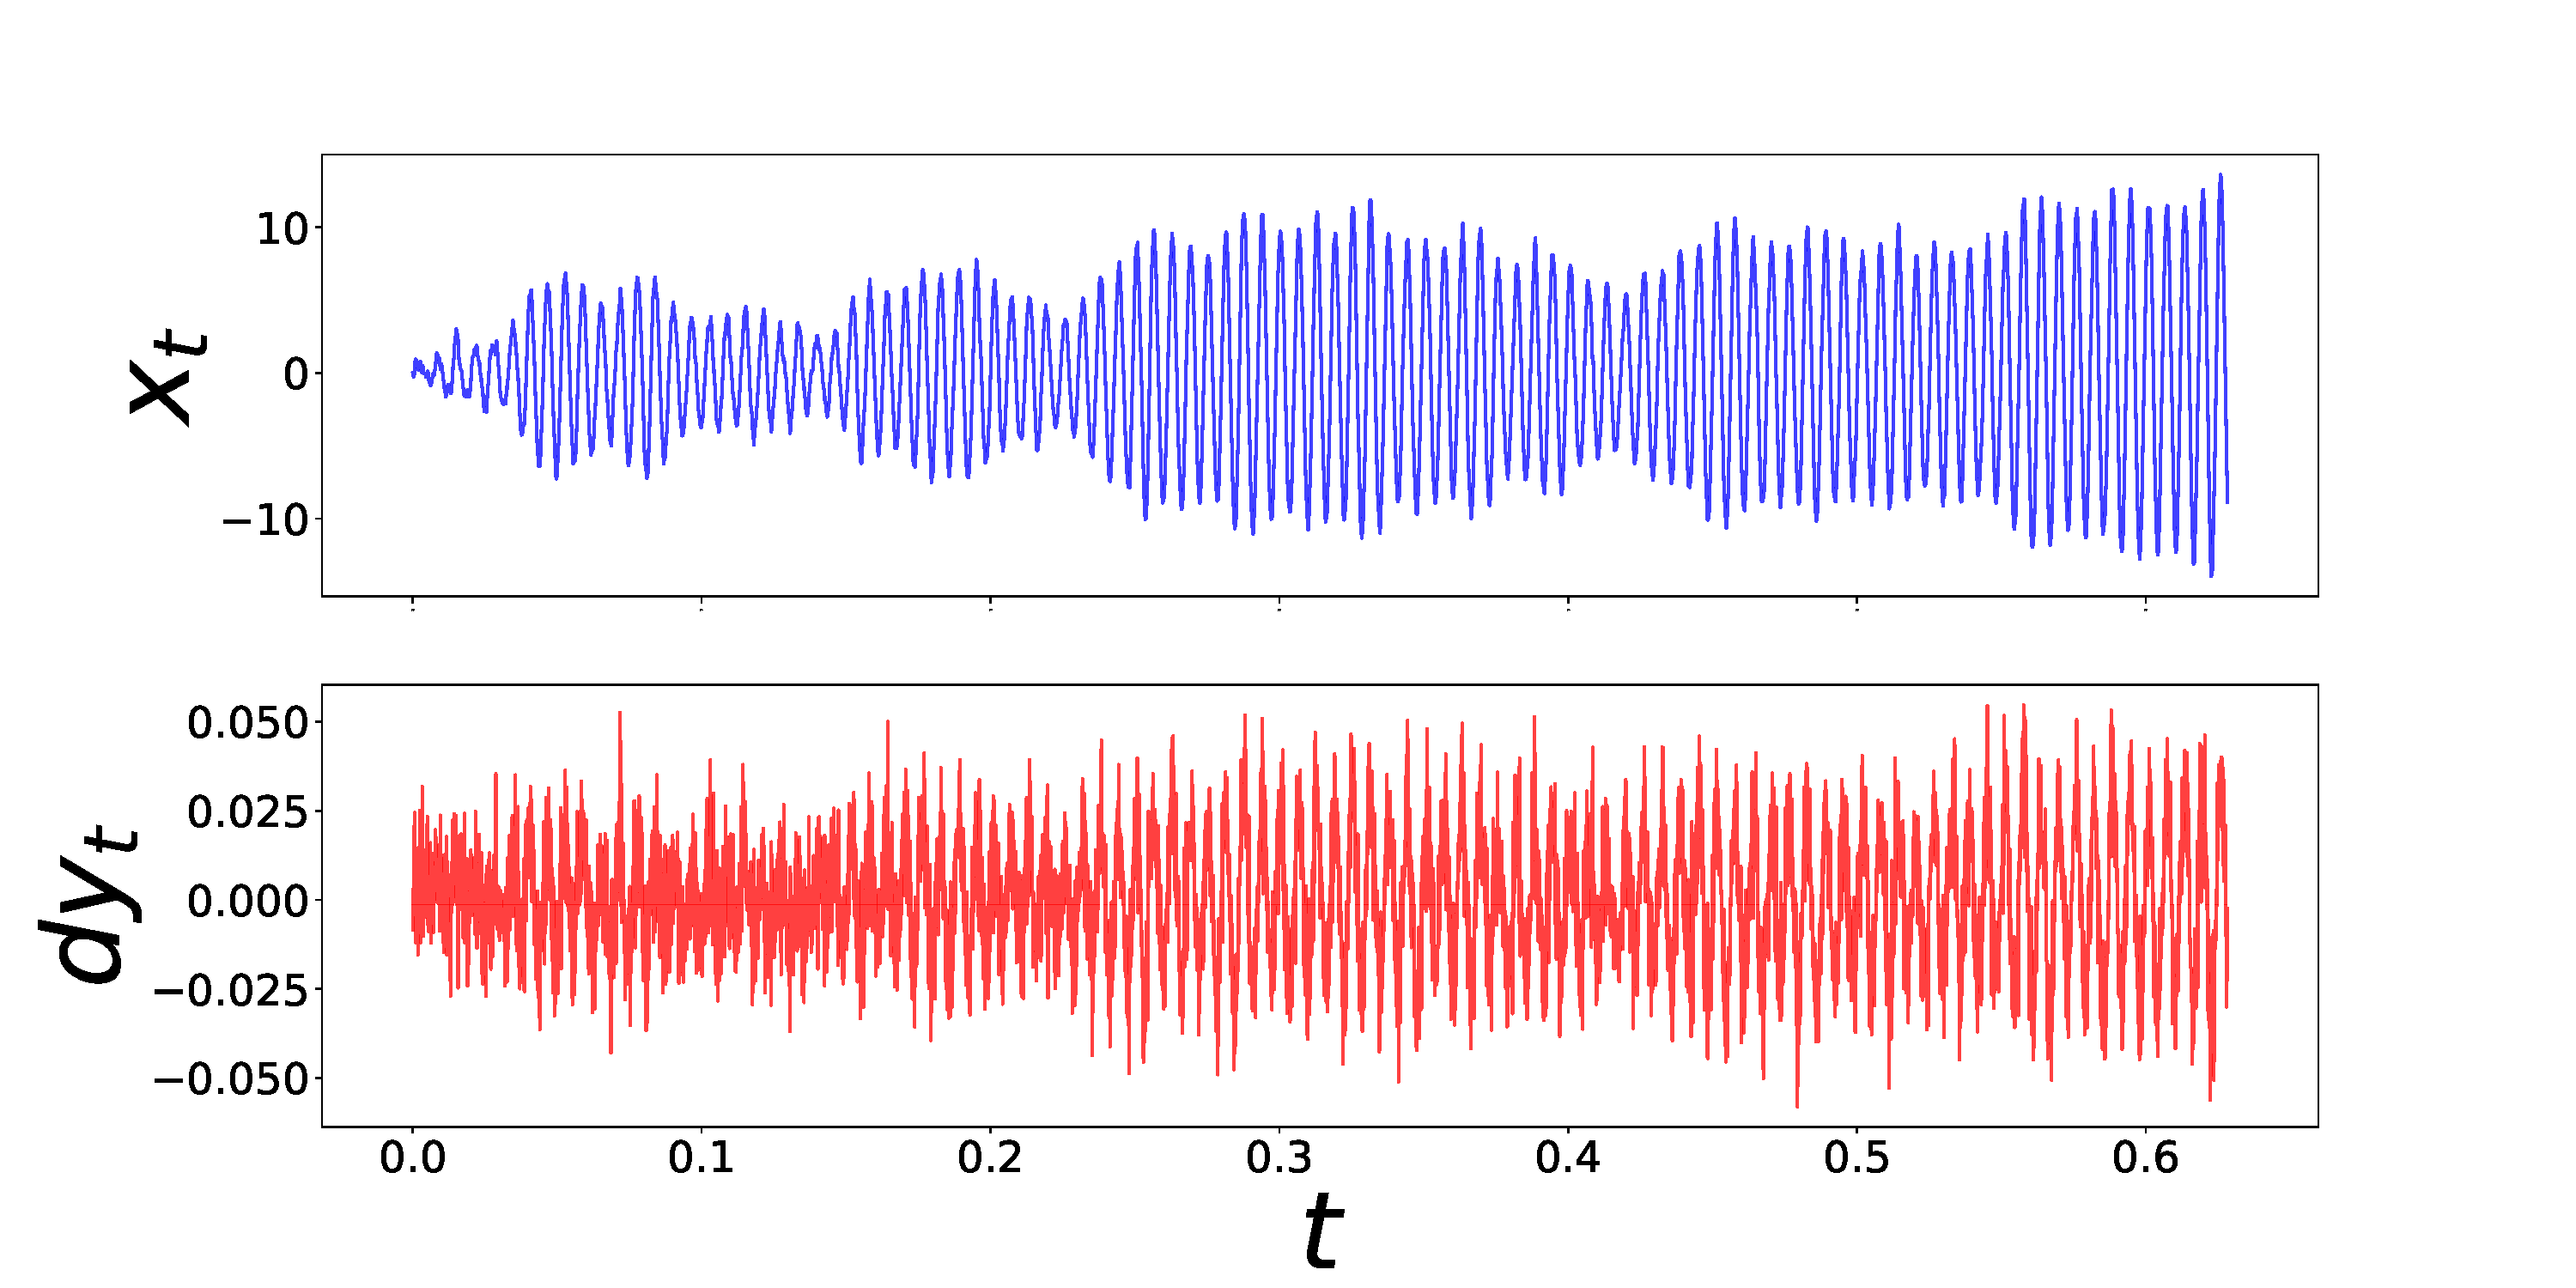
\includegraphics[width=1.\textwidth]{Figures/CMON/estimation/evolution.pdf}
    \caption{We show a realization of a quantum trajectory (top) along with the measurement record (bottom), for the process described by Eq.~\ref{eq:cmon_LINEALSYSTEM}}
    \label{fig:evol}
\end{figure}


Let us discuss further the structure of Eqs.~\ref{eq:cmon_LINEALSYSTEM} and Eq.\ref{eq:cmon_rica2}. Firstly, we note that the innovations $\dwt$ do only appear in the evolution for the first moment $\rbar_t$. In fact, the evolution for the covariance matrix given in Eq.~\ref{eq:cmon_rica2} is deterministic, and known as the continuous Ricatti equation; moreover we note that the final term causes a reduction in the uncertainty about the system state and is related to the measurement via $\chi(\cov)$. Furthermore, it can be shown that the Ricatti equation admits a stationary solution if the eigenvalues of $A$ have a non-positive real-part part, what is known as the Hurwitz condition\footnote{Intuitively, the imaginary part will contribute to the oscillatory behaviour, whereas the real part will either damp (positive) or magnify (negative) the signal, since the solutions are of the form $\expect{\rbar(t)} = e^{At}\rbar(0)$}, then the covariance will eventually converge to its stationary value
(\textit{i.e.} $d\cov_t = 0$), also known as stabilizing solution~\cite{Wiseman2005optimal}.

Secondly, we note that Eq.~\ref{eq:cmon_LINEALSYSTEM} is shown in two forms: either with the measurement outcome $\dyt$ or with the innovation $\dwt$. While the latter provides a clear interpretation of the evolution in the Ito form, being $A$ and $\chi(\cov_t)$ the drift and difussion terms, the innovations are not experimentally accesible. Rather, we do only have access to the measurement outcomes $\dyt$ in order to update our knowledge of the quantum-state, and thus the evolution should be understood from this perspective. In turn, this makes explicit the \textit{back-action} phenomena: gathering information about the system unavoidable affects its evolution. In this regard, the system can be understood as a Hidden markov model, where the measurement outcome $\dyt$ conditions the value of the hidden state $\bar{r}_{t+dt}$; such hidden state (as well as the covariance) is unavailable to us, but can be \textit{tracked}
by means of Eqs.~\ref{eq:cmon_LINEALSYSTEM} and \ref{eq:cmon_rica2}.

While the bayesian structure of quantum theory via the Born rule and the post-measurement states result in the aforementioned set of stochastic lineal equations for the Gaussian model under consideration, there is a classical counterpart. This analogy with the Kalman filter was firstly highlighted in Ref.~\cite{doherty1999feedback}, and a similar structure is obtained for the equations that update the first two moments of a Hidden Markov (Gaussian) system. In this regard, while the initial states of the system might be unknown, the equations steer an estimate of the first two moments in a contractive way, and via the measurement result $\dyt$, towards their (hidden) \textit{true} value. This holds, as long as the right dynamics is used in order to update such moments. On the contrary, if a wrong dynamics was used, a discrepancy between the measurement result (which takes the estimate towards the \textit{true} hidden state) and the update via the \textit{wrong} model will arise. This is captured by the log-likelihood distribution, \textit{i.e.} the probability of observing such measurement results under the corresponding model, and its evolution reduces in the Gaussian to
\eq{lambdaGauss}{d\lambda_t = -\frac{1}{2} ||C \rbar_t||^2 dt + C \rbar_t \cdot \dyt,}
where $\rbar_t$ is the solution of Eq.~\ref{eq:cmon_LINEALSYSTEM} at time $t$, and its dependence on $\Yt$ is implicit.

Whether we are using the right dynamics in order to update the hidden state value or not, is the matter hypothesis testing. As discussed in Sec.~\ref{ssec:1_hypo_testing}, the discrepancy between the two hypothesis is captured via the log-likelihood ratio, which for the Gaussian system under consideration obeys the dynamical equation
\begin{align}\label{eq:linealLog}
d\ell(\mathcal{Y}_{t|k}) = \frac{(-1)^{k+1}}{2}||C \Delta\rbar_t  ||^2 dt + C \Delta\rbar_t \cdot \dwt
\end{align}
where $\DeltaXt = \rbar_{1}(\mathcal{Y}_{t|k},t)-\rbar_{0}(\mathcal{Y}_{t|k},t)$ is the vector difference between the first moment of the Gaussian state generated through the null and alternative hypothesis dynamics. Here, each of the moments associated to the corresponding hypothesis is obtained by (numerically) solving the set of stochastic lineal equations Eqs.~\ref{eq:cmon_LINEALSYSTEM} and Eq.~\ref{eq:cmon_rica2} using the respective corresponding value for the coefficient matrices.

We will study two different scenarios: damping and frequency discrimination. The former will be analyzed in detailed, as some analytical results can be derived. Since our goal is to introduce sequential strategies for hypothesis testing in continuously-monitored systems, the very same approach can be used to test different models, and thus using it on frequency discrimination problems serves as an extra numerical \textit{check}.

\subsubsection{Damping discrimination}
We will now consider the scenario where a model is captured by a specific value of the mechanical mode's damping rate $\gamma$. The null hypothesis is given by $\gamma = \gamma_0$ and the alternative hypothesis by $\gamma = \gamma_1$, with all the remaining coefficients (namely $\eta$, $n$ and $\kappa$) being shared by the two models. We will study the case in which the system is analyzed in a frame that rotates with the mechanical-mode's frequency, and thus the coefficient matrices $A$ and $C$ are given by Eq.~\ref{eq:homodyneROT}. In this case, the quadratures become uncoupled (since $A$ is now diagonal), and both quadratures are affected by the same dynamics. Thus, we can expect the stationary value of the covariance matrix to be diagonal. Moreover, in this case the Ricatti equation admits a closed-form solution for its stationary value under hypothesis $k$, namely $\cov_k = \sigma_k \mathbb{I}_2$ with
\begin{align}\label{eq:stat_cov_damping}
\sigma_k &= \frac{\gamma_k}{8\eta \kappa}\Big(\sqrt{1 + \frac{16 \eta \kappa \sigma_{k,uc}}{\gamma_k}} -1 \Big) \\
\sigma_{k,uc} &= n + \frac{1}{2} + \frac{\kappa}{\gamma_k},
\end{align}
where $\sigma_{k,uc}$ is the solution for the unconditional evolution of the covariance in Eq.~\eqref{eq:cmon_unco}. Because Hurwitz conditions are satisfied for the system under consideration (and in order to save some computing resources), our simulations already start from the stationary state. In case that a closed-expression for such stable solution is not available, as it happens when studying cavity dynamics with non-trivial Hamiltonians~\cite{Fallani2022Learning}, or without moving to a rotating-frame, we rely on numerical methods to solve the Ricatti equation and provided by Refs.~\cite{scipy,schurCARE}.

\begin{figure}[t!]
    \centering
    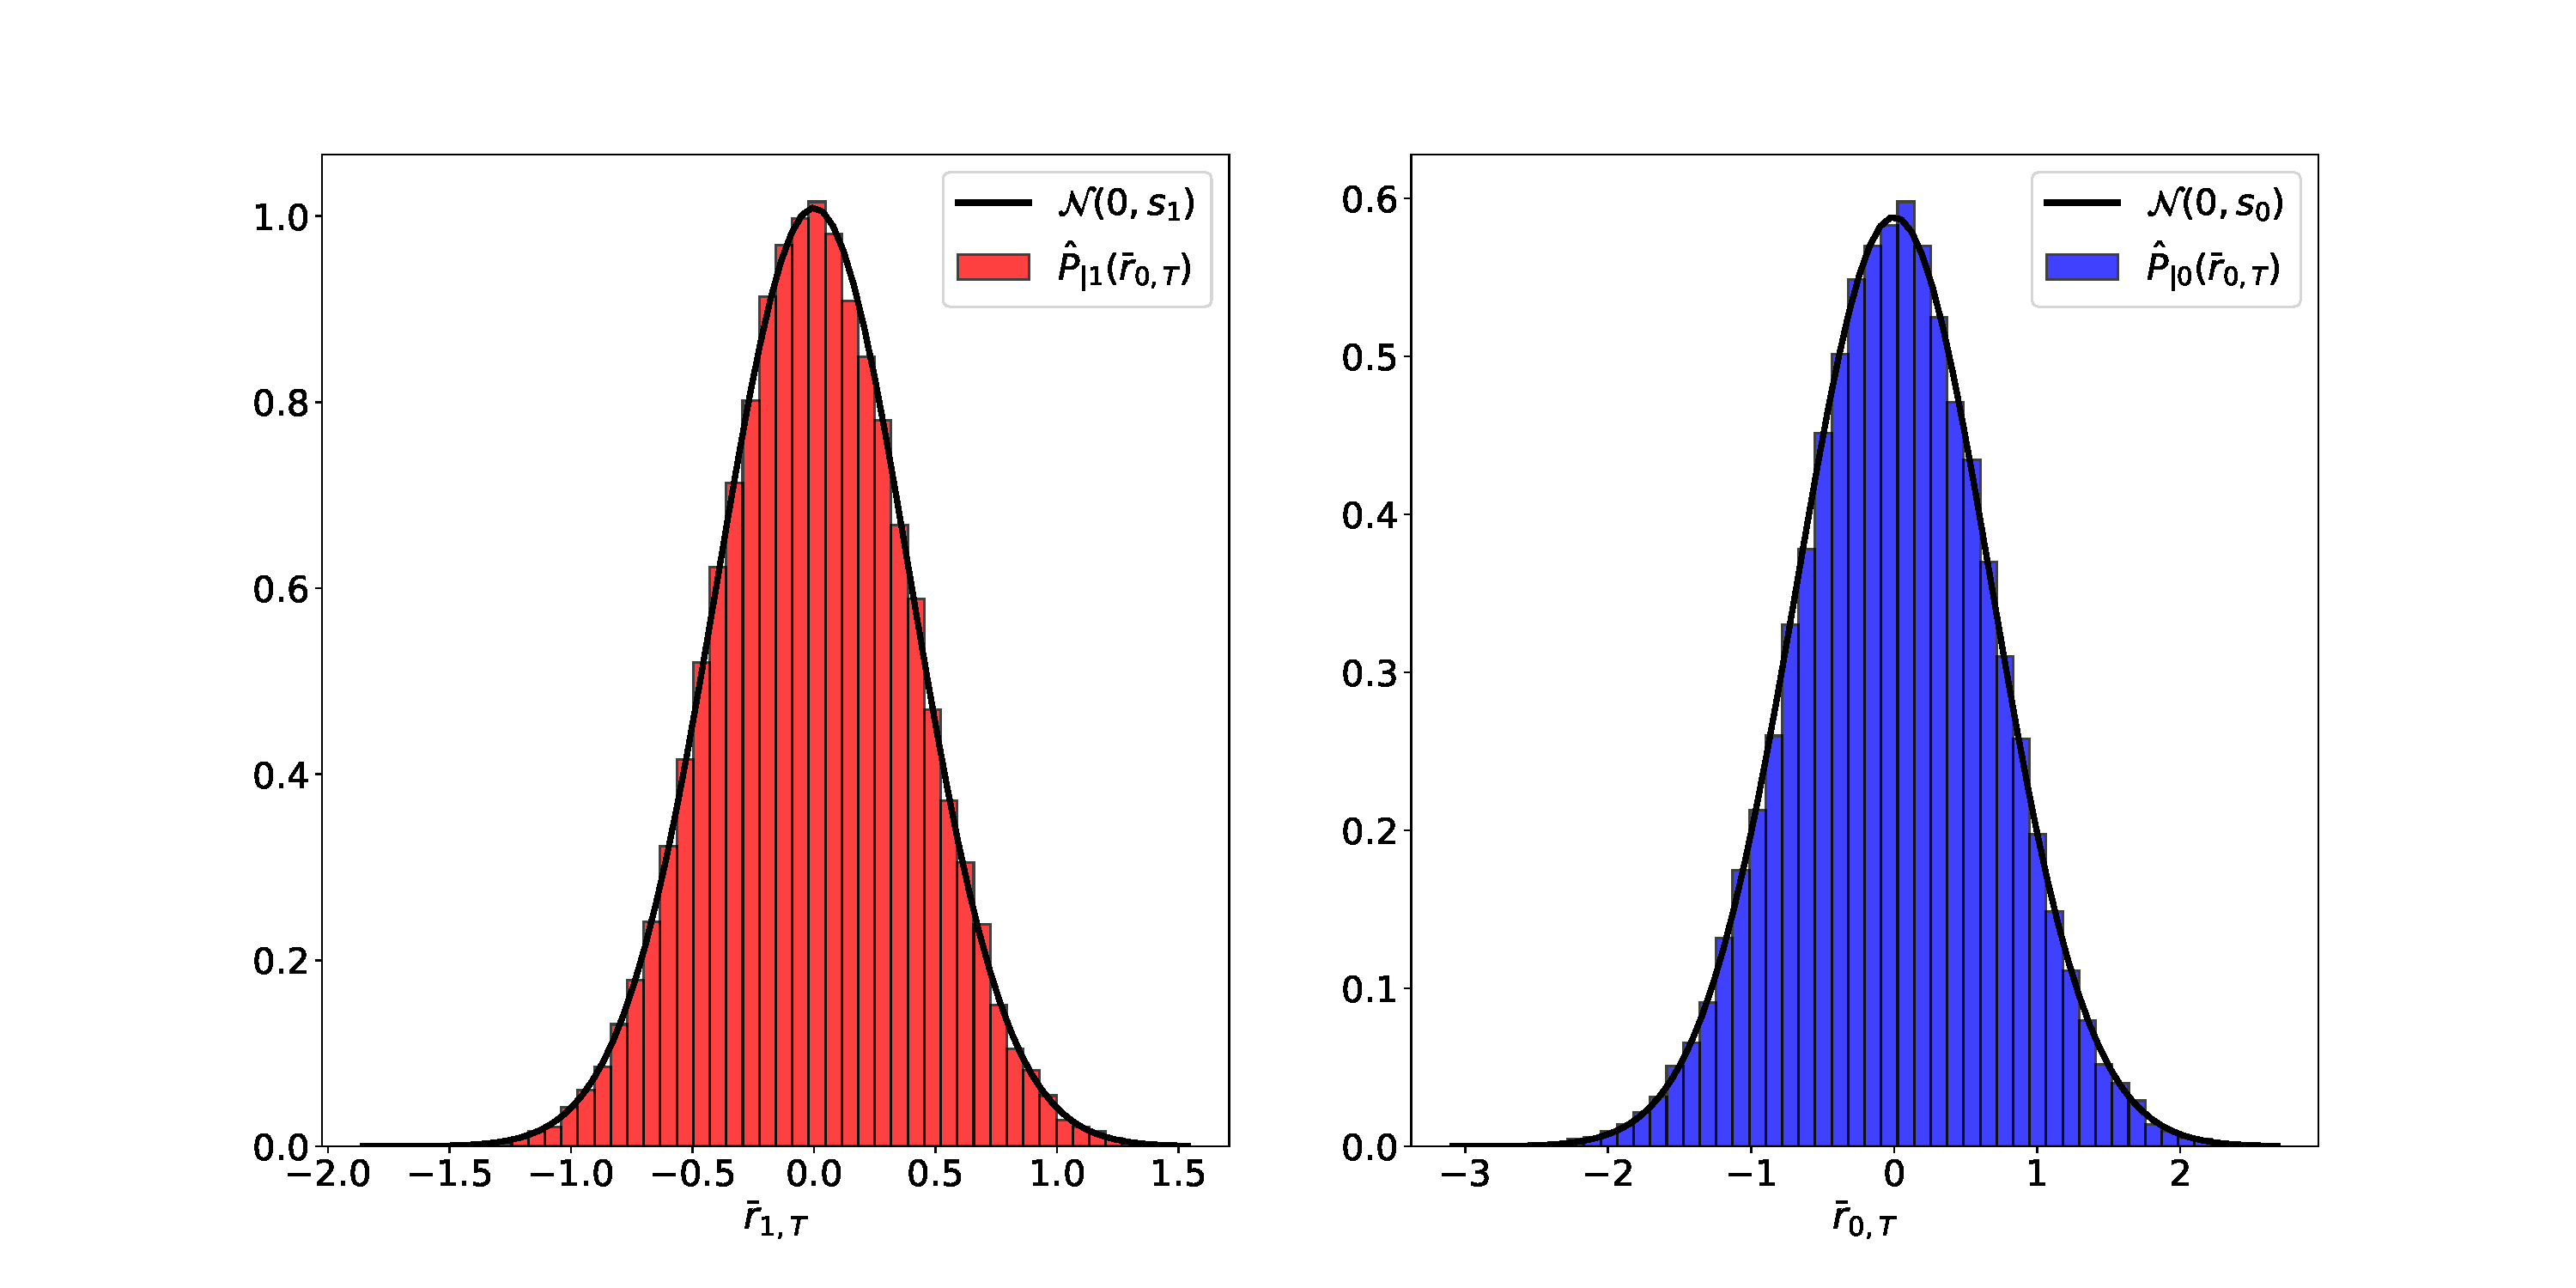
\includegraphics[width=1.\textwidth]{Figures/CMON/damp-discri/distributions_hidden.pdf}
    \caption{The distributions for the hidden states are shown, simulated under the alternative ($\gamma = 429 $ Hz) and null hypothesis ($\gamma = 100$ Hz) respectively. The histograms are obtained by simulating $2 \cdot10^{4}$ quantum trajectories, and the time for which the distributions are displayed is $T=4s$.}
    \label{fig:cmon_distributions_hidden}
\end{figure}

Let us now study the evolution of the hidden-state $\rbar_{k,t}\equiv\rbar_k(t)$. Assuming hypothesis $k$ is the true one, the solution of $\rbar_k(t)$ reads
\eq{rkstoch}{\rbar_k(t) = e^{A_kt}\rbar_k(0) + \chi(\cov_k)\int_{0}^t e^{A_k(t-\tau)} \dwtau,}
where we have expressed Eq.~\ref{eq:cmon_LINEALSYSTEM} as an integral stochastic equation. From our discussion of Ito calculus in Sec.~\ref{ssec:ito}, we can expect that the average value\footnote{Note that this average is over several realizations of the stochastic process, \textit{i.e.} over different quantum trajectories, and as such is a \textit{classical} one.} $\expect{\rbar_{k,t}}\underset{t\rightarrow0}{\longrightarrow}0$ for any initial condition $\rbar(0) = (q_0, p_0)$.
Moreover, we can readily compute the variance in the long-time regime, \textit{i.e.} $\mathbb{E}[\rbar_k^2]$, which reads
\begin{align}\label{eq:vkst}
\mathbb{E}[\rbar_k^2] = \frac{8 \eta \kappa \sigma_k^2}{\gamma_k} := s^2_k
\end{align}
Thus, the first moment of the hidden state $\rho_k$, evolved under hypothesis $k$, is Gaussian distributed with zero mean and a variance $s^2_k$ given by Eq.~\ref{eq:vkst}. This is illustrated in Fig.~\ref{fig:cmon_distributions_hidden}, where the probability distribution of the hidden state is shown at a large time, and compared with numerical simulation of the (Gaussian) quantum trajectories. Here, and in most of the plots shown in this section the simulations are based on the following choice of parameters:  $\gamma_{0}=100$ Hz for $H_{0}$ and $\gamma_{1}=429$ Hz for $H_{1}$, while the rest of the parameters are taken to be same for both hypotheses
 $n:=n_{0}=n_{1}=1, \eta=\eta_0=\eta_{1}=1, \kappa=\kappa_{0}=\kappa_{1}=9$ Hz.

\subsection{The log-likelihood ratio}
As discussed above, chances exists that the \textit{state of knowledge} of our quantum system is being updated with the \textit{wrong} model. For simplicity, let us assume that hypothesis $1$ generates the data, and thus $\dyt = C\big(\rbar_{1,t} + C^{-1} \dwt\big)$. While both hypothesis are updated using $\dyt$, as per Eq.~\ref{eq:cmon_LINEALSYSTEM}, the crucial matter is to reduce the possibilities of telling that null hypothesis $k=0$ is the true one (we will later consider the symmetric error). Recalling that the evolution for $\rbar_{0}(t)$ reads
\begin{align}
d\rbar_{0,t} = \big[A_0 - \chi(\cov_0)\big]\rbar_{0,t} dt + \chi(\cov_0) C \rbar_{1,t} dt + \chi(\cov_0) \dwt,
\end{align}
where we have expanded the $\dyt$ term in Eq.~\ref{eq:cmon_LINEALSYSTEM}, then the integral expression reads\footnote{Note that we have dropped the deterministic term proportional to $e^{(A-\chi(\cov_0)t)}\rbar_0(0)$ since we are concerned with the long-time regime.}
\begin{align}\label{eq:expec_state_true}
\rbar_{0}(t) = \chi(\cov_0)C\int_{-\infty}^t e^{\Big[A_0 - \chi(\cov_0 C)\Big](t-\tau)} \rbar_1(\tau) d\textbf{W}_\tau +
\chi(\cov_0)\int_{0}^t e^{\Big[A_0 - \chi(\cov_0 C)\Big](t-\tau)} \dwtau.
\end{align}
Recalling that $\rbar_1(t)$ is given by Eq.~\ref{eq:rkstoch} for $k=1$, and using the stochastic integration rule outlined in Sec.~\ref{ssec:ito}, we can readily compute the following expected values in the long-time regime ($t\to\infty$)\footnote{Exact expressions for all times can be also computed, but we refrain from giving them explicitly here.}:
\begin{align}\label{eq:expect_states_alt}
\mathbb{E}_1[\rbar^2_{0}] &= \frac{8 \sigma_0^2 \eta \kappa}{\gamma_0 + 8 \sigma_0 \eta \kappa}\Big(1 + \frac{16 \sigma_1 \eta \kappa}{\gamma_0 + \gamma_1 + 8 \sigma_0 \eta \kappa} + \frac{(8 \sigma_1 \eta \kappa)^2}{\gamma_1(\gamma_0 + \gamma_1 + 8\sigma_0 \eta \kappa)}\Big), \\
\mathbb{E}_1[\rbar_0\rbar_1]&= \frac{32 \sigma_0 \sigma_1 \eta \kappa }{\gamma_0 + \gamma_1 + 8\sigma_0 \eta \kappa}\Big(1+\frac{4\sigma_1\eta \kappa}{\gamma_1}\Big).
\end{align}
We note that in the case that hypothesis $0$ was the underlying one (\textit{i.e.} generating $\dyt$) then the above expressions are identical, but swapping the values of $\gamma_1$ and $\gamma_0$.

\begin{figure}[t!]
    \centering
    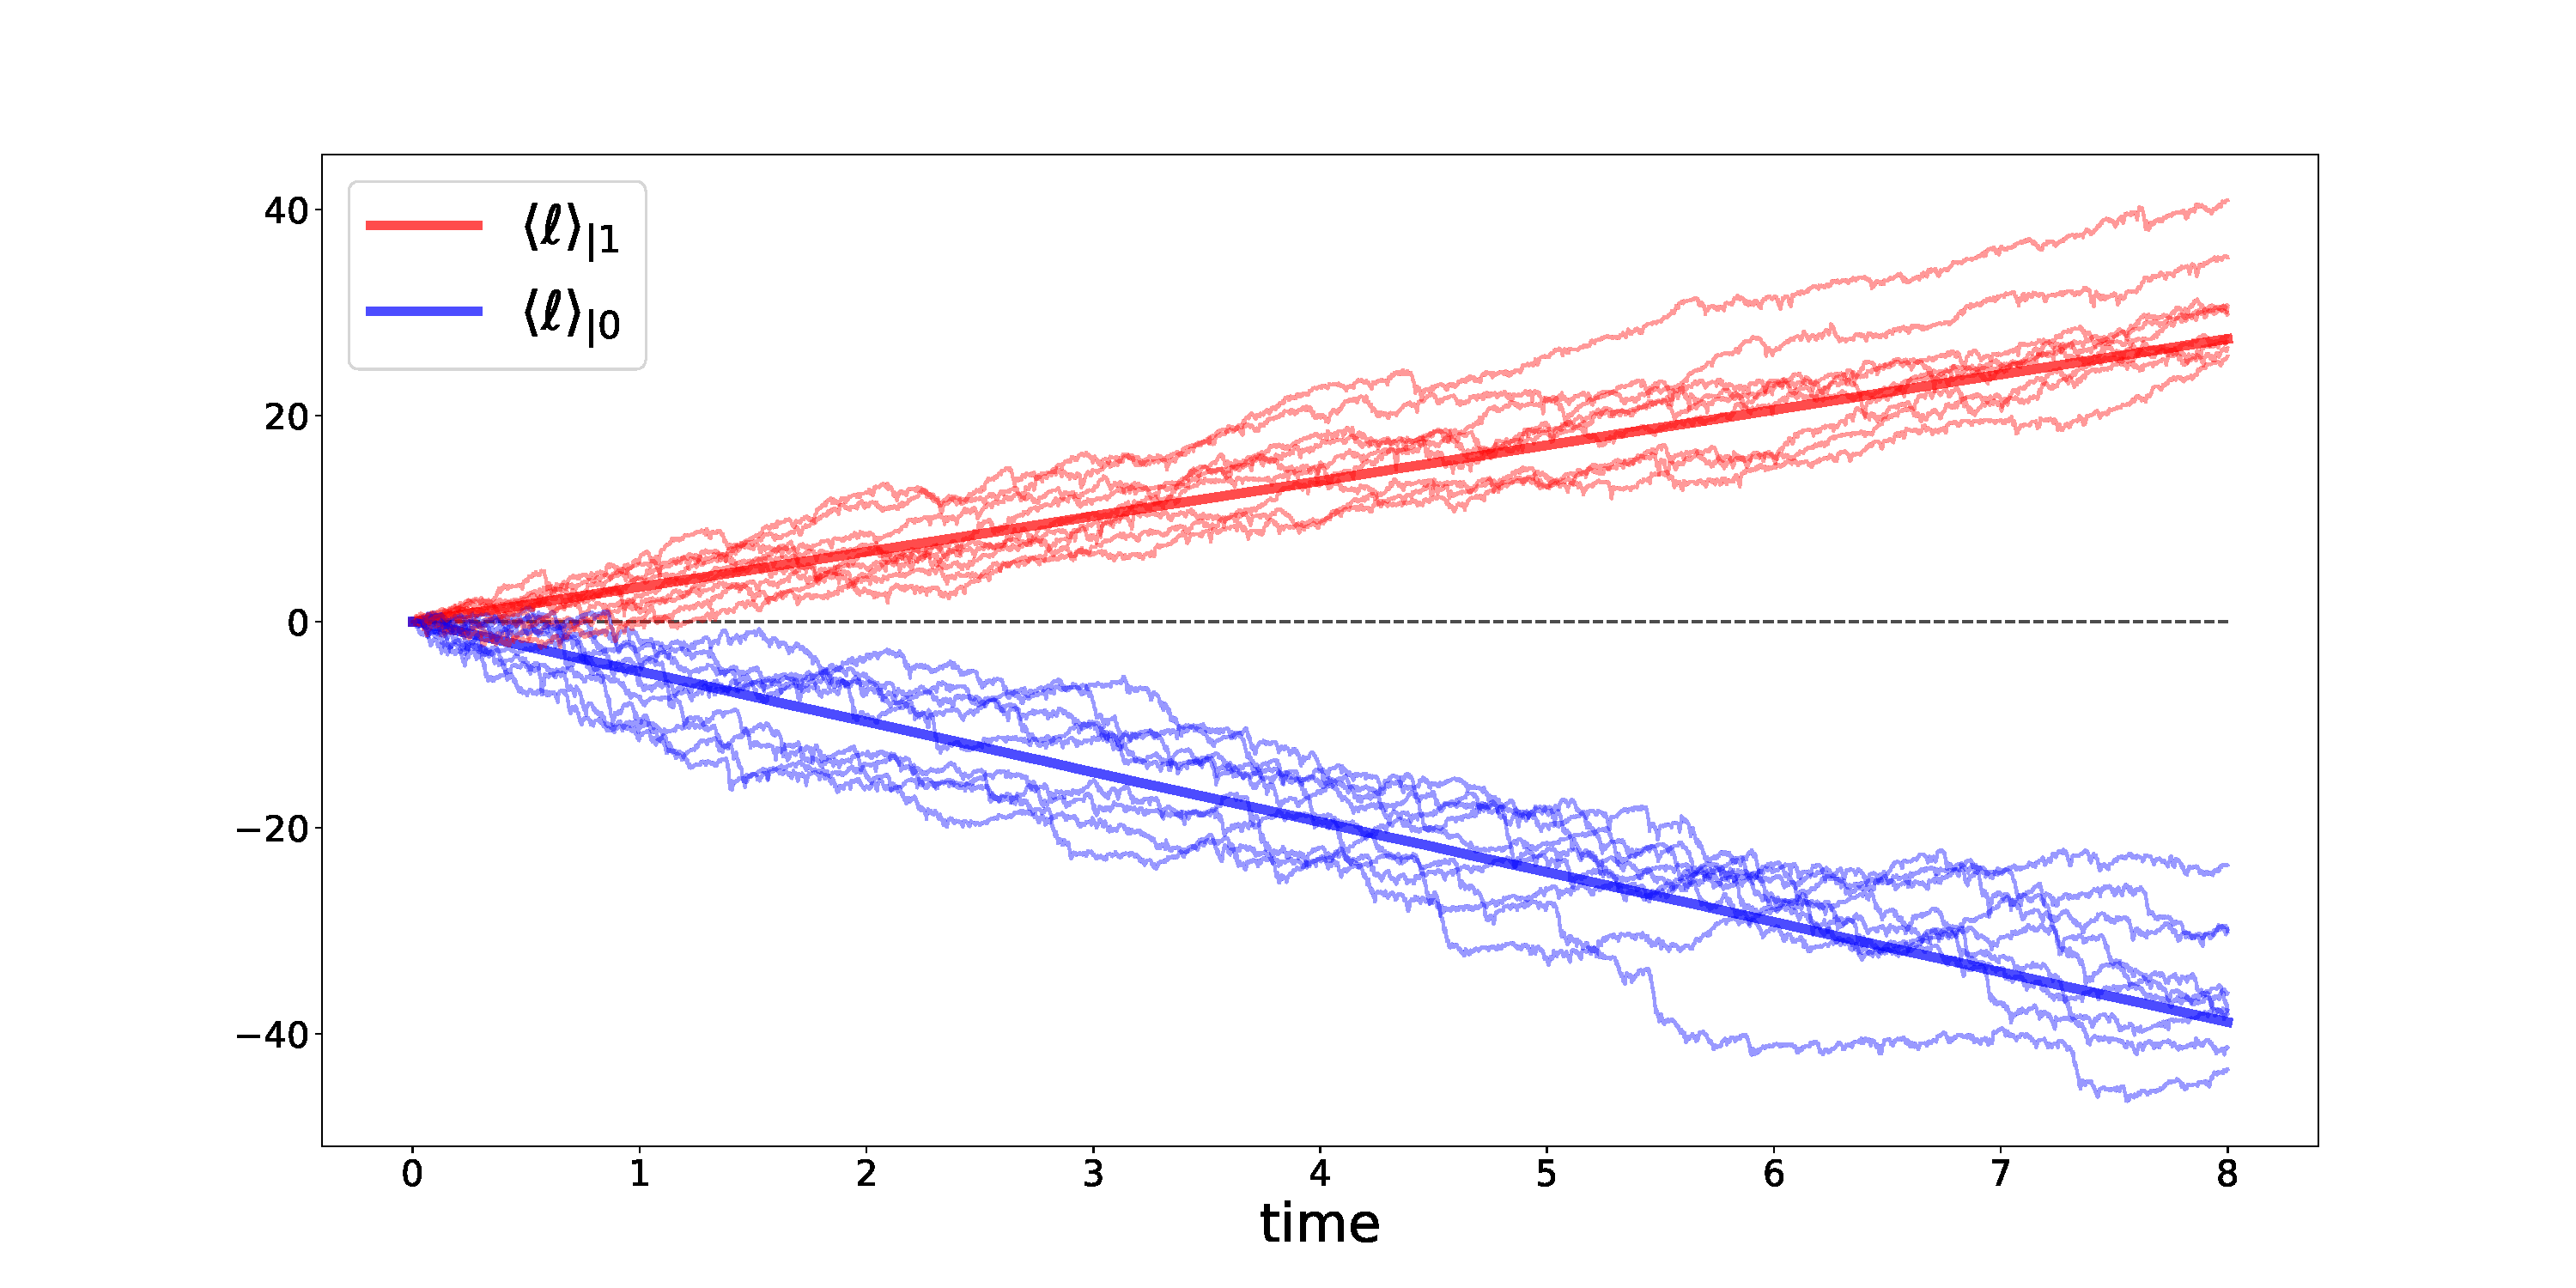
\includegraphics[width=1.\textwidth]{Figures/CMON/damp-discri/temp/avg_ell_time.pdf}
    \caption{We show the stochastic evolution of the log-likelihood ratio under both models, together with its empirical average computed over $2 \cdot 10^{4}$ trajectories, for the damping discrimination problem considered in this Section.}
    \label{fig:liks_drfit}
\end{figure}

Combining these expressions with Eq.~\ref{eq:linealLog}, we can readily find the expected value of $\ell$ under hypothesis $k$. To see this, we take the expectation value, to get
\begin{align}\label{eq:dlav}
\mathbb{E}_k[d\ell_{t}] = \frac{(-1)^{k+1}}{2}\mathbb{E}\Big[||C \Delta\mathbf{r}_t  ||^2 \Big] dt = (-1)^{(k+1)} \mu_k dt
\end{align}
where in the last equality we have used the stationary value (long time regime) of the effective drift coefficient. Inserting the previous results we get an analytical expression for the value of $\mu_1$
at $t\to\infty$,
\begin{align}\label{eq:mukANAL}
\mu_1 = \frac{c^2(\gamma^2_1\chi^2_0 + 2c\gamma_0(\chi_0 - \chi_1)^2 + \gamma_0^2\chi_1^2 + \gamma_0\gamma_1(\chi_0^2 - 4\chi_0\chi_1 + \chi_1^2)}{\gamma_0(\gamma_1 + 2 c \chi_1)(\gamma_0 + \gamma_1 + 2 c \chi_1)},
\end{align}
where $\chi_k = c \sigma_k$, with $\sigma_k$ given by Eq.~\ref{eq:stat_cov_damping} and $c = \sqrt{4\eta\kappa}$. The expression for $\mu_0$ is obtained by swapping $\gamma_0$ and $\gamma_1$. It is important to note that the two drifts do always differ. Similarly, we can compute the variance of $\ell$, which we anticipate scales linearly with time, and its full analytical expression is, at least, scaring. We will discuss an alternative approach to compute these two moments in (for general system parameters) later in the Sec.~\ref{ssec:oucoupled}, where we consider the  evolution of an extended system, comprising the dynamics of both models, $\rbar_{0}$
and $\rbar_{1}$, effectively coupled by the common measurement record, as an Orstein-Uhlenbeck process.

From \eqref{eq:dlav} and \eqref{eq:mukANAL} we readily find that the expected value of the log-likelihood function at long times is given by
\begin{align}\label{eq:dint}
\mathbb{E}_k[\ell_{t}]  =\int_{0}^{t}\mathbb{E}_k[d\ell_{t}]= (-1)^{k+1} \mu_k t +\mathcal{O}(1)
\end{align}
where $\mathcal{O}(1)$ accounts for the finite contribution to the integral of the time it takes for $\mu_{1}(t)$ to reach its stationary value.

We have conducted numerical simulations of a possible measurement records $\Yt$ obtained for both
models under consideration and  computed  the the log-likelihood statistic  $\ell_{t}(\Yt)$ according to the above sequential presecription.
This is depicted in Fig.~\ref{fig:liks_drfit}, where the average value of $\ell_{t}$ is shown for both models, accompanied by some realizations of the process. As expected, we observe a positive drift when the alternative hypothesis is the underlying one, and a negative drift in the opposite case. Moreover, the mean and variance of the log-likelihood (averaged out over different quantum trajectories) are compared to their theoretical values in Fig.~\ref{fig:cmon_momentos}.

\begin{figure}[t!]
    \centering
    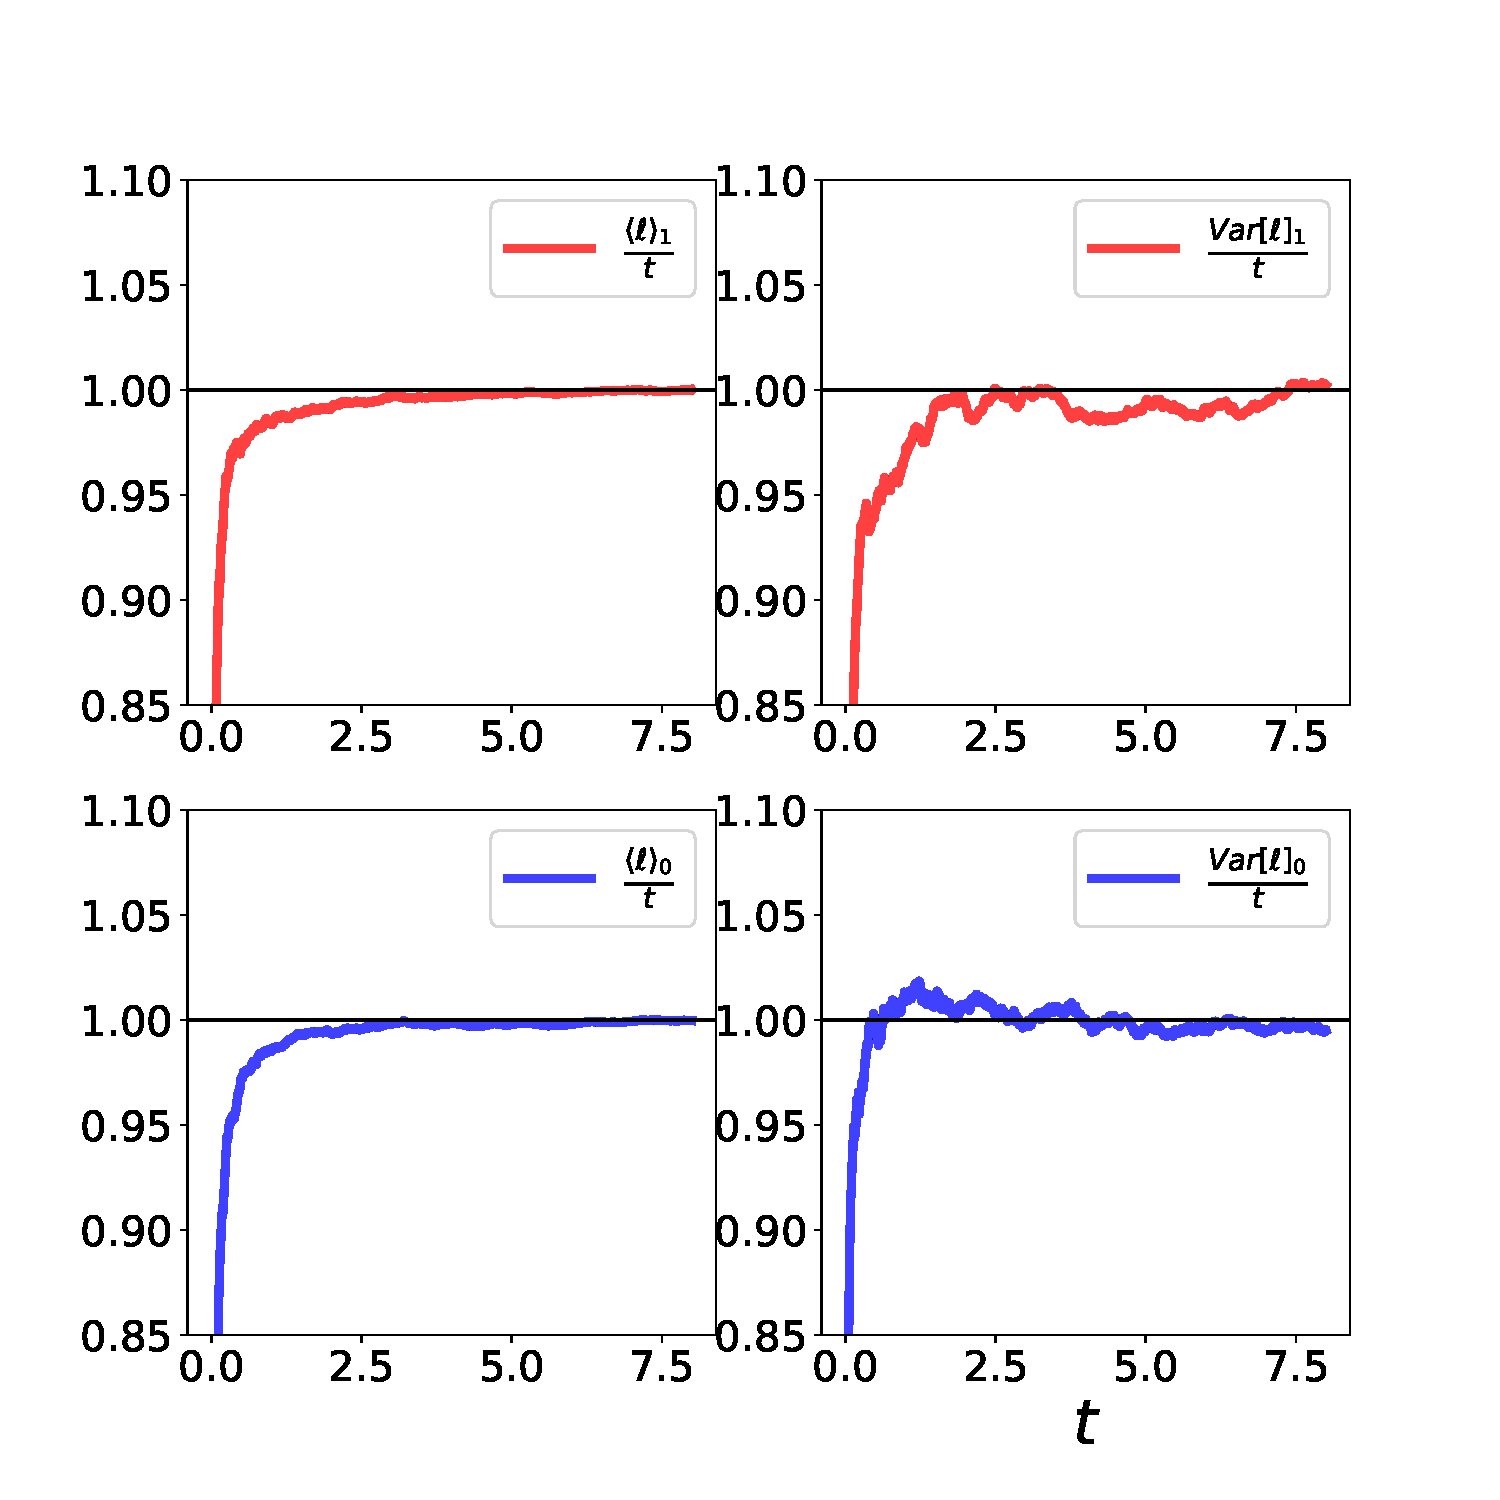
\includegraphics[width=1.\textwidth]{Figures/CMON/moments.pdf}
    \caption{We compare the first two moments estimated over $2 \cdot 10^{4}$ trajectories with their predicted theoretical value, for both hypothesis, in the damping discrimination scenario under consideration.}
    \label{fig:cmon_momentos}
\end{figure}

Having validated the stochastic equation for the log-likelihood we can compute the average stopping time of a sequential test. Recall that the Sequential Probability Ratio Test (SPRT) stops as soon as one can guarantee a large probability of success (what we called strong error conditions):
\begin{align}\label{eq:serr2}
p(H_1|\Yt) &\geq 1-\epsilon_{0}, \\
p(H_0|\Yt) &\geq 1-\epsilon_{1}.
\end{align}

If none of these two conditions are satisfied, the test continues, \textit{i.e.} further samples are requested. Following the same reasoning than standard SPRT for the \textit{i.i.d.} case discussed in Sec.~\ref{ssec:sprt}, these conditions can be equivalently expressed in terms of the log-likelihood ratio $\ell$, by fixing an \textit{undecision region} $\Omega = [-a_{0},a_{1}]$.
For simplicity of the presentation we will treat the hypothesis on an equal footing, and set $\epsilon=\epsilon_0 = \epsilon_1$ and equal prior
$\pi_0 = \pi_1=1/2$ (the results are easily extended to more general settings), resulting in
\eq{decisionsASPRT}{a=a_0 = -a_1=\log{\tfrac{1-\epsilon}{\epsilon}}.}
The test stops as soon $\ell_{t}$ first hits a boundary of $\Omega$\footnote{Note that if the test did not stopped, then chances are that $\ell$ hit such boundaries also at later times for the same trajectory.} and guesses for $\hat H_{1}$ ($\hat H_{0}$) when it hits the upper (lower) boundary.

Recall that the values of type I and II errors for such sequential test can be computed from the consistency equation (\textit{i.e.} Eq.~\ref{eq:weakErrorsSPRT}),
\begin{align}\label{eq:cmon_sprt_weak}
\alpha &= p(\hat{H}_1|H_0) = e^{-a}(1-\beta)\\
\beta &= p(\hat{H}_0|H_1) = e^{-a} (1-\alpha),
\end{align}
leading to
$ \alpha  =\beta=\frac{1}{1+e^{a}}=\epsilon$, as it should since the error is guaranteed to be $\epsilon$
for each single trajectory (the inequalities in strong error conditions \eqref{eq:serr2} are saturated because
the likelihood is a continuous stochastic function).


Next note that the limit of large $a$ (long times),
\begin{align}\label{eq:cmonWlad}
\mathbb{E}_k[\ell_{\tau}] & =\mathbb{E}_k[\int_{0}^{\tau} d\ell_{t}]=
 \mathbb{E}_k[\int_{0}^{\infty} \mathcal{I}_{t<\tau} d\ell_{t}]=\int_{0}^{\infty} \mathbb{E}_k[\mathcal{I}_{t<\tau}]\mathbb{E}_k[d\ell_{t}]\\
 &= \mu_{k}\int_{0}^{\infty} \mathbb{E}_k[\mathcal{I}_{t<\tau}] dt+\mathcal{O}(1)
=\mu_{k} \mathbb{E}_k\left[\int_{0}^{\infty} \mathcal{I}_{t<\tau} dt\right]+\mathcal{O}(1)=\\
 %\mu_{k}\int_{0}^{\infty}P({t<\tau})dt+\mathcal{O}(1)\\
 &=\mu_{k} \mathbb{E}_k\left[\int_{0}^{\tau} dt\right]+\mathcal{O}(1)=\mu_{k}\mathbb{E}_k[\tau]+\mathcal{O}(1)
\end{align}
where we have defined the indicator function $\mathcal{I}_{C}=1$ if condition $C$ is fulfilled  and  $\mathcal{I}_{C}=0$ otherwise, we have used that $\mathcal{I}_{t<\tau}=\mathcal{I}_{\ell_{t}\notin \Omega}$ and $d\ell_{t}$ are independent stochastic variables, and  that $\mathbb{E}_k[d\ell_{t}]$ becomes constant $\mu_{k}$ in a finite decay time.

Because of the continuity of $\ell_{t}$, there is is no overshooting, and the stopping time $\ell_{\tau}$ has the value at the boundary $\ell_{\tau}=\pm a$. Therefore, following the same arguments than in the \textit{i.i.d.} case in Eq.~\eqref{eq:mean_ell_binarySPRT}, we get
\begin{align}
\expect{\ell_{\tau}}_{1} &= a (1-\beta) - a \beta=a=\tfrac{1-\epsilon}{\epsilon}\\
\expect{\ell_{\tau}}_{0} &= -a (1-\alpha)+ a \alpha=a=\log{\tfrac{1-\epsilon}{\epsilon}}
\end{align}
Putting the pieces together, we finally arrive to a closed expression for the mean stopping time
\begin{align}\label{eq:waldcmon}
\mathbb{E}_k[{\ell_\tau}] &= (-1)^{k+1}\mu_k \mathbb{E}_k[\tau]+\mathcal{O}(1)=(-1)^{k+1} a+\mathcal{O}(1) \\
& \downarrow  \nonumber\\
\mathbb{E}_k[\tau]&= \frac{a}{\mu_{k}}+\mathcal{O}(1)=\frac{\log{\tfrac{1-\epsilon}{\epsilon}}}{\mu_{k}}+\mathcal{O}(1) \label{eq:waldcmon3}
\end{align}
where, as mentioned above, the $\mathcal{O}(1)$ term is due to the stabilization time of $\mu_{k}(t)$ (see Fig. \ref{fig:cmon_momentos}). Moreover, in the asymptotic limit of small errors
we get
\begin{align}\label{eq:waldcmon2}
\mathbb{E}_k[\tau]=-\frac{\log{{\epsilon}}}{\mu_{k}}+\mathcal{O}(1).
\end{align}
\begin{figure}[t!]
    \centering
    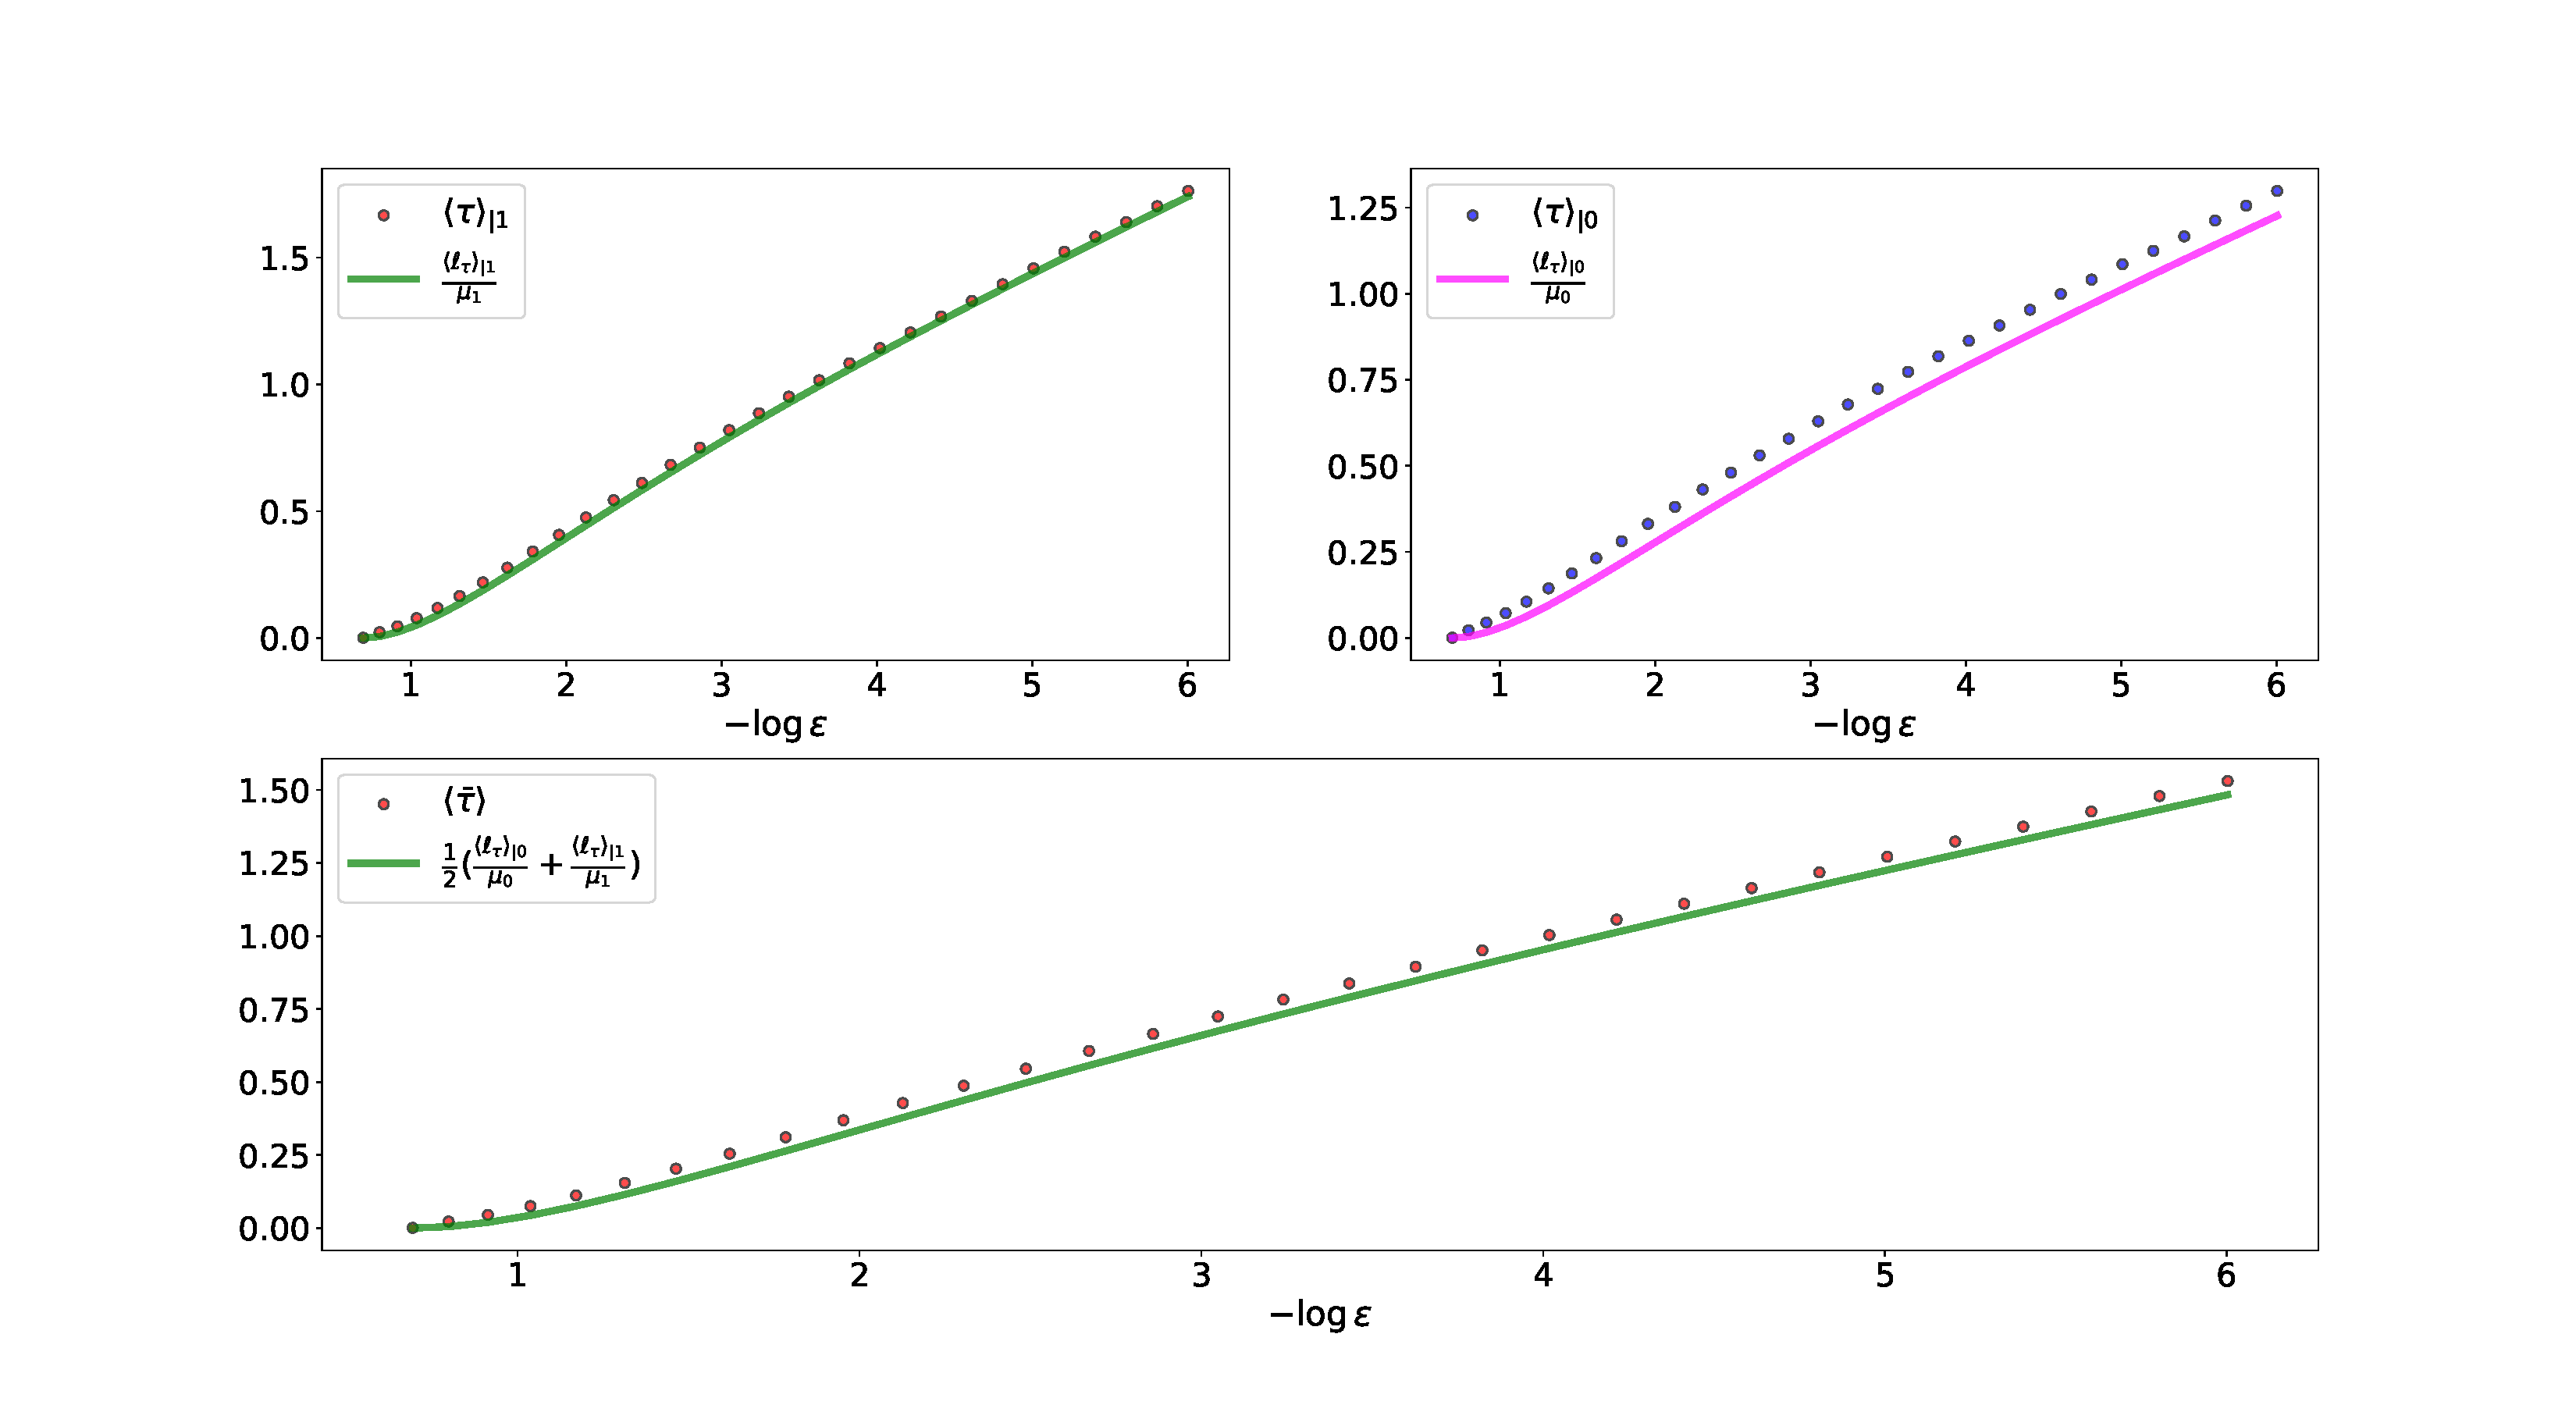
\includegraphics[width=1.\textwidth]{Figures/CMON/damp-discri/temp/wald_gamma429.pdf}
    \caption{We compare the average stopping time (under each hypothesis and also its mean value) with our analytical curve given in Eq.~\ref{eq:waldcmon}.}
    \label{fig:cmonwald}
\end{figure}

In Fig.\ref{fig:cmonwald} we show the mean stopping time as a function of the error threshold
corresponding to our numerical ``experiments'', for each of the hypothesis, and also the average
for both equiprobable hypotheses. We see a perfect consistency  w.r.t. our analytical predictions, namely the asymptotic linear scaling of stopping time $\expect{\tau}=\mu_{k}^{-1} \log\epsilon$. This results agree very well with the \textit{i.i.d.} case, $\expect{\tau}_{k}=D(P_{k}||P_{k+1})^{-1} \log\epsilon$, were now we replace the relative entropy $\expect{\ell_{i}}_{k}=D(P_{k+1}||P_{k})$ by its regularized version $\lim_{t\to\infty}\expect{\ell_{t}}_{k}=\mu_{k}$.

Note that Eq.~\eqref{eq:waldcmon3} gives an accurate assessment of the time it takes to reach a decision (withing a guaranteed error bound), though however it only provides its average value. Thus, a real-life experiment could actually end before or after such average value. In order to characterize the size of the fluctuations we need to understand how $\ell_{t}$ is distributed (see Fig.\ref{fig:cmonwald}).

\begin{figure}[t!]
    \centering
    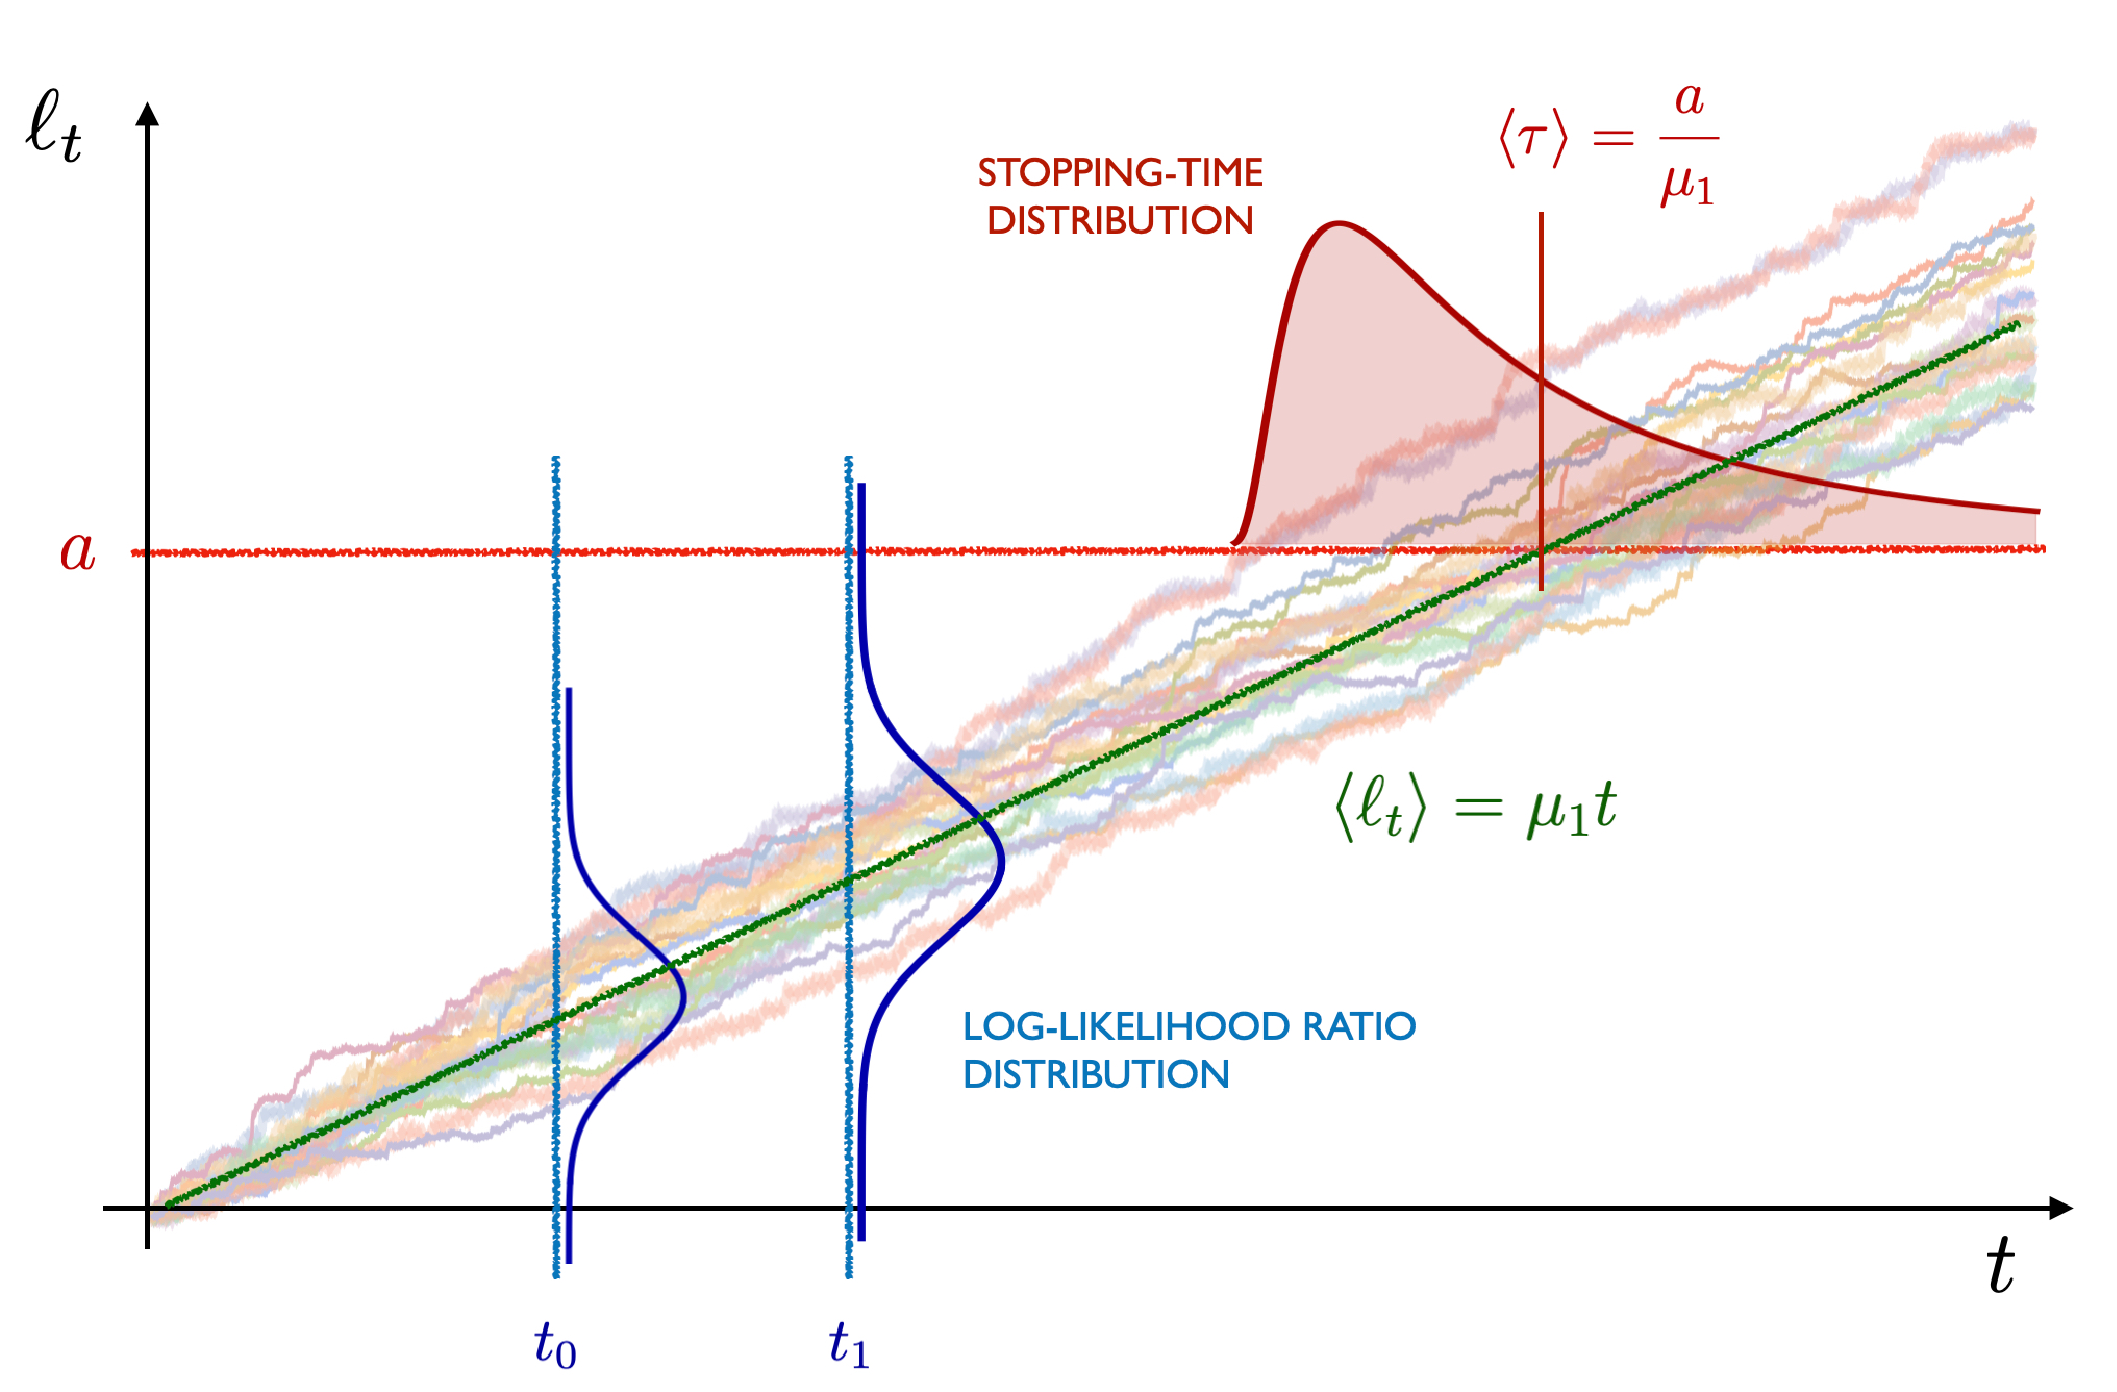
\includegraphics[width=1.\textwidth]{Figures/john_final_wald.pdf}
    \caption{We illustrate how the stopping time distribution arises from
    the random trajectories of $\ell_{t}$; here we show some realisations of the $\ell$ process, along with some time-slices at $t_0$ and $t_1$ shown in blue together with the  corresponding distributions $P(\ell_t)$. The horizontal line in red corresponds to the fixed threshold $\ell=a$, leading to an arrival time distribution $P(\tau)$. Such distribution appears as a consequence of a difference in the arrival times for trajectories of $\ell_{t}$, which are governed by a Gaussian distribution that is drifted and diffuses in time.}
    \label{fig:cmonwald}
\end{figure}

Having the full distribution $P(\ell_{t})$ would also allow us to compute the probability of error for deterministic strategies (that is, for experiments with a \emph{fixed} duration $t=T$), since Neyman-Pearson tells us that the log-likelihood ratio statistic is all we need to optimally guess true Hypothesis (see Sec.\ref{ssec:1_hypo_testing}).

\begin{figure}[t!]
    \centering
    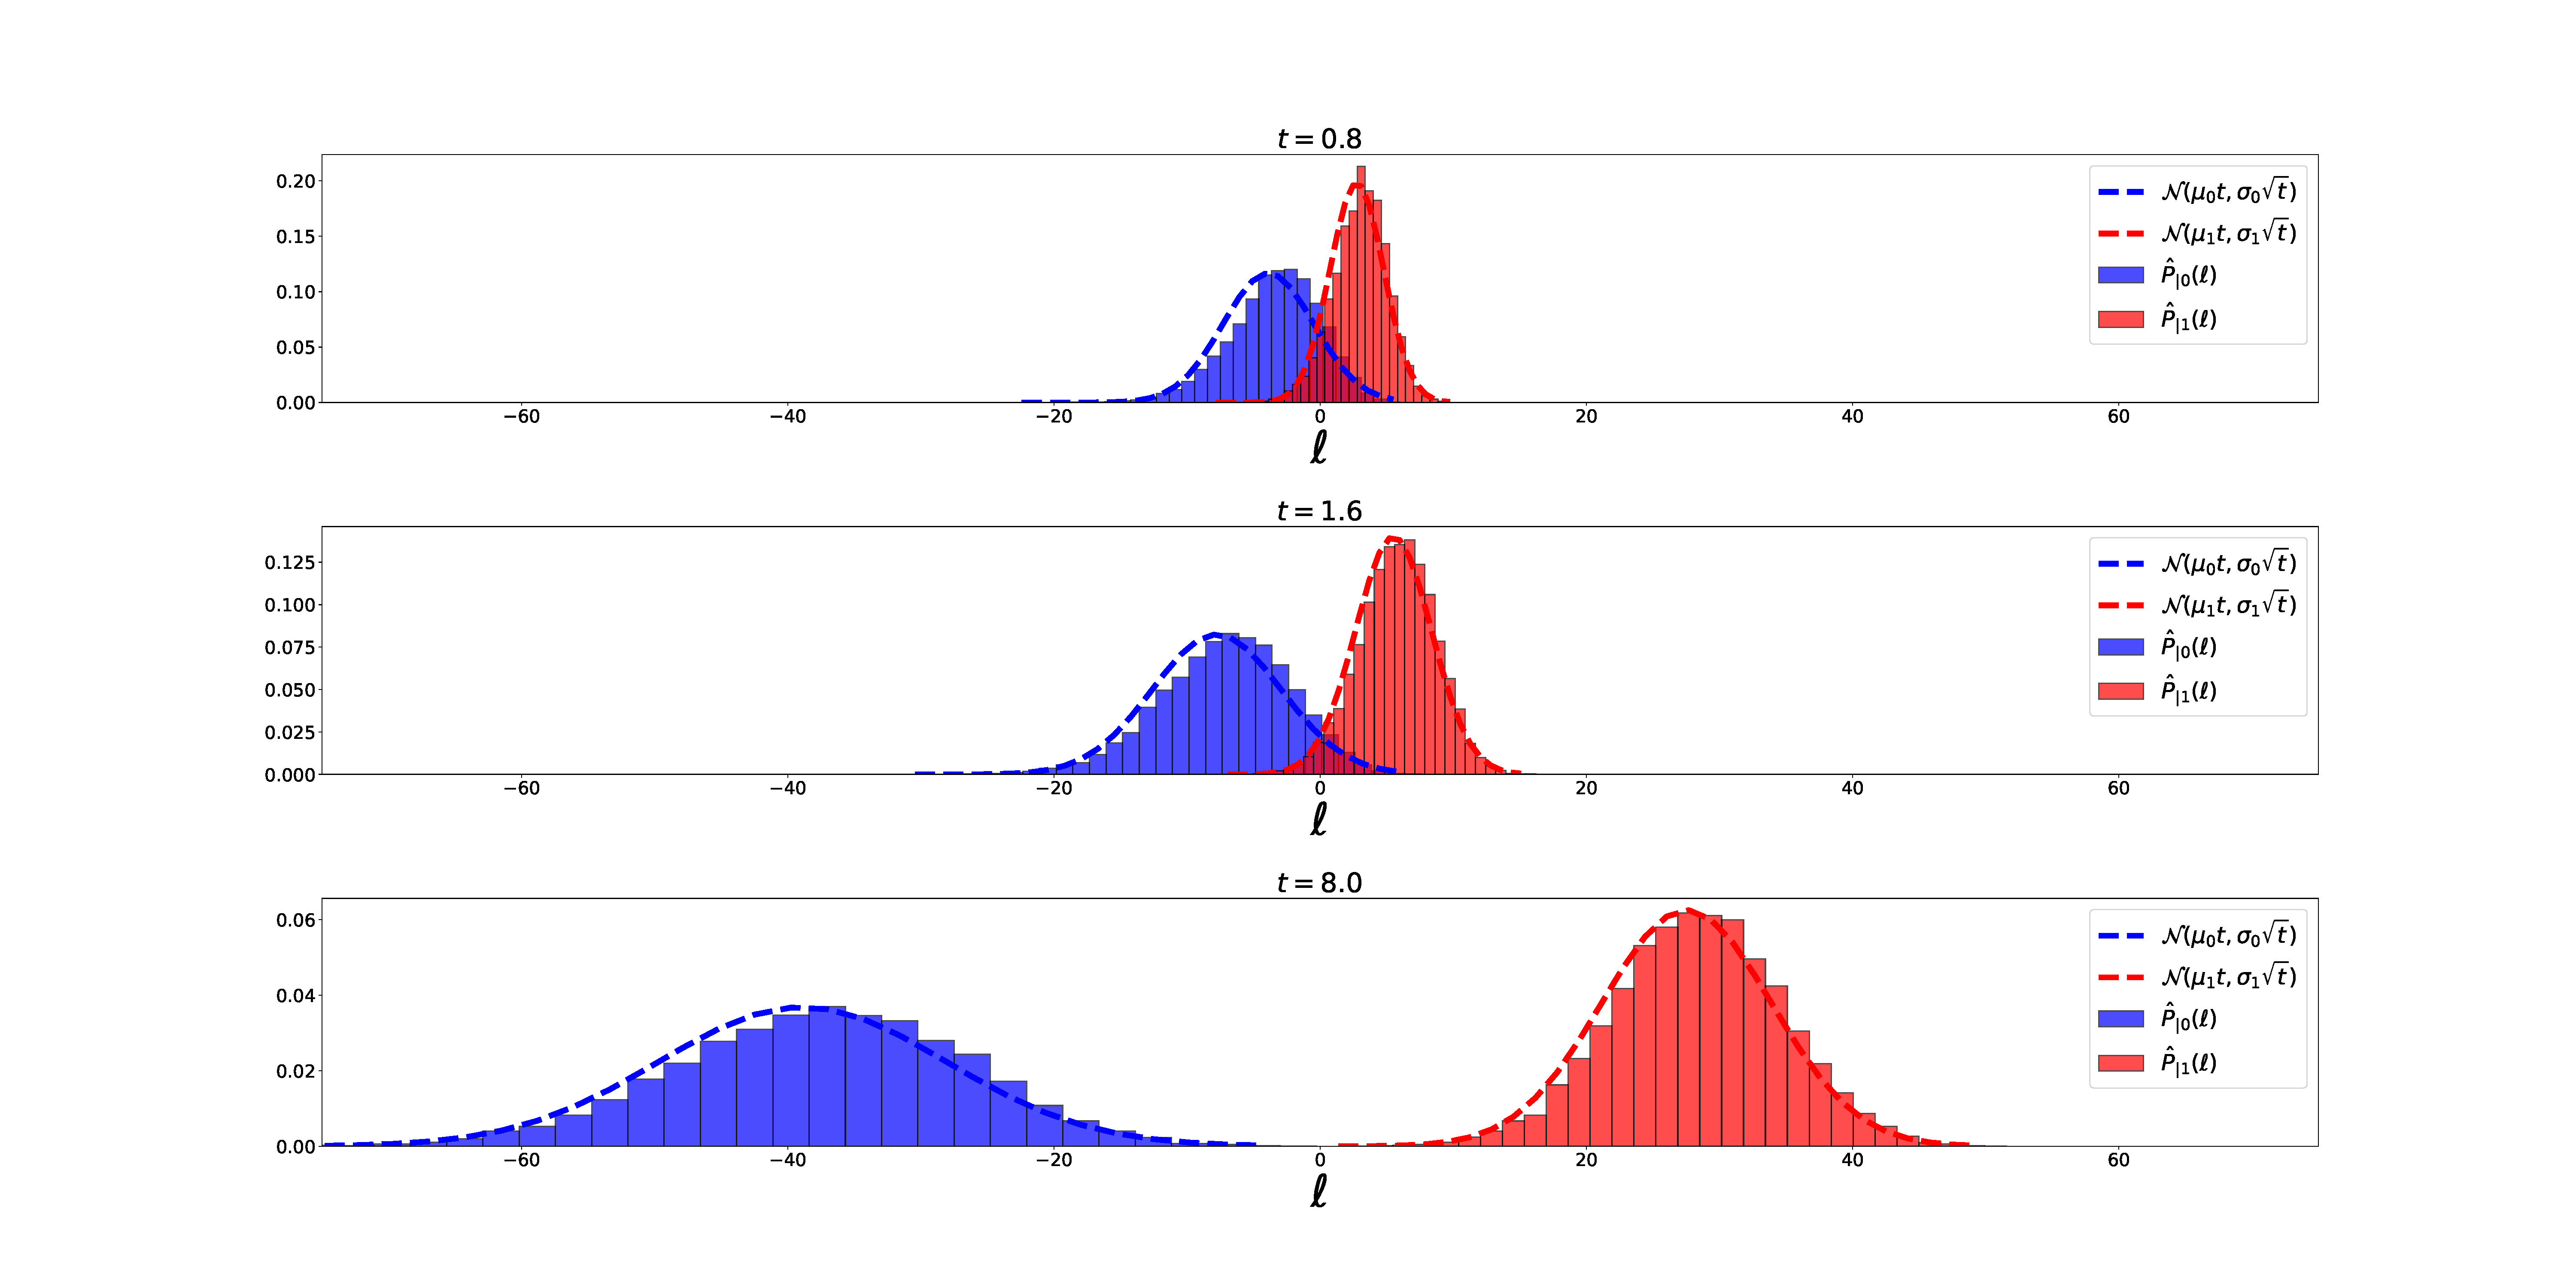
\includegraphics[width=1.\textwidth]{Figures/CMON/damp-discri/temp/histograms_10K.pdf}
    \caption{We show the distributions for the log-likelihood ratio at different times, for both hypothesis, computed over $2\cdot 10^{4}$ for the damping discrimination problem considered in this Section. Here, we have also plotted the distributions associated to the Gaussian model discussed in Sec.\ref{ssec:cmon_gaussian_model}.}
    \label{fig:histoell}
\end{figure}

The full probability distribution of $\ell_{t}$  can be seen in Fig.~\ref{fig:histoell}
where we give the histograms for $\ell_{t}$ at different time slices under each of the hypothesis. We note that for initial times, the distributions considerably overlap as expected ---with a low number of samples it is hard to distinguish the underlying model. As time progresses the two distributions separate from each other at a linear pace. We also observe that the distributions seem to be well approximated by a Gaussian. Indeed, from Eq.~\ref{eq:linealLog}, and the shape of the histograms in Fig.~\ref{fig:cmon_distributions_hidden} we might be tempted to say that $\DeltaXt$ concentrates around its mean $\mu_k$, and tends to a Gaussian with all cumulants of order 3 or higher scaling sub-linearly with $t$. Under such assumption, we could replace $\DeltaXt$ by $\mu_k$ in the dynamical evolution, and thus the process would reduce to an Orstein-Uhlenbeck process, discussed in Sec.~\ref{ssec:ito}. The solution of such process is a Gaussian distribution whose mean is drifted linearly in time and diffuses with a variance also proportional to $t$. As we will see in more detail bellow,
Sect. \ref{ssec:cmon_gaussian_model}, this intuition is only partially true.

\subsection{To be or not to be Gaussian}\label{ssec:cmon_gaussian_model}
The numerics and the heuristic argument given above seems to support that the distribution $P_k(\ell_{t})$ is indeed Gaussian. We begin this Section by providing a simple no-go theorem that shows $P_k(\ell_{t})$ cannot be Gaussian. We will then revisit again the heuristic argument and compute several quantities of interest under this, strictly speaking, wrong Gaussian assumption. We will show that the bulk of the distribution is correctly described by a Gaussian, but it completely fails to describe the tails (or large deviations).

\emph{No-go theorem for Gaussians}:
We will start by showing that assuming Gaussianity in both of the hypotheses implies $\mathbb{P}_{1}(\ell_{t}=x) = \mathbb{P}_{0}(\ell_{t}=-x)$, that is, the distributions are mirrored versions of each-other. To see this, we note that the following relation between the characteristic functions holds true:

\begin{align}
\chi_\ell(q-1)\equiv\mathbb{E}_{1}[e^{(q-1)\ell_{t}}] &= \int \mathcal{D}\Yt \; P_{1}(\Yt)  e^{(q-1)\ell_{t}}
=\int \mathcal{D}\Yt  \; P_{0}(\Yt) e^{\ell_{t}} e^{(q-1)\ell_{t}}=\nonumber\\
&=\int  \mathcal{D}\Yt \; P_{0}(\Yt)   e^{q\ell_{t}}=
\mathbb{E}_{0}[e^{q\ell_{t}}]\equiv \chi_\ell(q).
\end{align}
where we have used the fact that  $\ell(\Yt) = \log{\frac{P_1(\Yt)}{P_0(\Yt)}}$, to write
$e^{\ell}=\frac{P_1(\Yt)}{P_0(\Yt)}$  to perform a change of measure.
Now recalling that the characteristic function for a Gaussian distribution to be $\chi(q)= e^{(q\mu +\frac{q^2}{2}{\sigma^{2}})}$ we obtain \equ{(q-1)\mu_{1}+\frac{(q-1)^2}{2}\sigma_{1}^{2}  =-q\mu_{0}+\frac{q^{2}}{2}\sigma_{0}^{2}.}

Choosing now $q=0$, $q=1/2$ and $q=1$, we get the following identities: $(-)^{k+1}2\mu_{k}=\sigma_{k}^{2}$ and $2\mu_{1}+\sigma_{1}^{2}=-2\mu_{0}+\sigma_{0}^{2}$, which combined together give $\mu_{1}=-\mu_{0}$ and $\sigma_{0}^{2}=\sigma_{1}^{2}=2\mu_{1}$,
showing that $\mathbb{P}_{1}(\ell_{t}=x) = \mathbb{P}_{0}(\ell_{t}=-x)$. The latter condition that cannot be fulfilled by the model we study, since $\mu_0\neq -\mu_1$, as we can explicitly check from Eq.~\ref{eq:mukANAL} and clearly appreciate from Fig.\ref{fig:histoell}.
\emph{End of No-Go Theorem}

\bigskip

In the remaining of this Section we will see how far can we go analyzing the hypothesis testing scenario assuming the Gaussianity of $\mathbb{P}_{0}(\ell_{t})$, particularly because this allow us to get expressions for the weak errors under the deterministic setting, and to fully characterize the stopping-time probability distribution for the sequential state.

The central-limit theorem (CLT) guarantees that for \textit{i.i.d} random variables, the sample average will assymptotically normally distributed, centered in the mean value of the distribution and with a standard deviation that decreases as $\sim 1/\sqrt{N}$. If we consider the process
\eq{gausslog}{d\ell = (-1)^{k+1}\mu_k dt + \sigma_{k}dW_t,}
then we can readily find its associated probability distribution by recalling our discussion on OU-like processes from the previous Section and Sec.\ref{ssec:ito}. Such distribution reads
\eq{prob_gauss_log}{P_k(\ell) = \frac{1}{\sqrt{2 \pi \sigma_{k}^{2} t}}e^{\frac{(\ell + (-1)^{k+1} \mu_k t)^2}{2 \sigma_{k}^{2}t}}.}
From Eq.~\ref{eq:gausslog} and the CLT we expect the normalized variable $\frac{\ell_G}{t}$ to concentrate around its mean $(-1)^{k+1}\mu_k$ as $t\rightarrow\infty$, and \textit{approximating} its distribution by a Gaussian function around the mean-value should actually be \textit{always valid}, at least in the long-time regime. That is, we do expect the Gaussian approximation to hold under Eq.~\ref{eq:linealLog} around the mean-value of $\ell$: \textit{in the long-time regime, the probability distribution should look Gaussian in the bulk}. However, we do know that the Gaussian model should not hold, and we have already provided evidence of this in Fig.~\ref{fig:histoell}
and Fig.~\ref{fig:cmon_momentos}: while the distributions \textit{do} look Gaussian around their mean-value, the tails of the distribution are clearly not in correspondance with the Gaussian model.

In Sec.~\ref{ssec:1_hypo_testing} we have discussed two different approaches to the hypothesis testing scenario, namely the deterministic and the sequential one. We will now analyze such strategies for the system under consideration, when assuming that $\ell$ is normally-distributed.

\emph{Error probabilities for deterministic strategies.}
The deterministic tests consists on computing the value of $\ell(\Yt)$, for a fixed value of $t$, and making a decision for the undelying hypothesis based on its value. In this context, we will pay attention to the symmetric error, and thus the decision countour will be set at $\ell = 0$. Moreover, we will assume that the hypothesis are equally likely. Based on the log-likelihood ratio, the weak errors are defined as
\begin{align}\label{eq:cmon_errors_weak_gaussian}
 \alpha = P(\hat{h}_{1}|h_{0})&=\int_{0}^{\infty}P_{0}(\ell)d\ell \\
 \beta = P(\hat{h}_{0}|h_{1})&= \int_{-\infty}^{0} P_{1}(\ell)d\ell,\nonumber
\end{align}
where for compactness of notation we have defined $\ell=\ell_{t}$ at the given end time $t$ of the experiment.
%$$P_{k}(x,t)\equiv \int P(\ell_{t}(\mathcal{Y}_{t}) = x|\mathcal{Y}_{t})P(\mathcal{Y}_{t}|h_{k}) \mathcal{Y}_{t}.$$
Under the Gaussian model for $P_k(\ell)$, the errors can easily be computed and we get
\begin{align}\label{eq:cmon_errors_gaussian_formula}
\beta =\frac{1}{2}\left(1+\text{Erf}\left(\frac{\mu_{0} t}{\sqrt{2\sigma^2_{0} t}} \right)\right) \underset{t\rightarrow\infty}{\rightarrow} \sqrt{\frac{\sigma_{0}^{2} }{2\mu_{0} t }}e^{-\frac{\mu_{0}^{2}t}{2\sigma_{0}^{2}}},\\
\alpha =\frac{1}{2}\left(1+\text{Erf}\left(\frac{\mu_{1} t}{\sqrt{2\sigma_{1}^{2} t}} \right)\right)  \underset{t\rightarrow\infty}{\rightarrow} \sqrt{\frac{\sigma_{1}^{2} }{2\mu_{1} t }}e^{-\frac{\mu_{1}^{2}t}{2\sigma_{1}^{2}}}, \nonumber
\end{align}
In Fig.~\ref{fig:cmon_damping_err_weak} we compare these expressions with the numerical estimation of both type of errors, and for the symmetric one. Note that since the errors are computed from large deviation statistics, many quantum trajectories need to be simulated in order to have enough statistics to compute such quantities. As expected, the agreement between the Gaussian model and our numerics deprecates, particularly for long-times where we can differentiate the tails from the bulk.

\begin{figure}[t!]
    \centering
    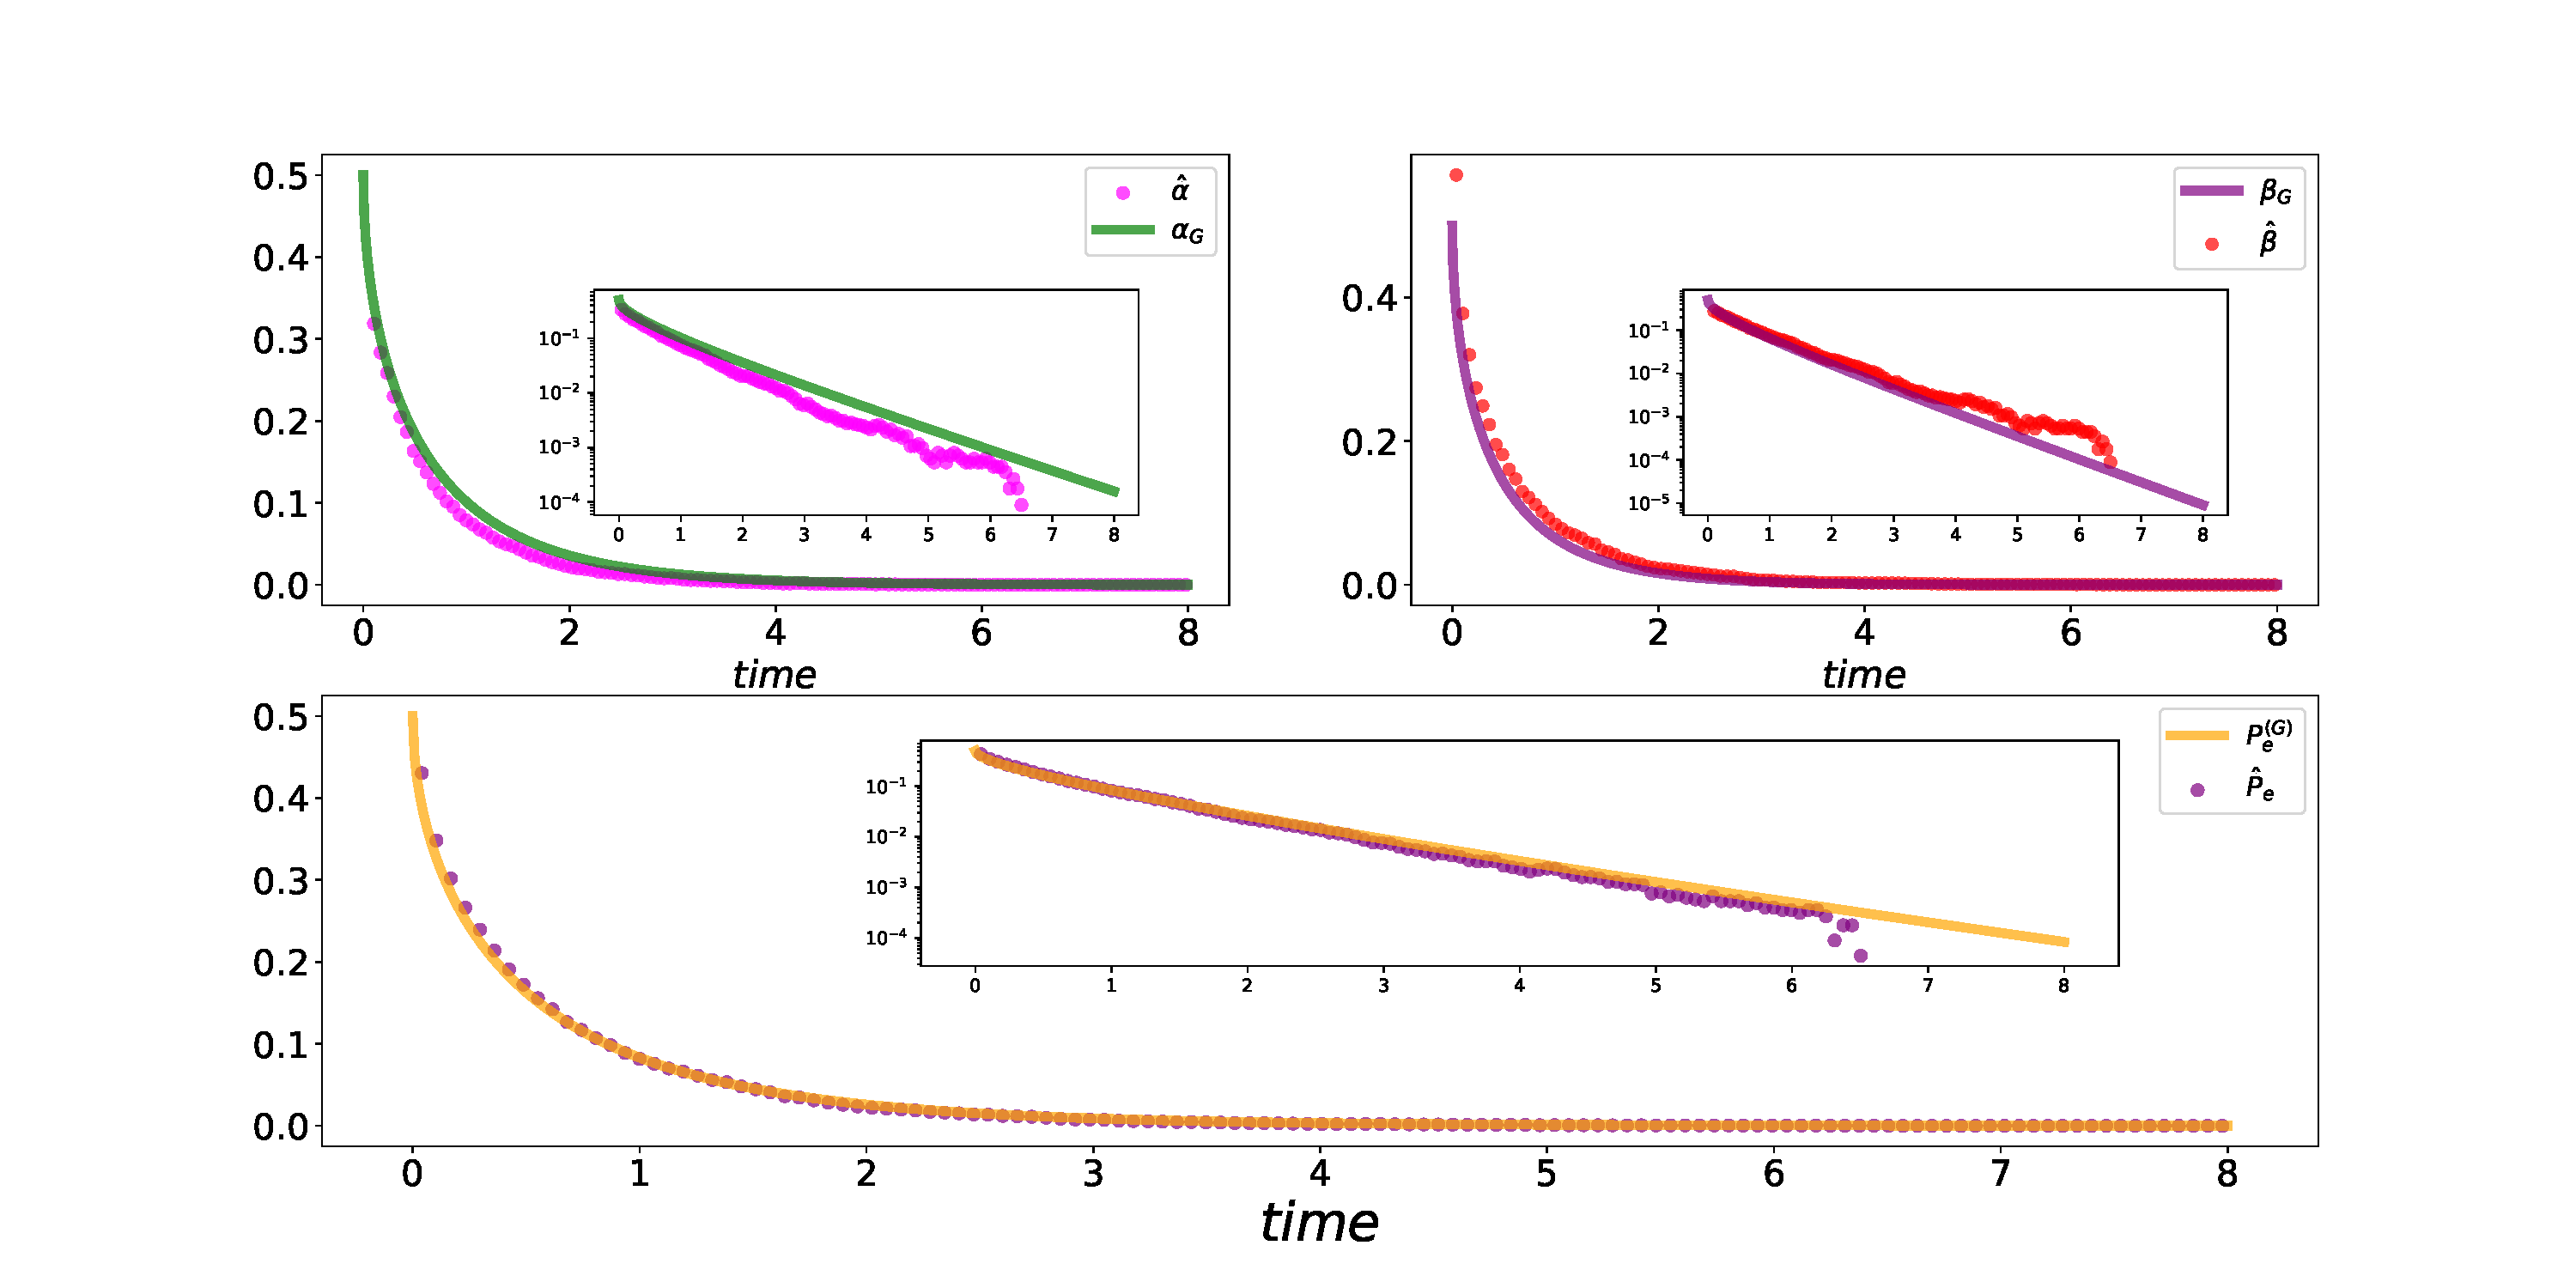
\includegraphics[width=1.\textwidth]{Figures/CMON/damp-discri/temp/deterministic_errors_time_gamma429.pdf}
    \caption{We show the weak errors computed for the deterministic test, and compare them with the expressions of Eq~\ref{eq:cmon_errors_gaussian_formula}, which are obtained by assuming that the distribution $P_k(\ell)$ is Gaussian.}
    \label{fig:cmon_damping_err_weak}
\end{figure}

\emph{Stopping time distribution for sequential hypothesis testing.}
Our result in Eq.\eqref{eq:waldcmon3} already gives the average stopping-time. However, we note that if $P_k(\ell)$ was a Gaussian distribution as per Eq.~\ref{eq:prob_gauss_log} then we would also fall in a new contradiction, since $\mu_k$ can only coincide with the relative entropy between the two Gaussian distribution only if $\mu_0 = \mu_1$\footnote{Recall that the relative entropy between two Gaussian distributions $\mathcal{N}_1(\mu_1, \sigma_1)$ and $\mathcal{N}_0(\mu_0, \sigma_0)$ is given by
\equ{D(\mathcal{N}_1||\mathcal{N}_0) = \log{\frac{\sigma_0}{\sigma_1}} + \frac{\sigma_1^2 + (\mu_1 -\mu_0)^2}{2 \sigma_0^2} - \frac{1}{2},}
which for the case under consideration ($\sigma_k = \sqrt{2\mu_k}$) reduces to
\equ{D(\mathcal{N}_1||\mathcal{N}_0) = \frac{1}{2}\log{\frac{\mu_0}{\mu_1}} + \frac{2 \mu_1 + (\mu_1 - \mu_0)^2}{4 \mu_0}- \frac{1}{2}.}
}.

However, if we ignored all of the issues pointed out above --- for instance, assume that the drifts do only differ slightly --- then an expression for the full stopping-time probability probability distribution can be obtained. Thus, we will consider an stochastic process
\eq{dellgauss}{d\ell_t = \mu dt + \sigma dW_t,}
whose probability distribution at time $t$ will be denoted by $P(\ell_{l})$, and is understood as the probability that the state takes the value $\ell$ at time $t$.

Assuming that the SPRT eventually stops, \textit{i.e.} $\ell$ eventually exits the undecision region $\Omega$, then the stopping-time probability distribution $P(\tau=t)$, \textit{i.e.} the probability that the stopping time takes a value of $t$ can be written in terms of its cumulative distribution as
\eq{ptau}{P(\tau = t) = -\frac{d}{dt} P(\tau>t) = -\frac{d}{dt} \int_t^{\infty} P(\tau) d\tau.}
Now, the probability that the stopping-time is larger than $t$ is given by the total probability of finding the stochastic process $\ell$, at times smaller or equal to $t$, inside the undecision region $\Omega$:
\equ{P(\tau>t) = \int_{-a_0}^{a_1} \mathcal{P}(\ell, t) d\ell.}
Note our slight abuse of notation: we understand $\int d\ell$ as an integral over measurement record realizations $\mathcal{Y}_t$ that lead to $\ell(\mathcal{Y}_t) = \ell$. Moreover, in the last integral we assume that the values of $(\ell,t)$ we are integrated over have not reached the decision boundary $\Omega$ for times smaller than $t$, thus $\mathcal{P}(\ell, t)$ is deemed \textit{survival probability}; due to this fact we will use the $\mathcal{P}$ notation for this process. This quantity can be obtained as a solution of the Fokker-Planck equation (plus absorbing boundary conditions), as per
\begin{align}
\partial_t \mathcal{P}(\ell,t) &=  -\mu \partial_\ell \mathcal{P}(\ell,t)+ \frac{\sigma^2}{2} \partial^2_\ell \mathcal{P}(\ell,t),\\
\mathcal{P}((\ell,t) \notin \Omega) &= 0.
\end{align}
The initial condition for this problem is given by $\int_{\Omega} P(\ell,0)d\ell = 1$. Combining the above equations and using the Leibniz integral rule, we obtain
\equ{P(t) = \frac{\sigma^2}{2} \partial_\ell \mathcal{P}(\ell_t)|_{\ell=a_0}^{a_1}  + \frac{\sigma^2}{2}\int_{a_0(t)}^{a_1(t)} \Big(\dot{a}_0 \partial_{a_0(t)} + \dot{a}_1\partial_{a_1(t)}\Big) \mathcal{P}(\ell,t) d\ell,}
where we have account for the possibility that the decision boundaries change in time. In turn, if we now change of variables as $l_{t} = \ell_t - \mu t$, then $\Omega$ becomes time-depentend as $\Omega(t) = [a_0(t),a_1(t)]$ with $a_i(t) = a_i + \mu t$. The Fokker-Planck equation associated with the process $l$ is symmetric under reflection operations of the form $l\to 2\beta-l$ with $\beta \in \mathbb{R}$, allowing for the use of the image charge method to find an explicit solution in the form of an infinite series for the survival probability $P(\ell,t)$:
\begin{align}\label{eq:charge_seriess}
\mathcal{P}(\ell,t) &=\bar{P}(\ell,t)\\
&+\sum_{n=1}^{\infty}\Big\{ \bar{P}(2n(a_{1}(t)-a_{0}(t))+\ell,t) -  \bar{P}(2{n}a_{0}(t)-2(n-1)a_{1}(t)-\ell,t) \nonumber\\ \nonumber
&+\bar{P}(2n(a_{0}(t)-a_{1}(t))+\ell,t) - \bar{P}(2{n}a_{1}(t)-2(n-1)a_{0}(t)-\ell,t)\Big\}
\end{align}
where
\begin{align}\label{eq:Pheat}
\bar{P}(\ell,t) &= \frac{1}{\sqrt{2\pi \sigma^2 t}} e^{-\frac{\ell^{2} }{2 \sigma^2 t}}
\end{align}
is the solution of the differential problem $\partial_{t}\mathcal{P}(l,t)= \frac{\sigma^2}{2} \partial_{l}^{2}\mathcal{P}(l,t)$ with initial condition $\mathcal{P}(l,0)=\delta(l)$. Substituting Eq.~\eqref{eq:charge_seriess} in Eq.~\eqref{eq:ptau}, and after some (tedious) algebra and keeping only the lowest-order terms associated with the limit $A = \text{min}(|a_0|, |a_1|) \rightarrow \infty$, \textit{i.e.} very low errors which is also associated to long-times, we get that the stopping-time probability distribution is an inverse-gaussian (or Wald distribution):
\begin{align}
P(t) = \frac{|a_k|}{t^{3/2}\sqrt{2\pi \sigma^2_k}}e^{-\frac{(a_k + (-1)^{k+1} \mu_t t)^{2}}{2 \sigma^2_k t}},
\end{align}
where we have taken into account that hypothesis $k$ is the underlying one when taking the limit.

While the solution for the process in Eq.~\ref{eq:dellgauss} corresponds to a drifted and diffused Gaussian distribution whose expression is explicited in Eq.~\ref{eq:prob_gauss_log}, we are now interested in the probability that a trajectory drawn from such Gaussian distribution hits the decision boundary $\Omega = [-a,a]$. Since the mean of the $\ell$ increases as $\mu t$, and its standard deviation as $\sigma \sqrt{t}$, the resulting projection of such probability into the line $\ell=a$ (for hypothesis $k=1$) leads to a tilted distribution, as illustrated in Fig.~\ref{fig:cmonwald} which is known as the Wald distribution, and reads
\equ{P(\tau) = \frac{a}{\sqrt{2 \pi \sigma^2 t^3}} e^{-\frac{(a - \mu t)^2}{2 \sigma^2 t}},}
where $\tau$ stands for the time at which the $\ell_\tau = a$, \textit{i.e.} the stopping time. We note that a similar distribution is obtained for $k=0$.  Moreover, the mean of this distribution is
\eq{meanWALDdisto}{\expect{\tau} = \frac{a}{\mu},}
and we note that this coincides with the Wald identity in Eq.~\ref{eq:waldcmon3} (see also Eq.~\ref{eq:sptrWaldsimple}) for large values of $a\sim\log\epsilon$.

From our discussion regarding the validity of the Gaussian distribution, we do expect the Wald distribution to match our numerics close to the bulk, and this is shown in Fig.~\ref{fig:stop_time_distro}. While the agreement is particularly good for the bulk of the distributions, we note that the tails are quite off, particularly for $k=0$, for which the drift is higher.

\begin{figure}[t!]
    \centering
    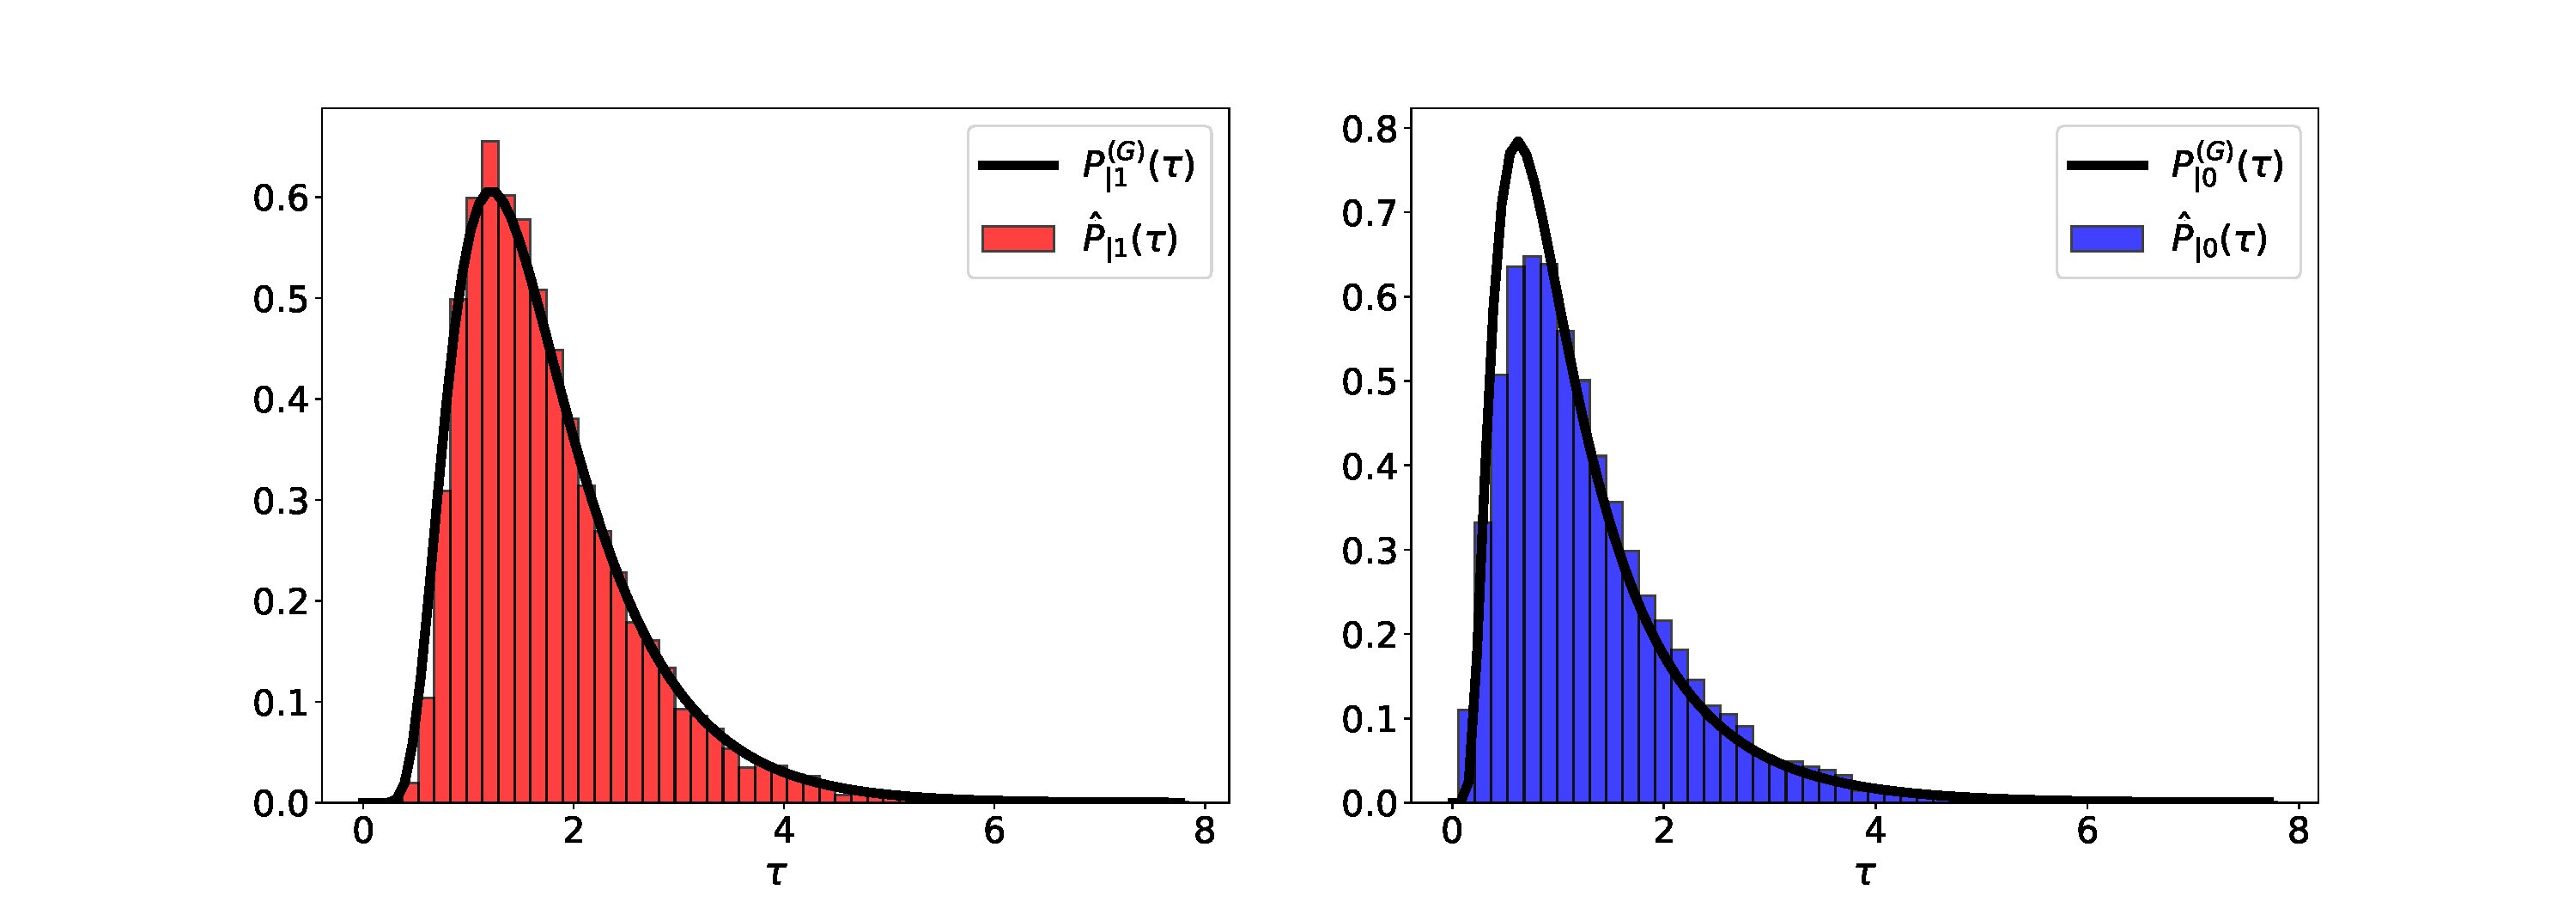
\includegraphics[width=1.\textwidth]{Figures/CMON/damp-discri/temp/stopp_time_b6_gamma429_both.pdf}
    \caption{We show the stopping time probability distributions, under both hypothesis, obtained numerically by carrying out the SPRT on 20K trajectories for the damping discrimination problem under consideration. Here, we have chosen a value of $a=6$, \textit{i.e.} $\epsilon\sim0.0025$.)}
    \label{fig:stop_time_distro}
\end{figure}


\subsection{Joint system evolution as an OU-process}\label{ssec:oucoupled}
We have already shown that $\mathbb{E}_{k}\Big[||\DeltaXt||^2\Big]= \mu_k t$, and we will next outline an alternative method to compute its variance, which scales lineary with time as $\text{Var}_k\Big[||\DeltaXt||^2\Big]= \sigma^2_k t$. The fact that that $\ell$ is not compatible with a Gaussian distribution can be understood from the back-action term due to the measurement record, which couples the dynamical equations for the two hypothesis. Having this in mind, it is convenient to treat the problem in an extended vector space where the state of the system is defined as $\mathbf{X}_{t}=(\rbar_{0}(t),\rbar_{1}(t))^{T}$ and $\SigmaJoint{t} =\cov_{0}(t)\oplus\cov_{1}(t)$ whose evolution is given by
\begin{align}
d\mathbf{X}_{t} &=  (\mathcal{A} -\chi(\SigmaJoint{t}) \Pi_{k} \mathcal{C}) {\mathbf{X}}_{t} dt +\chi(\Sigma) d\mathbf{w}_{t}\nonumber\\
\dot{\SigmaJoint}_t &= \mathcal{A} \SigmaJoint_t+\SigmaJoint_t \mathcal{A} +\mathcal{D}-\chi(\SigmaJoint_{t})\chi(\SigmaJoint_{t})^{T}
\end{align}
with $\mathcal{A}=A_{0}\oplus A_{1}$, $\mathcal{C}=C\oplus C$ and $\mathcal{D}= D_{0}\oplus D_{1}$, $\chi(\SigmaJoint_{t}) := \SigmaJoint_{t} \mathcal{C}^T +\tilde{\Gamma}$, $\tilde{\Gamma}= \Gamma_{0}\oplus\Gamma_{1}$
and
\begin{align*}
  \Pi_{0}=\begin{pmatrix}
    0 & 0\\
  \one & -\one
   \end{pmatrix},
   \hspace{0,5cm}
   \Pi_{1}=\begin{pmatrix}
  \one & -\one\\
    0   &   0
   \end{pmatrix}
  \end{align*}
with $k$ denoting the hypothesis under which the signal $\mathcal{Y}_{t}$ is generated (\textit{i.e.} $k=0,1$). Under this notation, the evolution for the log-likelihood ratio reads:
\begin{align}
d\ell(\mathcal{Y}_{t|\theta_{k}},t) =\frac{(-)^{k+1}}{2} |\mathbf{\Delta}^{T}\mathcal{C}{\mathbf{X}_{t}} |^2 dt + \mathbf{\Delta}^{T}\mathcal{C}{\mathbf{X}_{t}} d\mathbf{w}_{t}
\end{align}
with $\mathbf{\Delta}^{T}= (1,-1)^{T}$. Under the assumption that the evolution for the covariance admits a stationary solution $\SgmJointSt= \sigma_{0}\oplus\sigma_{1}$, the probability distribution of $\mathbf{X}_{t}$ is assymptotically given by:
\begin{equation}
P_{st,k}(\bold{X})=  \frac{1}{(2\pi)^{n/2} \text{det}[\bomega]^{1/2}}\exp{(-\frac{1}{2}\bm{X}^{T}\bomega^{-1}\bm{X}})
\end{equation}
where $\bomega$ is the solution of the Lyapunov equation $(\mathcal{A}-\chi(\Sigma_{t})\Pi_{k}\mathcal{C})\bomega+\bomega(\mathcal{A}-\chi(\SgmJointSt)\Pi_{k}\mathcal{C})^{T}=\chi(\SgmJointSt)\chi(\SgmJointSt)^T$\footnote{This equation arises from a generalization of the OU-process discussed in Sec.~\ref{ssec:ito} to multivariable systems, and we refer the interested reader to Ref.~\cite{gardiner2004handbook} for more details.}
Using this notation, we can express the assymptotic behaviour for the expected value of $\ell$ as
\begin{align}\label{eq:dlimit}
\underset{t\to \infty }{\text{lim }}\frac{\mathbb{E}_{k}[d\ell(\mathcal{Y}_{t})]}{t} &= \frac{(-)^{k+1}}{2}\mathbb{E}[ |\mathbf{\Delta}^{T}\mathcal{C}\mathbf{X}|^{2}] \nonumber\\
&= \frac{(-)^{k+1}}{2}\tr{\mathcal{C}^{T}\mathbf{\Delta\Delta}^{T}\mathcal{C}\bomega}.
\end{align}
From here, we can insert the formal solution of $\mathbf{X}_{t}$ to get
\begin{equation}
\mathbf{\Delta}^{T}\mathcal{C}\mathbf{X}_{t} = \mathbf{\Delta}^{T}\mathcal{C}e^{(\mathcal{A}-\chi(\SgmJointSt)\Pi_{k}\mathcal{C})(t-t_0)}\mathbf{X}_{t_{0}} + \chi(\SgmJointSt) \int_{t_{0}}^{t} \mathbf{\Delta}^{T}\mathcal{C} e^{(\mathcal{A}-\chi(\SgmJointSt) \Pi_{k}\mathcal{C}) (t-\tau)} \dwtau.
\end{equation}
Finally, by defining
\begin{align}
g(t-t_{0}) &= \mathbf{\Delta}^{T}\mathcal{C}e^{(\mathcal{A}-\chi(\Sigma_{st})\Pi_{k}\mathcal{C})(t-t_{0})}\mathbf{X}_{t_{0}} \nonumber\\
f(t-s) &= \mathbf{\Delta}^{T}\mathcal{C}\, e^{(\mathcal{A}-\chi(\Sigma_{st})\Pi_{k} \mathcal{C})(t-s)} \chi(\Sigma_{st})\mathbb{Q}
\end{align}
with $\mathbb{Q}= (1,1)^{T}$, we arrive to an assymptotic expression for the mean and covariance of $\ell$:
\begin{align*}
&\mathbb{E}_{k}[\ell_{t}] =
\underset{t\rightarrow\infty}{\text{lim}} \frac{(-)^{k+1}}{2}\left\{\left(\int_{t_{0}}^{t}g(\tau-t_{0})d\tau\right)^{2} -\int_{t_{0}}^{t}d\tau \int_{t_{0}}^{\tau} f(\tau-s)^{2}ds\right\} \nonumber\\
&\mathbb{E}_{k}[\ell_{t}^{2}]-\mathbb{E}_{k}[\ell_{t}]^{2} =
\lim_{t_{0} \to -\infty } \int_{t_{0}}^{t}d\tau\int_{t_{0}}^{\tau}f(\tau-s)^{2}ds \nonumber\\
&-2\int_{t_{0}}^{t}d\tau_{1}\int_{t_{0}}^{\tau_{1}}d\tau_{2}f(\tau_{1}-\tau_{2})\int_{t_0}^{\tau_{2}}dsf(\tau_{1}-s)f(\tau_{2}-s)\nonumber\\
&+\int_{t_{0}}^{t}d\tau_{1}\int_{t_{0}}^{\tau_{1}}d\tau_{2}\left(\int_{t_{0}}^{\tau_{2}}f(\tau_{1}-s)f(\tau_{2}-s)ds\right)^{2}.
\end{align*}
Overall, this constitutes an alternative approach to compute the first two moments of $\ell$, and for the damping discrimination case-study we can readily check that the above expression matches Eq.~\ref{eq:mukANAL}. Moreover, in Fig.~\ref{fig:cmon_momentos} we have compared our numerics with the analytical expressions that we get using these formulae for the damping discrimination case, for both the average and variance of $\ell$. As we can see, after a trancient time, a good agreement can be observed. We remark that numerical errors associated to the integration routine lead to considerable computational-resources usage. Here, we have used the Python package \texttt{sdeint}~\cite{sdeint} which implements an order 1 strong-convergence stochastic Runge-Kutta method, introduced in Ref.~\cite{robler}\footnote{Whereas strong convergence stands for the average error commited per time-step, the \textit{weak} convergence refers to the error of the mean values obtained by averaging out the integrated trajectories. The order is measured in terms of $dt$, for instance Euler algorithm has order $\frac{1}{2}$.}




\subsection{Deterministic vs Sequential}
While we have discussed the validity of the Gaussian model for $\ell$, let us note that the expected time required to reach a certain threshold for the error probability is $4$ times lower in favour of the SPRT. This can be seen from the asymptotic behaviour of the asymmetric errors in Eq.~\ref{eq:cmon_errors_gaussian_formula}, \textit{i.e.} we obtain $\log{\alpha_k}\sim-\frac{\mu_k t}{4}$, with $\alpha_0 = \alpha$ and $\alpha_1 = \beta$.

For the general case, we do expect an advantage in favour of the sequential, but (for the moment) we rely on numerical methods to compute the advantage. In Fig.~\ref{fig:comparison} we compare the average time required by the SPRT to reach a given error threshold for the symmetric error probability, as given by Eq.~\ref{eq:weakErrorsSPRT}, with that of deterministic test. For the latter, we compute the empirical probability of error for several times, and use interpolation to find the time at which a given mean error is reached. In both cases, we compare with the theoretical models, namely the rigorous results for the sequential case, and the calculations based on the Gaussian approximation for the deterministic case.

\begin{figure}[t!]
    \centering
    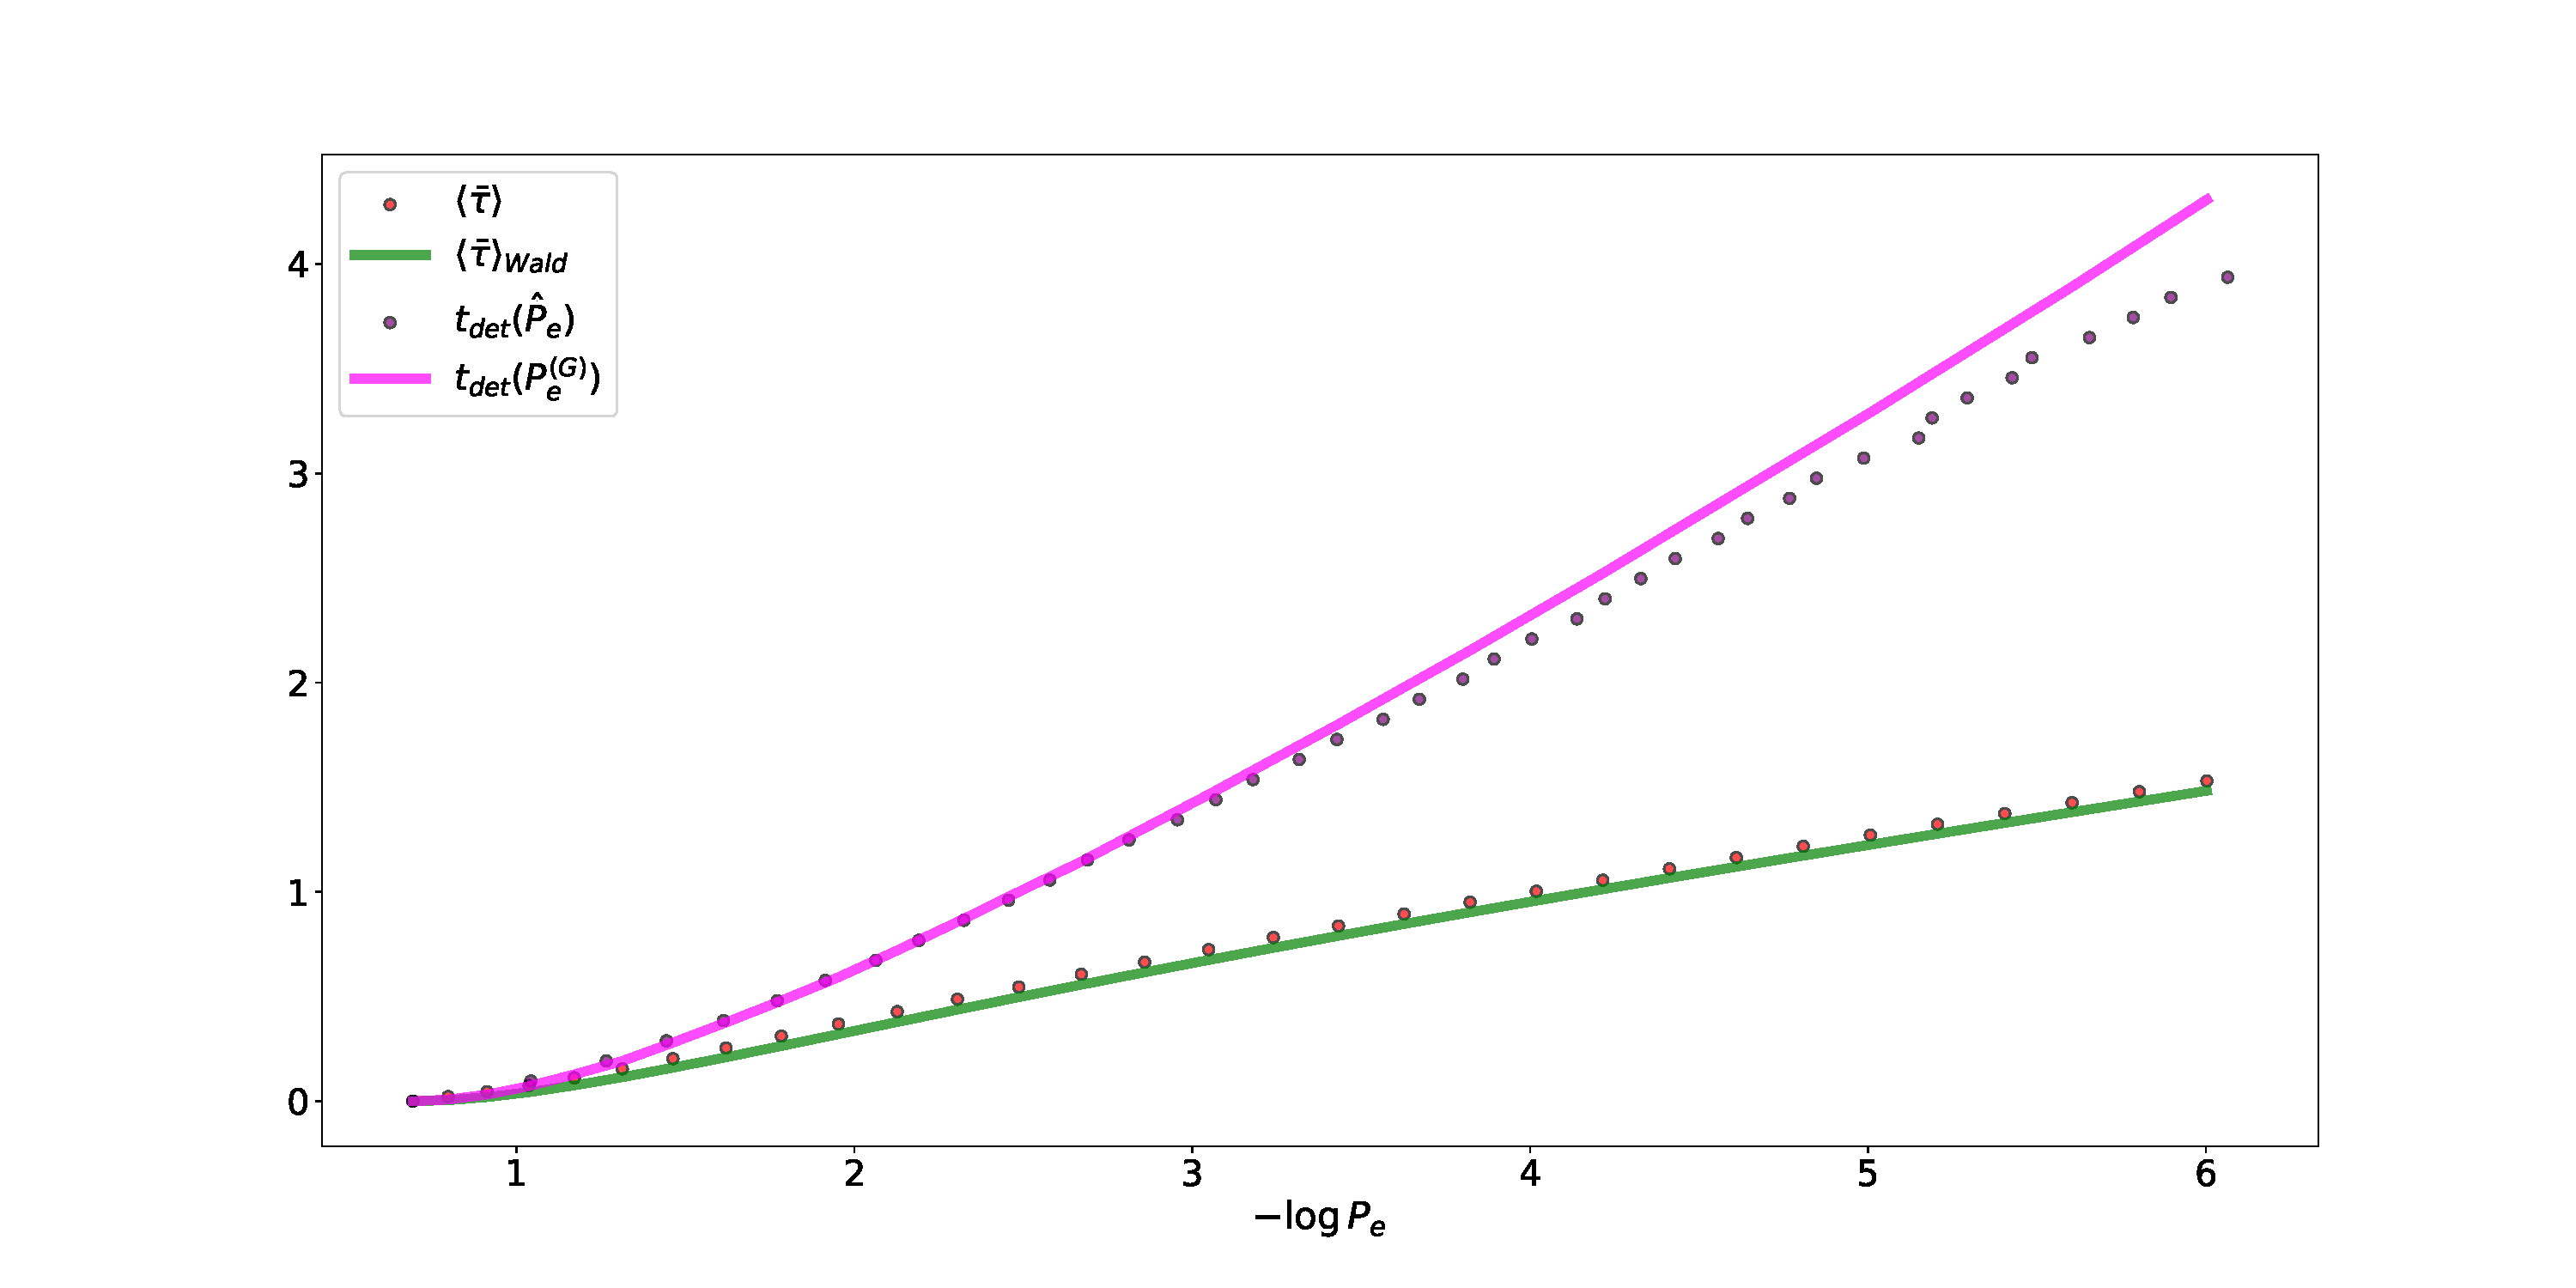
\includegraphics[width=1.\textwidth]{Figures/CMON/damp-discri/temp/fig9.pdf}
    \caption{We compare the performance of the sequential test against the deterministic one, in terms of the average time that takes the test to reach a certain error threshold. In the deterministic case, we invert the Gaussian model for the symmetric error, to get the desired time. This was done by interpolating the time that the superposition of Lorentzian distributions requires to value the pre-defined error threshold $P_e$, as given when fixing $\epsilon$ in Eq.~\ref{eq:weakErrorsSPRT} and computing $\frac{1}{2}(\alpha + \beta)$. Such a Gaussian model is also compared with our numerics, and in this plot we show the numerical value of the symmetric error probability in the deterministic case ($x$ axis), at the different times it was computed for ($y$ axis). For the sequential test, we show the average stopping time as a function of $P_e$, and compare this with the quantity that Wald identity predicts.}
    \label{fig:comparison}
\end{figure}

To sum up, we have introduced a sequential hypothesis testing approach to the discrimination between two physical models in continuously-monitored systems, showing a clear advantage of the latter as compared to the deterministic test. While we have focused on the damping-rate discrimination case, since some analytical insight can be gained, let us stress that the sequential approach is ought to be taken not only for a different set of parameters in the (quantum) Gaussian model for the optomechanical system, but also for general stochastic evolutions.


\subsubsection{Frequency discrimination}
\begin{figure}[t!]
    \centering
    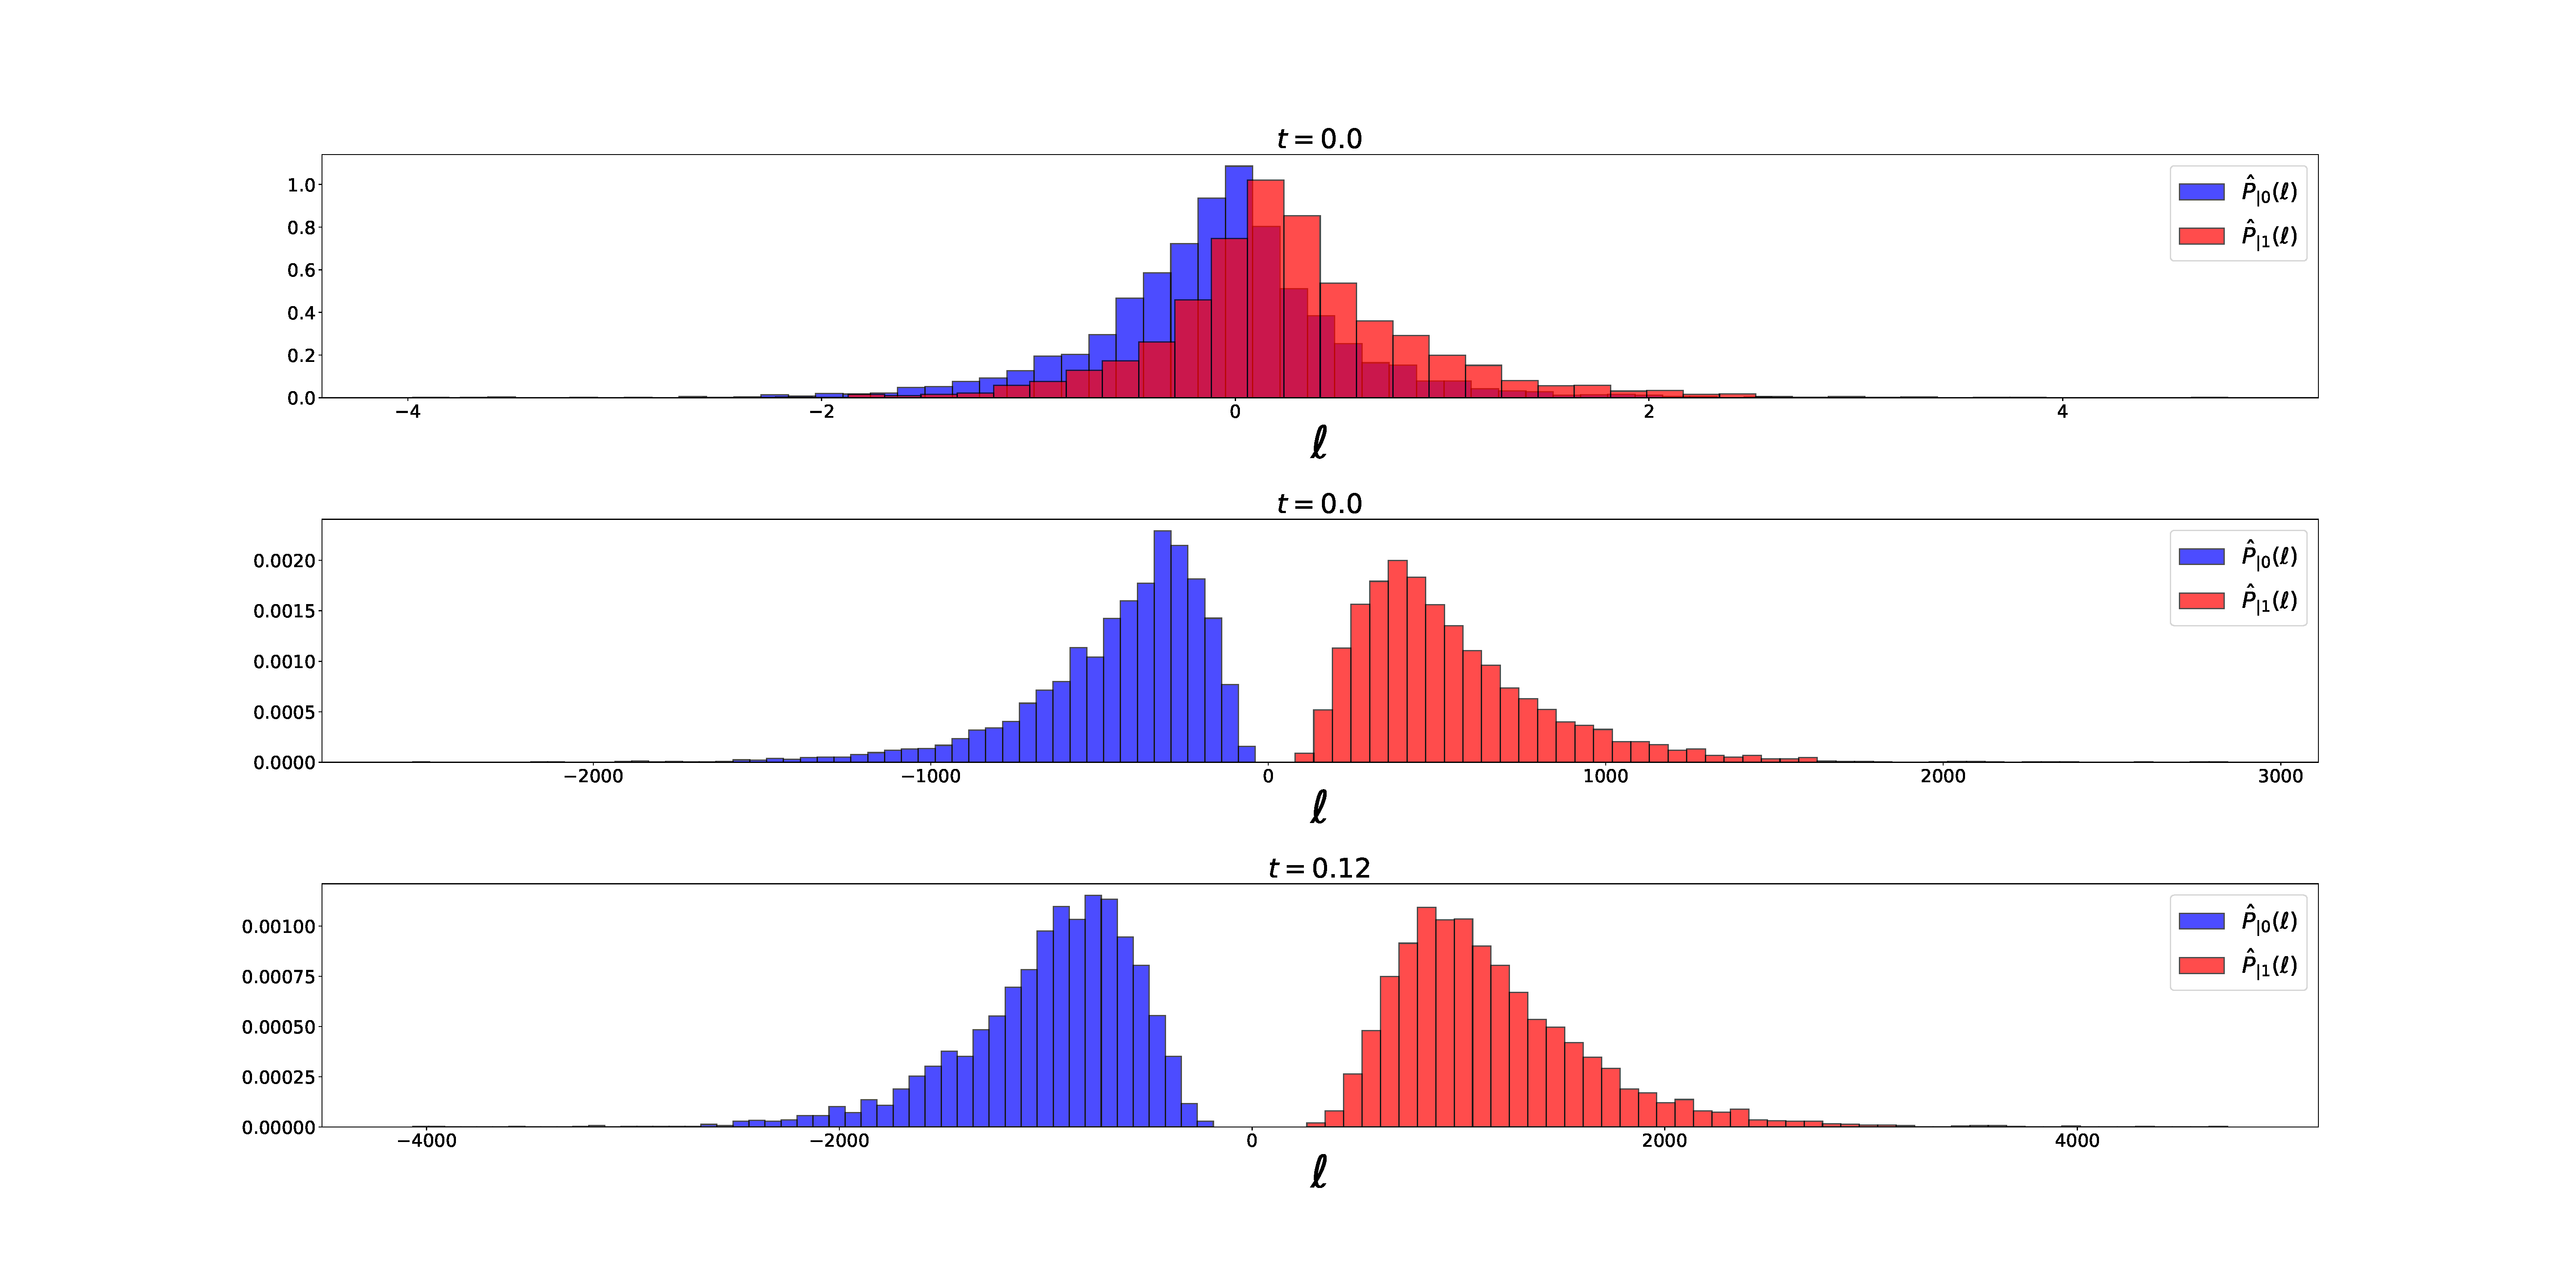
\includegraphics[width=1.\textwidth]{Figures/CMON/freq-discri/histo_freqs.pdf}
    \caption{We show the distributions of the $\ell$ for the frequency discrimination problem, where $\omega_0 = 10^4 Hz$ and $\omega_1 = 1.1 \cdot 10^4 Hz$, $\eta = n = 1$ and $\kappa=1000 Hz$. The reason we take such a high value of $\kappa$ is to aid with the computing resources and time simulation. The results are shown for $10^{4}$ quantum trajectories.}
    \label{fig:freq_histo}
\end{figure}

To complement our numerical study of the sequential hypothesis test in continuously-monitored systems, we here study the case of frequency discrimination. In Fig.~\ref{fig:freq_histo} we show how the probability distribution of $\ell$ looks for the two hypothesis, each associated to a different value of the mechanical-mode frequency. We observe that, for the times under consideration, the distributions are clearly not Gaussian. Note that here we are not analyizing the data in the rotating-frame, since the frequency is unknown. One of the consequences of this fact is that a transcendental equation for the stationary value of the covariance matrix arises in Eq.~\ref{eq:cmon_LINEALSYSTEM}, and thus little can be done analytically-wise when aiming to obtain the values of the drift and difussion for $\ell_t$.

Following a similar analysis than in the damping discrimination case, in Fig.~\ref{fig:compa_freq} we compare the sequential and deterministic strategies' performance, showing also a clear advantage in favour of the former.
\begin{figure}[t!]
    \centering
    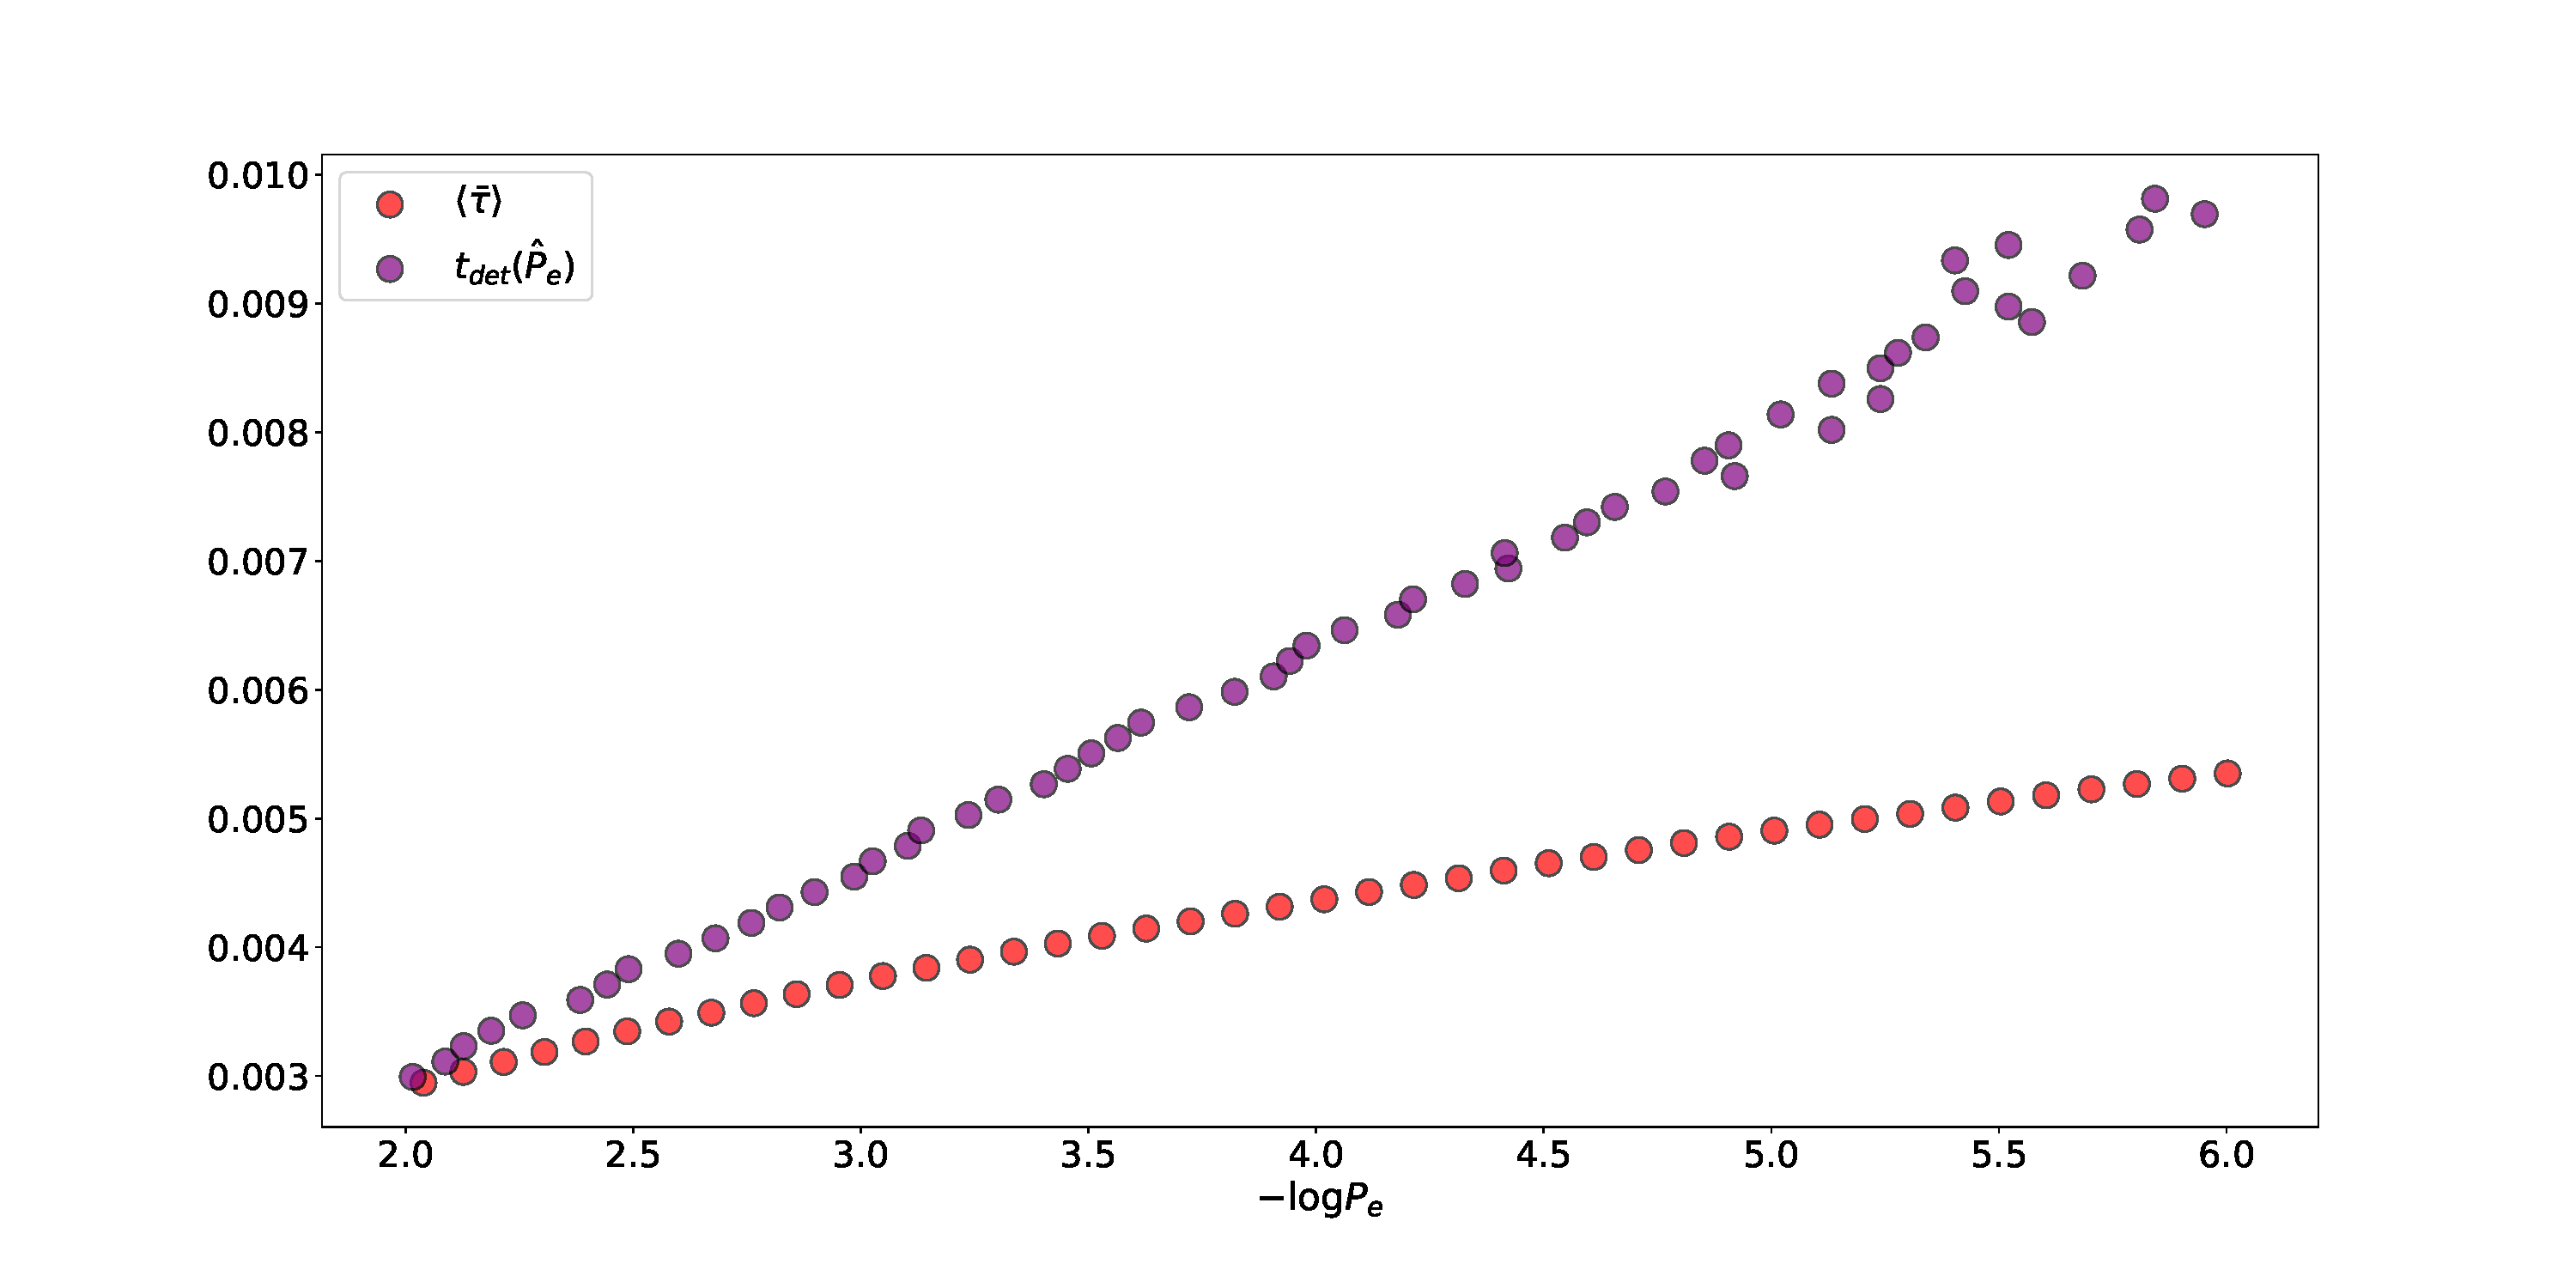
\includegraphics[width=1.\textwidth]{Figures/CMON/freq-discri/error_comparison_short_times_nicer.pdf}
    \caption{Here we show the same comparison between the performance of both discrminiation strategies (sequential vs. deterministic), similarly to Fig.~\ref{fig:comparison}, but for the frequency discrimination case.}
    \label{fig:compa_freq}
\end{figure}

\section{Parameter estimation $\&$ continuously-monitoring}\label{sec:cmonEST}
In the previous Section we have discussed how to discriminate between two different phyiscal models, and provided strong numerical evidence in favour of the sequential strategy. Moreover, in the examples we have considered the damping discrimination case, and the analytical results we obtained hinge on the fact that the mechanical-mode's frequency is known. By the end of the previous Section we discussed the case in which such value is discerned between two possible candidates. However, in general we need to estimate this quantity, what reduces to a different problem in statistical-inference, namely the (classical) parameter estimation discussed in Sec.~\ref{ssec:1_stinf_estimation}.

In this Section we will comment on a work in progress, which consists on estimating a parameter encoded in a physical system that is being continuously monitored. Our preliminary results consist on implementing the maximum-likelihood with the automatic-differentiation machinery, and the ultimate goal of this (ongoing) project is that of machine-learning the \textit{dynamics} of a continuously-monitored system. By this we understand asking the machine-learning to provide a set of dynamical equations based solely on the observed data, similar to the proposals of Ref.~\cite{sindy} (though taking noise and back-action terms into account). The latter can be useful when aiming to model external signals, and we will here study simple examples that enter in the evolutino as external forces \textit{e.g.} drives.

\subsection{The spectral power and the Lorentizan fit}\label{ssec:lorentzian}
To infer the value of the frequency, it is customary to fit a Lorentizan function to the spectral power of the signal. The power spectrum of a stationary stochastic process, say a quadrature of a mode, $x_{t}$, is the Fourier transformed of its autocorrelation function, \textit{i.e.} $S(\omega) = \int_{-\infty}^\infty dt' e^{\ii \omega t'} \langle x_{t}x_{t+t'}\rangle$. For a damped oscillator system as the one described in Eq.~\ref{eq:cmon_LINEALSYSTEM}, such quantity is given by a Lorentzian peaked at the mechanical-mode frequency as per
\equ{S(\omega) \sim A \frac{\gamma}{(\omega - \omega_m)^2 + \frac{\gamma}{2}}, }
where $A$ is a constant factor related to bath's temperature~\cite{clerckintroductionnoise}. Here, we are interested in how to estimate a physical parameter out of a \textit{single} quantum trajectory, whose access is granted via the measurement record. Whence, we consider a single process realization (and not the average), and replace the hidden state $\mathbf{r}_{t}$ by the measurement record $d\mathbf{y}_{t}$, given by the homodyne measurement that projects onto the $q$ quadrature of the hidden state (\textit{i.e.} we are not considering the rotating-frame discussed in the previously-discussed damping discrimination case). In this context, the spectral power becomes a random-variable itself, and similar to our discussion about the concentration of $\ell_{t}$ around its mean, we do expect the former quantity to be peaked at the mechanical-mode frequency in a sufficiently-large time. This is shown in the left-panel of Fig.~\ref{fig:lorentzian}, accompanied by a Lorentzian fit which --- see the inset --- falls into a small error when compared with the underlying true value of $\omega_m$. Such error contributes to the estimator's variance, and we here estimate this quantity by averaging up the squared discrepancies over several quantum trajectories.

\begin{figure}[t!]
    \centering
    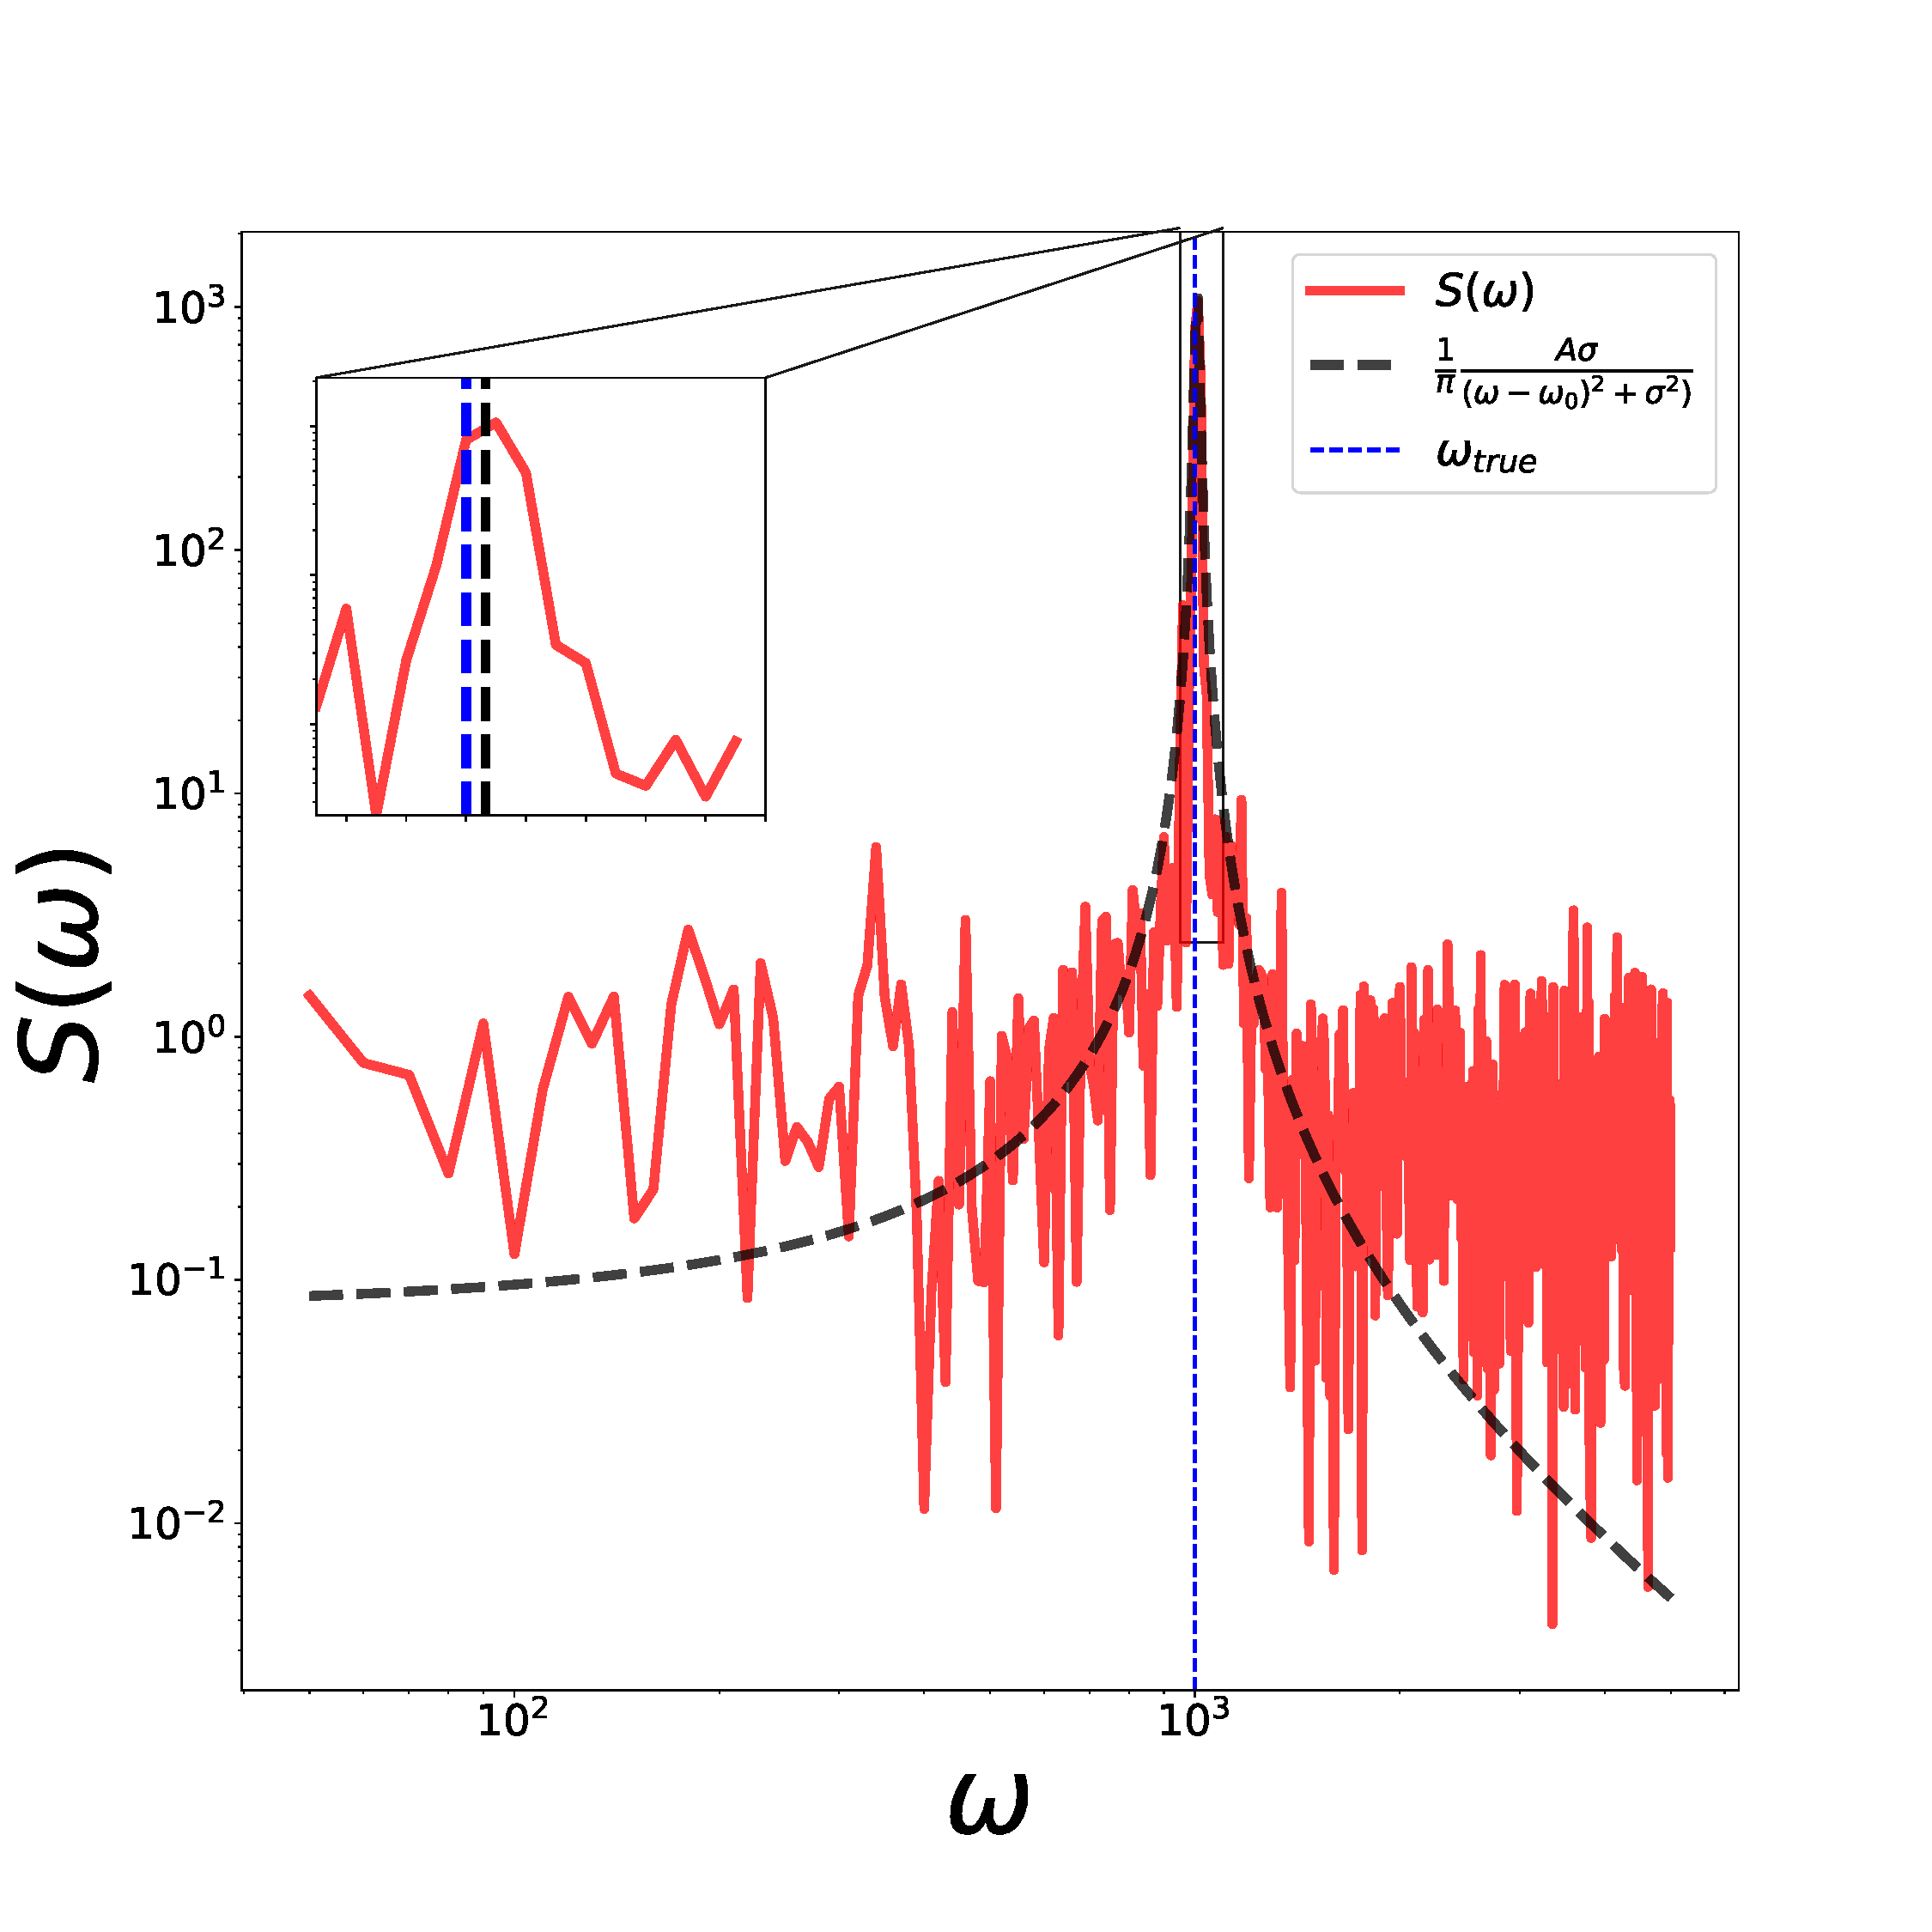
\includegraphics[width=.75\textwidth]{Figures/CMON/estimation/spectral_fit.pdf}
    \caption{We show the power spectra for a realization of the stochastic process, and the correponding Lorentzian fit.}
    \label{fig:lorentzian}
\end{figure}

\subsection{Evolution of the Fisher information}
As discussed in Sec.~\ref{ssec:1_stinf_estimation}, when estimating the value of a classical parameter, the variance of an estimator is lower bounded by the Fisher informaton, via the Cramér-Rao bound. Here, recall that given $P(\Yt;\theta)$ the probability of $\Yt$ given a known value of $\theta$, and thus the log-likelihood is defined as $\lambda(\Yt; \theta) = \log{P(\Yt;\theta)}$. Then, the Fisher information is given by
\equ{I_{t}(\theta) = \expect{(\partial_\theta \lambda(\Yt; \theta)^2} = \expect{-\partial^2_\theta \lambda(\Yt,\theta)}}
For the Gaussian system in Eq.~\ref{eq:cmon_LINEALSYSTEM}, we can readily find a dynamical equation for $\lambda_{t} \equiv \lambda(\Yt, \theta)$. In turn, by defining $\bm{u}_{t} = C \mathbf{r}_{t}$, we can write the evolution of $\partial_\theta \lambda_{t}$, obtained by taking the derivative w.r.t. $\theta$ in Eq.~\ref{eq:lambdaGauss}, as
\equ{d\partial_\theta \lambda_{t} =  - \bm{u}_{t}\cdot \partial_\theta \bm{u}_{t} dt + (\partial_\theta)\cdot \dyt.}
We can readily compute the second derivative as
\begin{align}
d \partial^2_\theta \lambda_{t} &=  - || \partial_\theta \bm{u}_{t}||^2dt - \bm{u}_{t}\cdot (\partial^2_\theta \bm{u}_{t}) dt  + (\partial^2_\theta \bm{u}_{t})\cdot \dyt\\
&= - || \partial_\theta \bm{u}_{t}||^2dt + (\partial^2_\theta\bm{u}_{t})\cdot\dwt,
\end{align}
where in the last line we have used the expression for the measurement outcome $\dyt$ in terms of the Wiener noise. In turn, the last expression with the Wiener noise turns useful, since we can readily see that the expected value $\mathbb{E}[(\partial^2_\theta\bm{u}_{t})\cdot\dwt]$ vanishes\footnote{
To see this, consider the solution
\begin{align*}
\mathbf{r}_{t} =& \chi(\cov)\int_0^t e^{-A(t-t')}dW_{t'} \\
\partial_\theta \mathbf{r}_{t} =&  \partial_\theta \chi(\cov) \int_0^t e^{-A(t-t')}d\mathbf{W}_{t'} + \chi(\cov) (\partial_\theta A) \int_0^t (t-t')e^{-A(t-t')}d\mathbf{W}_{t'} \\
\partial^2_\theta \mathbf{r}_{t} =&  \partial^2_\theta \chi(\cov) \int_0^t e^{-A(t-t')}d\mathbf{W}_{t'} + 2(\partial_\theta \chi(\cov)) (\partial_\theta A) \int_0^t (t-t') e^{-A(t-t')}d\mathbf{W}_{t'} \\ +& (\partial_\theta \chi(\cov)) (\partial_\theta A)^2 \int_0^t (t-t')^2 e^{-A(t-t')}d\mathbf{W}_{t'} + \chi(\cov) (\partial^2_\theta A) \int_0^t (t-t') e^{-A(t-t')}d\mathbf{W}_{t'}.
\end{align*}
As expected $\partial^2_\theta \mathbf{r}(t)$ is a non-anticipating function, as defined in Sec.~\ref{ssec:ito}, and thus it is uncorrelated with the Wiener noise $\dwt$ at time $t$, \textit{i.e.} $\mathbb{E}[dW_t dW_{t'}] = \delta(t-t')dt = 0$ since $0<t'<t$.
}. Thus, the Fisher info is obtained as
\equ{I_{t}(\theta) = -\mathbb{E}\Big[\partial^2_\theta \lambda_{t} \Big] =- \int_0^{t} \mathbb{E}\Big[ d\partial^2_\theta \lambda_{t}\Big],}
and we only need to integrate the values $\Big(\rbar_t, \partial_\theta \rbar_t\Big)$ in order to get it.

\begin{figure}[t!]
    \centering
    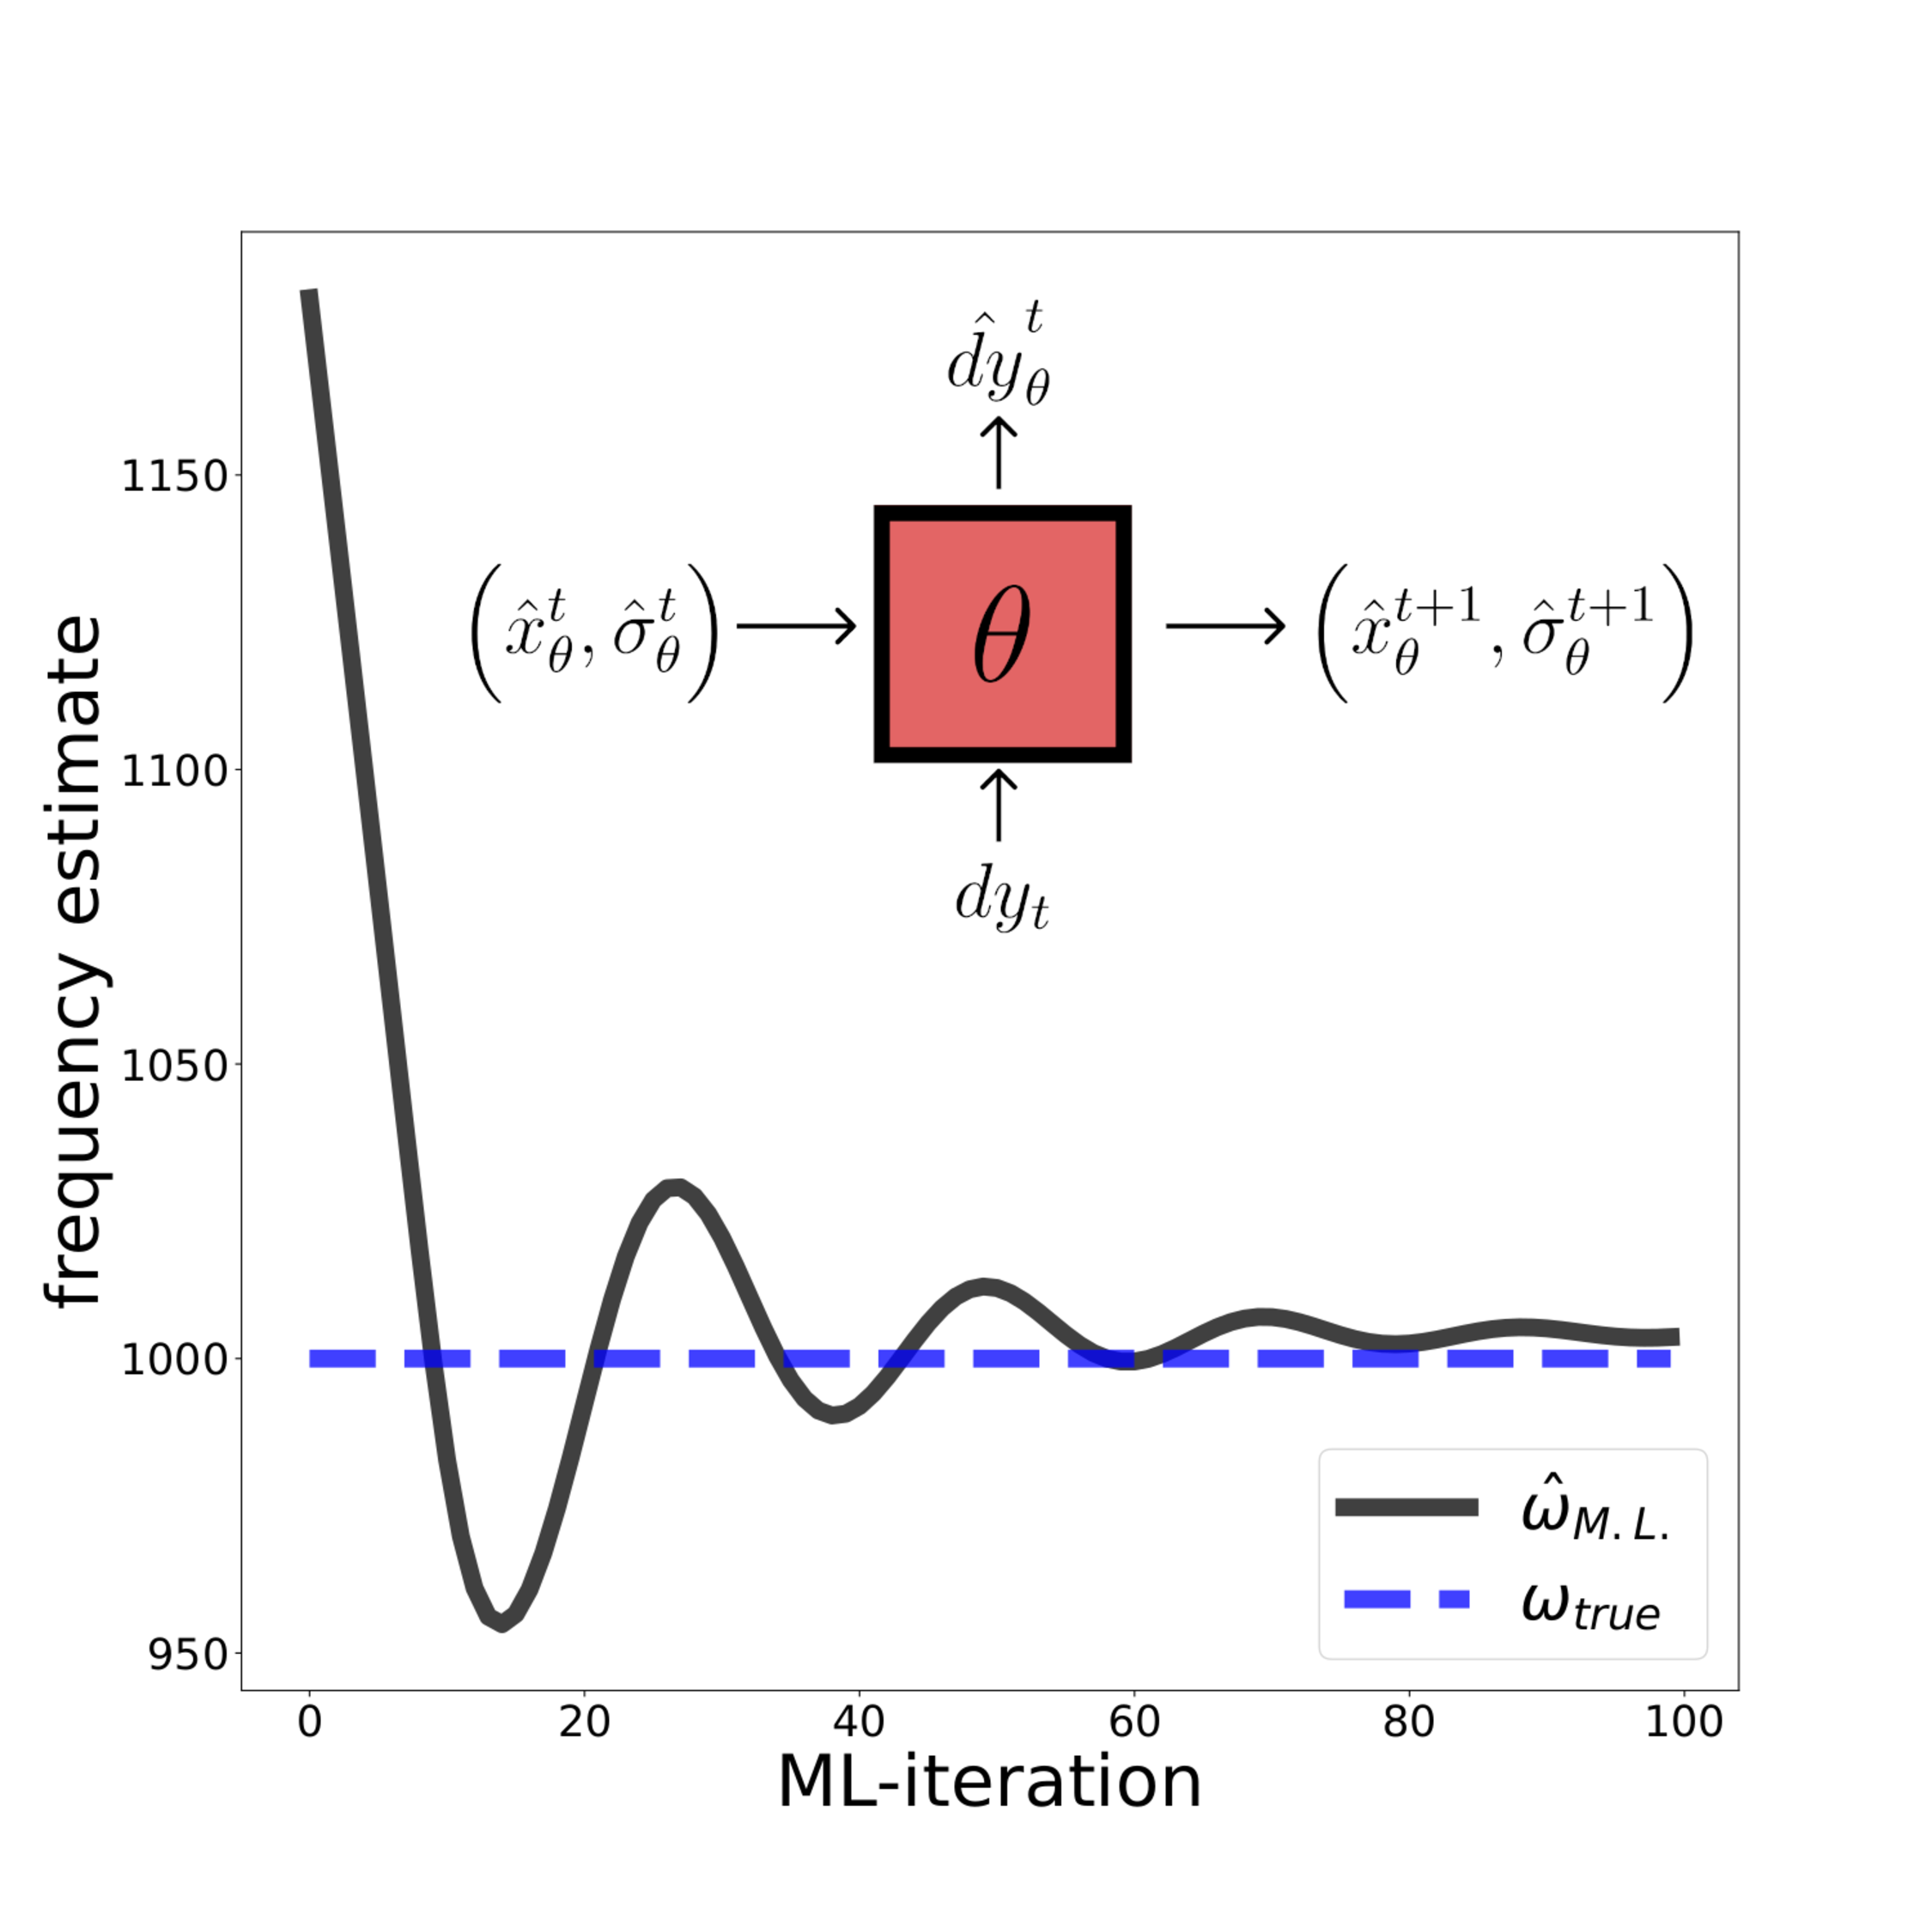
\includegraphics[width=.75\textwidth]{Figures/CMON/estimation/ml_fit_with_GRNN.pdf}
    \caption{We show the evolution for the optimization of the log-likelihood using AD, and an accompanying depiction of the recurrent cell.}
    \label{fig:rncell}
\end{figure}

\subsection{Maximum-likelihood estimation via automatic-differentiation}
While we have provided a dynamical equation for the (derivative of) the log-likelihood $\lambda(\Yt,\theta)$, here we take a step further. With the help of an automatic-differentiation (AD) library~\cite{abadi2016tensorflow}\footnote{We refer the reader to our discussion on AD in Sec.~\ref{ssec:optimizer}} we are able to implement the maximum-likelihood estimator, \textit{i.e.}
\equ{\hat{\theta} = \underset{\theta}{\text{ArgMax\;}} \lambda(\Yt, \theta).}
This optimization is done via a recurrent cell, whose structure is also shown in the Fig.~\ref{fig:rncell}. The mechanism of the cell is the following. The training consists on episodes $L=1,...,N$, and at each episode the cell has an estimate $\hat{\theta}_L$. Each episode consists on as many time-steps as the time-trace signal $\Yt$ has. At each time-step, the cell is fed with the value of the measurement outcome $\dyt$, and evolves its internal state $\hat{\mathbf{r}}_{\hat{\theta}_L}$
as per Eq.~\ref{eq:cmon_LINEALSYSTEM} (using the value $\hat{\theta}_L$).
  The cell keeps a record of such estimated hidden state, which is forwarded to the next time-step. Moreover, at each time-step, the cell outputs a predicted value for the measurement signal, given by $C \hat{\mathbf{r}}_t dt$. By the end of the time-trace, the mean squared error between all predicted values and $\Yt$ is computed. Note that the latter quantity coincides with the log-likelihood of observing $\Yt$ under $\hat{\theta}_L$. Finally, the AD mechanism is used to optimize such likelihood over $\hat{\theta}$, which is done by re-tracing the (derivative of) the likelihood and using a gradient-based method.
  Figure~\ref{fig:rncell} we also show how the estimate of the frequency improves with the number of optimization iterations.

Similarly to the Lorentzian fit, we can see in Fig.~\ref{fig:rncell} that the AD mechanism does also commits a certain error, which we expect it to be (on average) higher than the (inverse of) $I(\theta)$ --- that is, if assuming $\Yt$ was an \textit{i.i.d.} sequence---. To this end, in Fig.~\ref{fig:comparison_estimation} we compare the estimated variances of the Lorentizan fit, and the AD method, with the inverse of the Fisher information, for the frequency estimation case. This is done by carrying out the procedures outlined above for $10^{3}$ quantum trajectories. As can be seen, there seems to be a slight advantage in favour of the maximum-likelihood method.

\begin{figure}[t!]
    \centering
    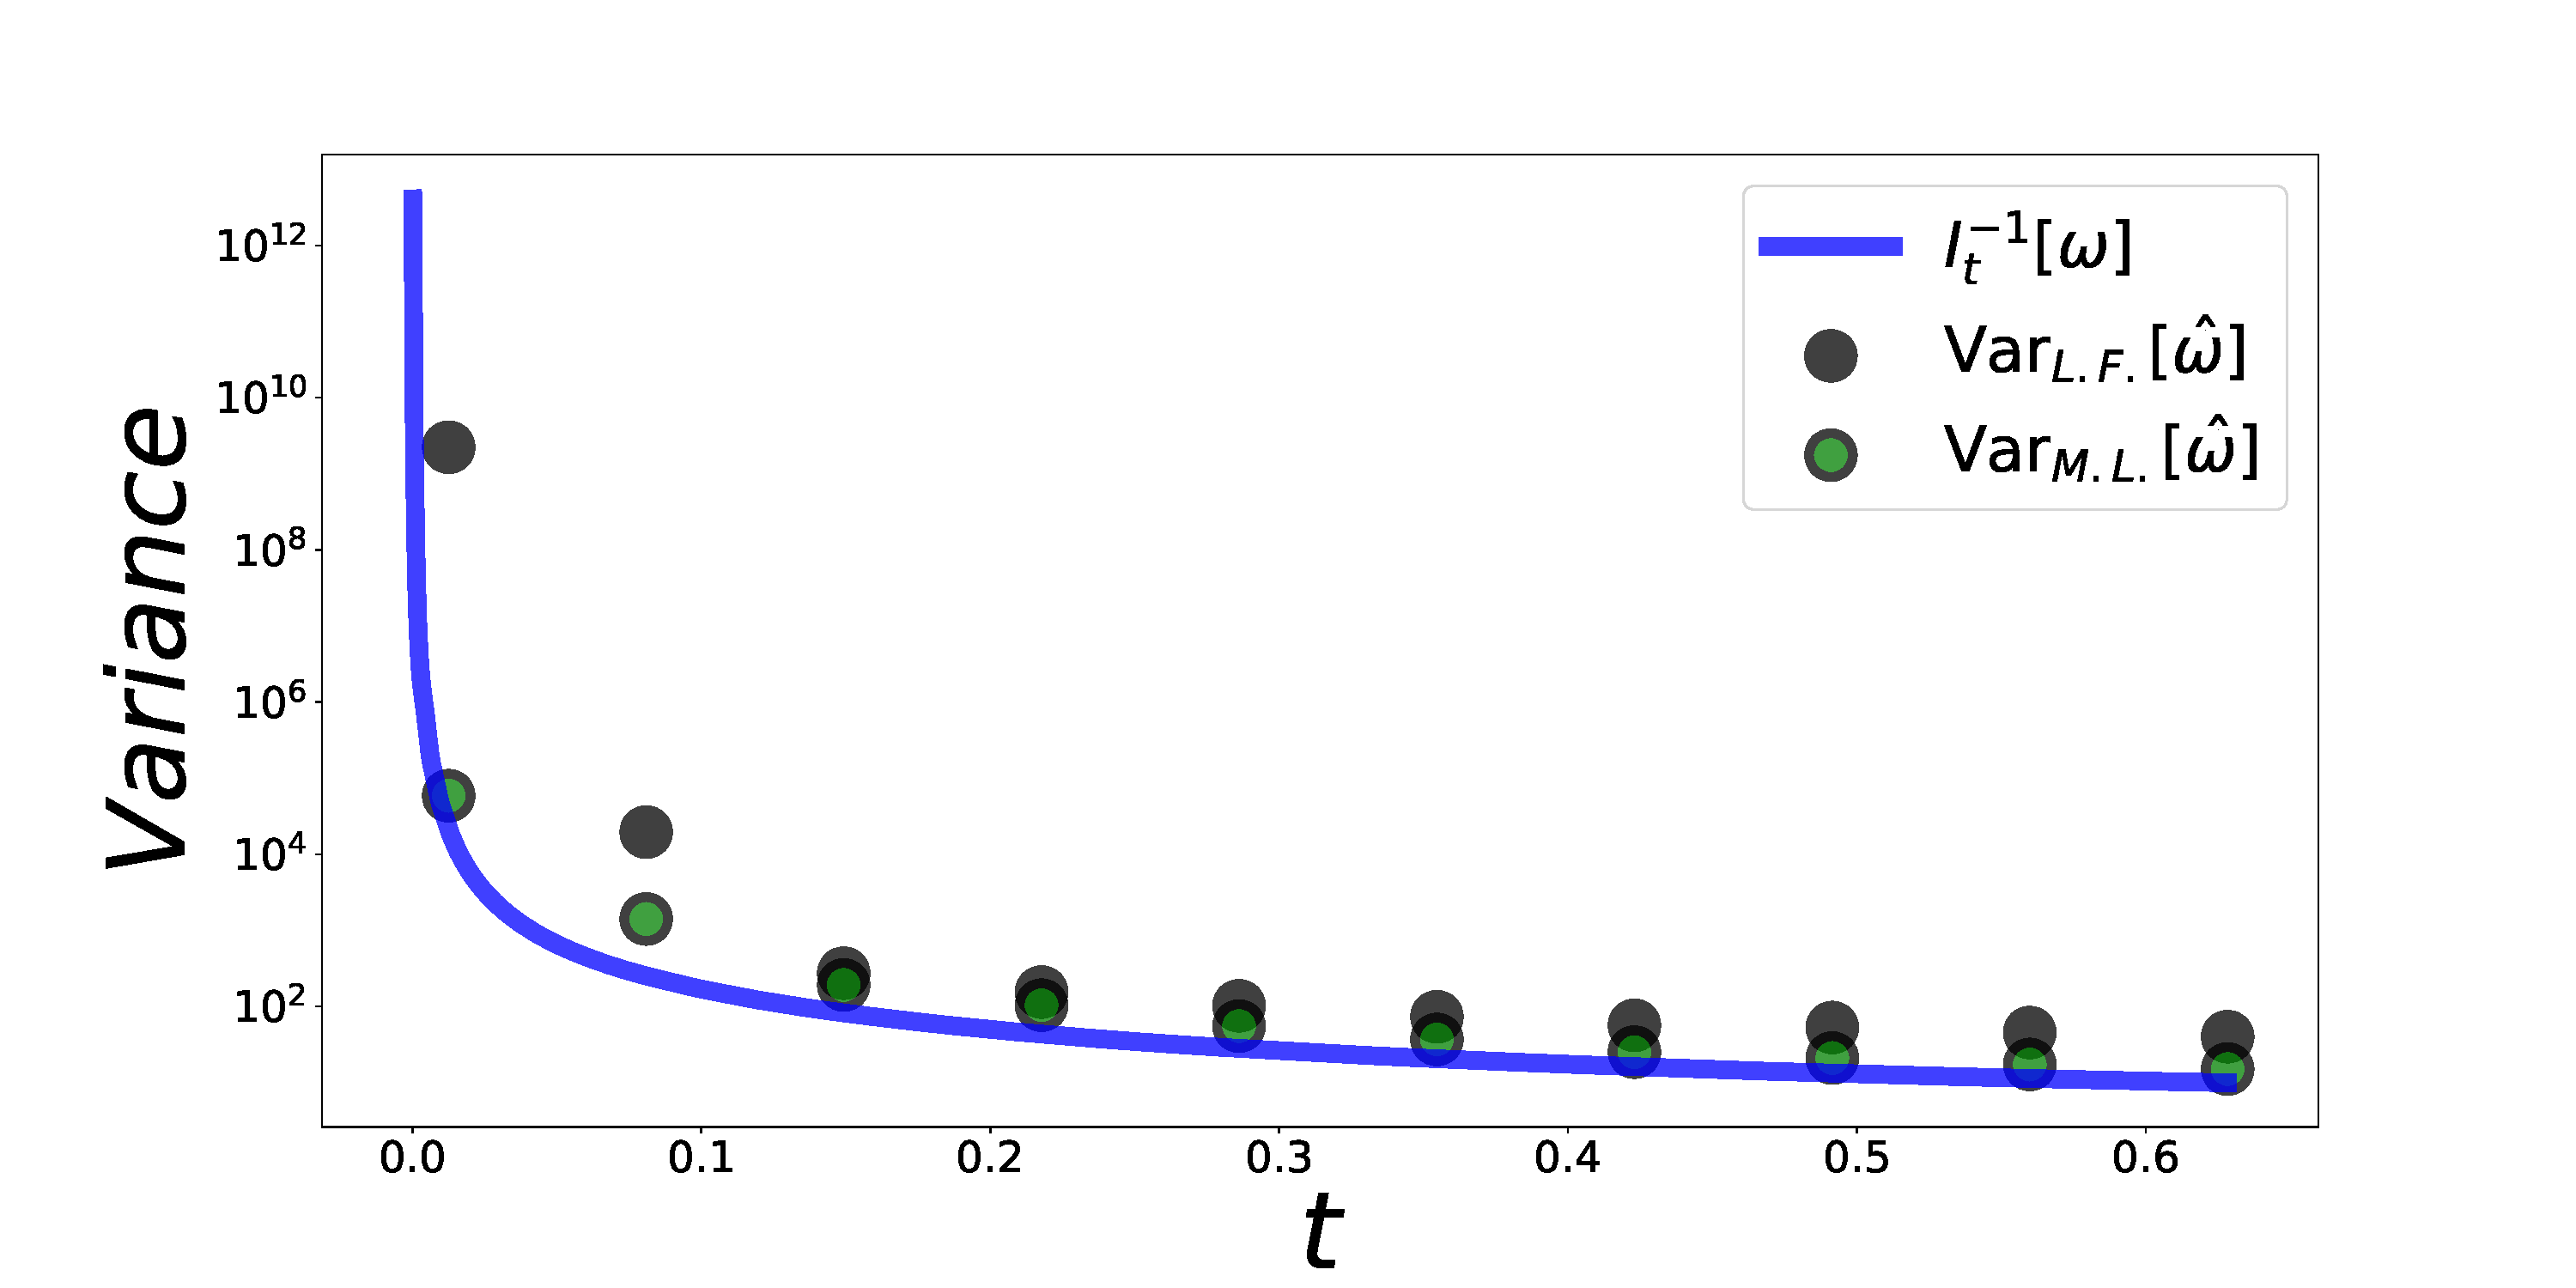
\includegraphics[width=1.\textwidth]{Figures/CMON/estimation/variance_comparison_hori.pdf}
    \caption{We compare the mean square error of the two methods discussed in the main body with the Cramér-Rao bound.}
    \label{fig:comparison_estimation}
\end{figure}

\subsection{Learning a linear force}
We have previously introduced a recurrent cell that, aided with the automatic-differentiation machinery, is able to perform maximum-likelihood estimation. Moreover, we provided an example of frequency estimation, and this constitutes an alternative to the Lorentzian fit that is traditionally used in experimental labs.

However, our approach is not aimed to replace the Lorentzian fit, but rather to complement it in cases where such fit cannot help with estimating a certain parameter. This is the case of an external drive $f^t_\theta \equiv f(t;\theta)$, which appears in the dynamics of the first moment $\rbar_t$ as an additive term~\cite{wisemanbook}. Thus, we consider the following evolution:
\equ{d\mathbf{r}_t = (A - \chi(\cov))\rbar_t + \chi(\cov) \dyt + f^t_\theta dt,}
Here, the value of the external signal might be time-dependent and depend on parameter(s) $\theta$.
Note that we have chosen the covariance matrix to take its stationary value (which does not depend on the force).

In our numerics, we consider two simple scenarios, \textit{(i)} a constant force and \textit{(ii)} an exponentially decaying force shown in Fig.~\ref{fig:forces_estimation_cmon}. In the first case, we show how the expected measurement signal value $\expect{\hat{\dyt}_{\hat{\theta}_{L}}}$ differs from the beginning of the training to the end of it. Note however that even for the untrained model, a \textit{trend} appears to be correctly reproduced. This is due to the innovation term appearing in the evolution of the hidden state, for which the \textit{true} value of $\dyt$ is injected at each time. Such fact is also illustrated in the right panel of the figure, for the exponentially-decaying case. In such example, large values of time will lead to no external signal (and thus the model will reproduce the correct dynamics), although for small values the same effect is observed. Behind such \textit{trend-reproducing} effect is the magic of Kalman filtering, which updates the probability distribution for the hidden state by means of the avaialble observations, which are generated under the underlying truth.

\begin{figure}[t!]
    \centering
    \begin{subfigure}[b]{0.49\textwidth}
        \centering
        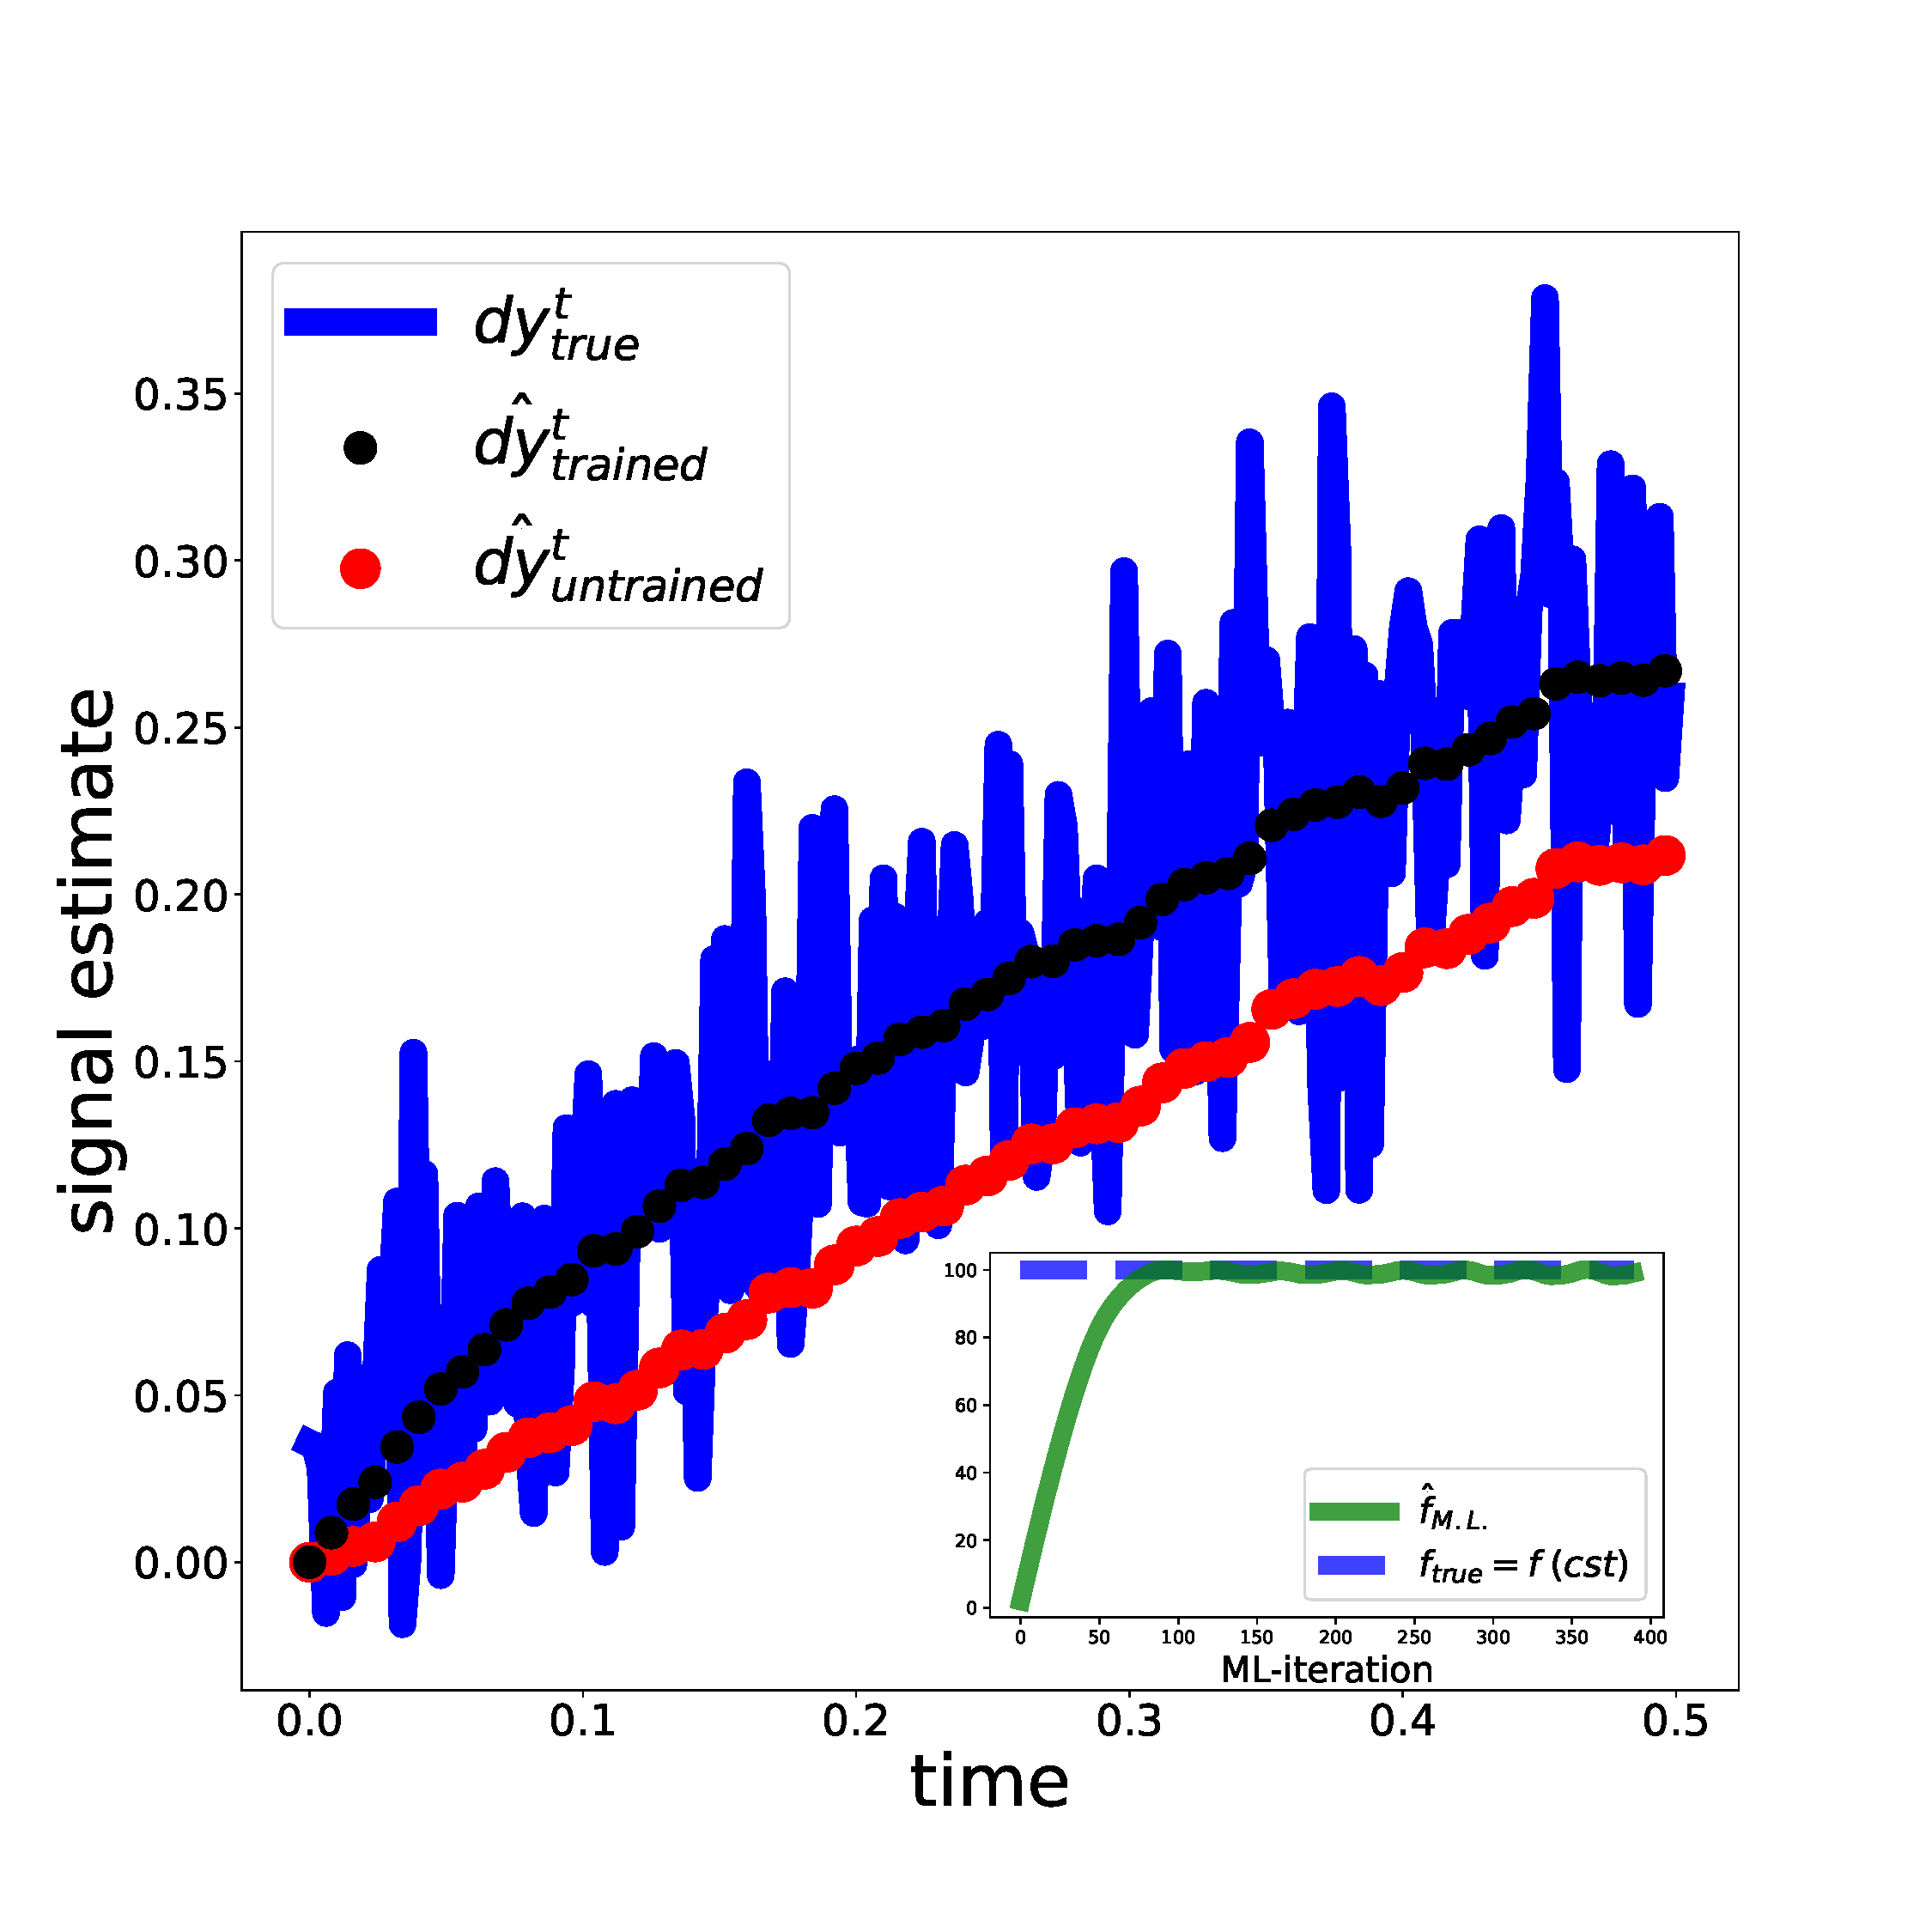
\includegraphics[width=1.\textwidth]{Figures/CMON/estimation/external_learn_signals.pdf}
        \caption{}
        \label{fig:forces1}
    \end{subfigure}
    \begin{subfigure}[b]{0.49\textwidth}
        \centering
        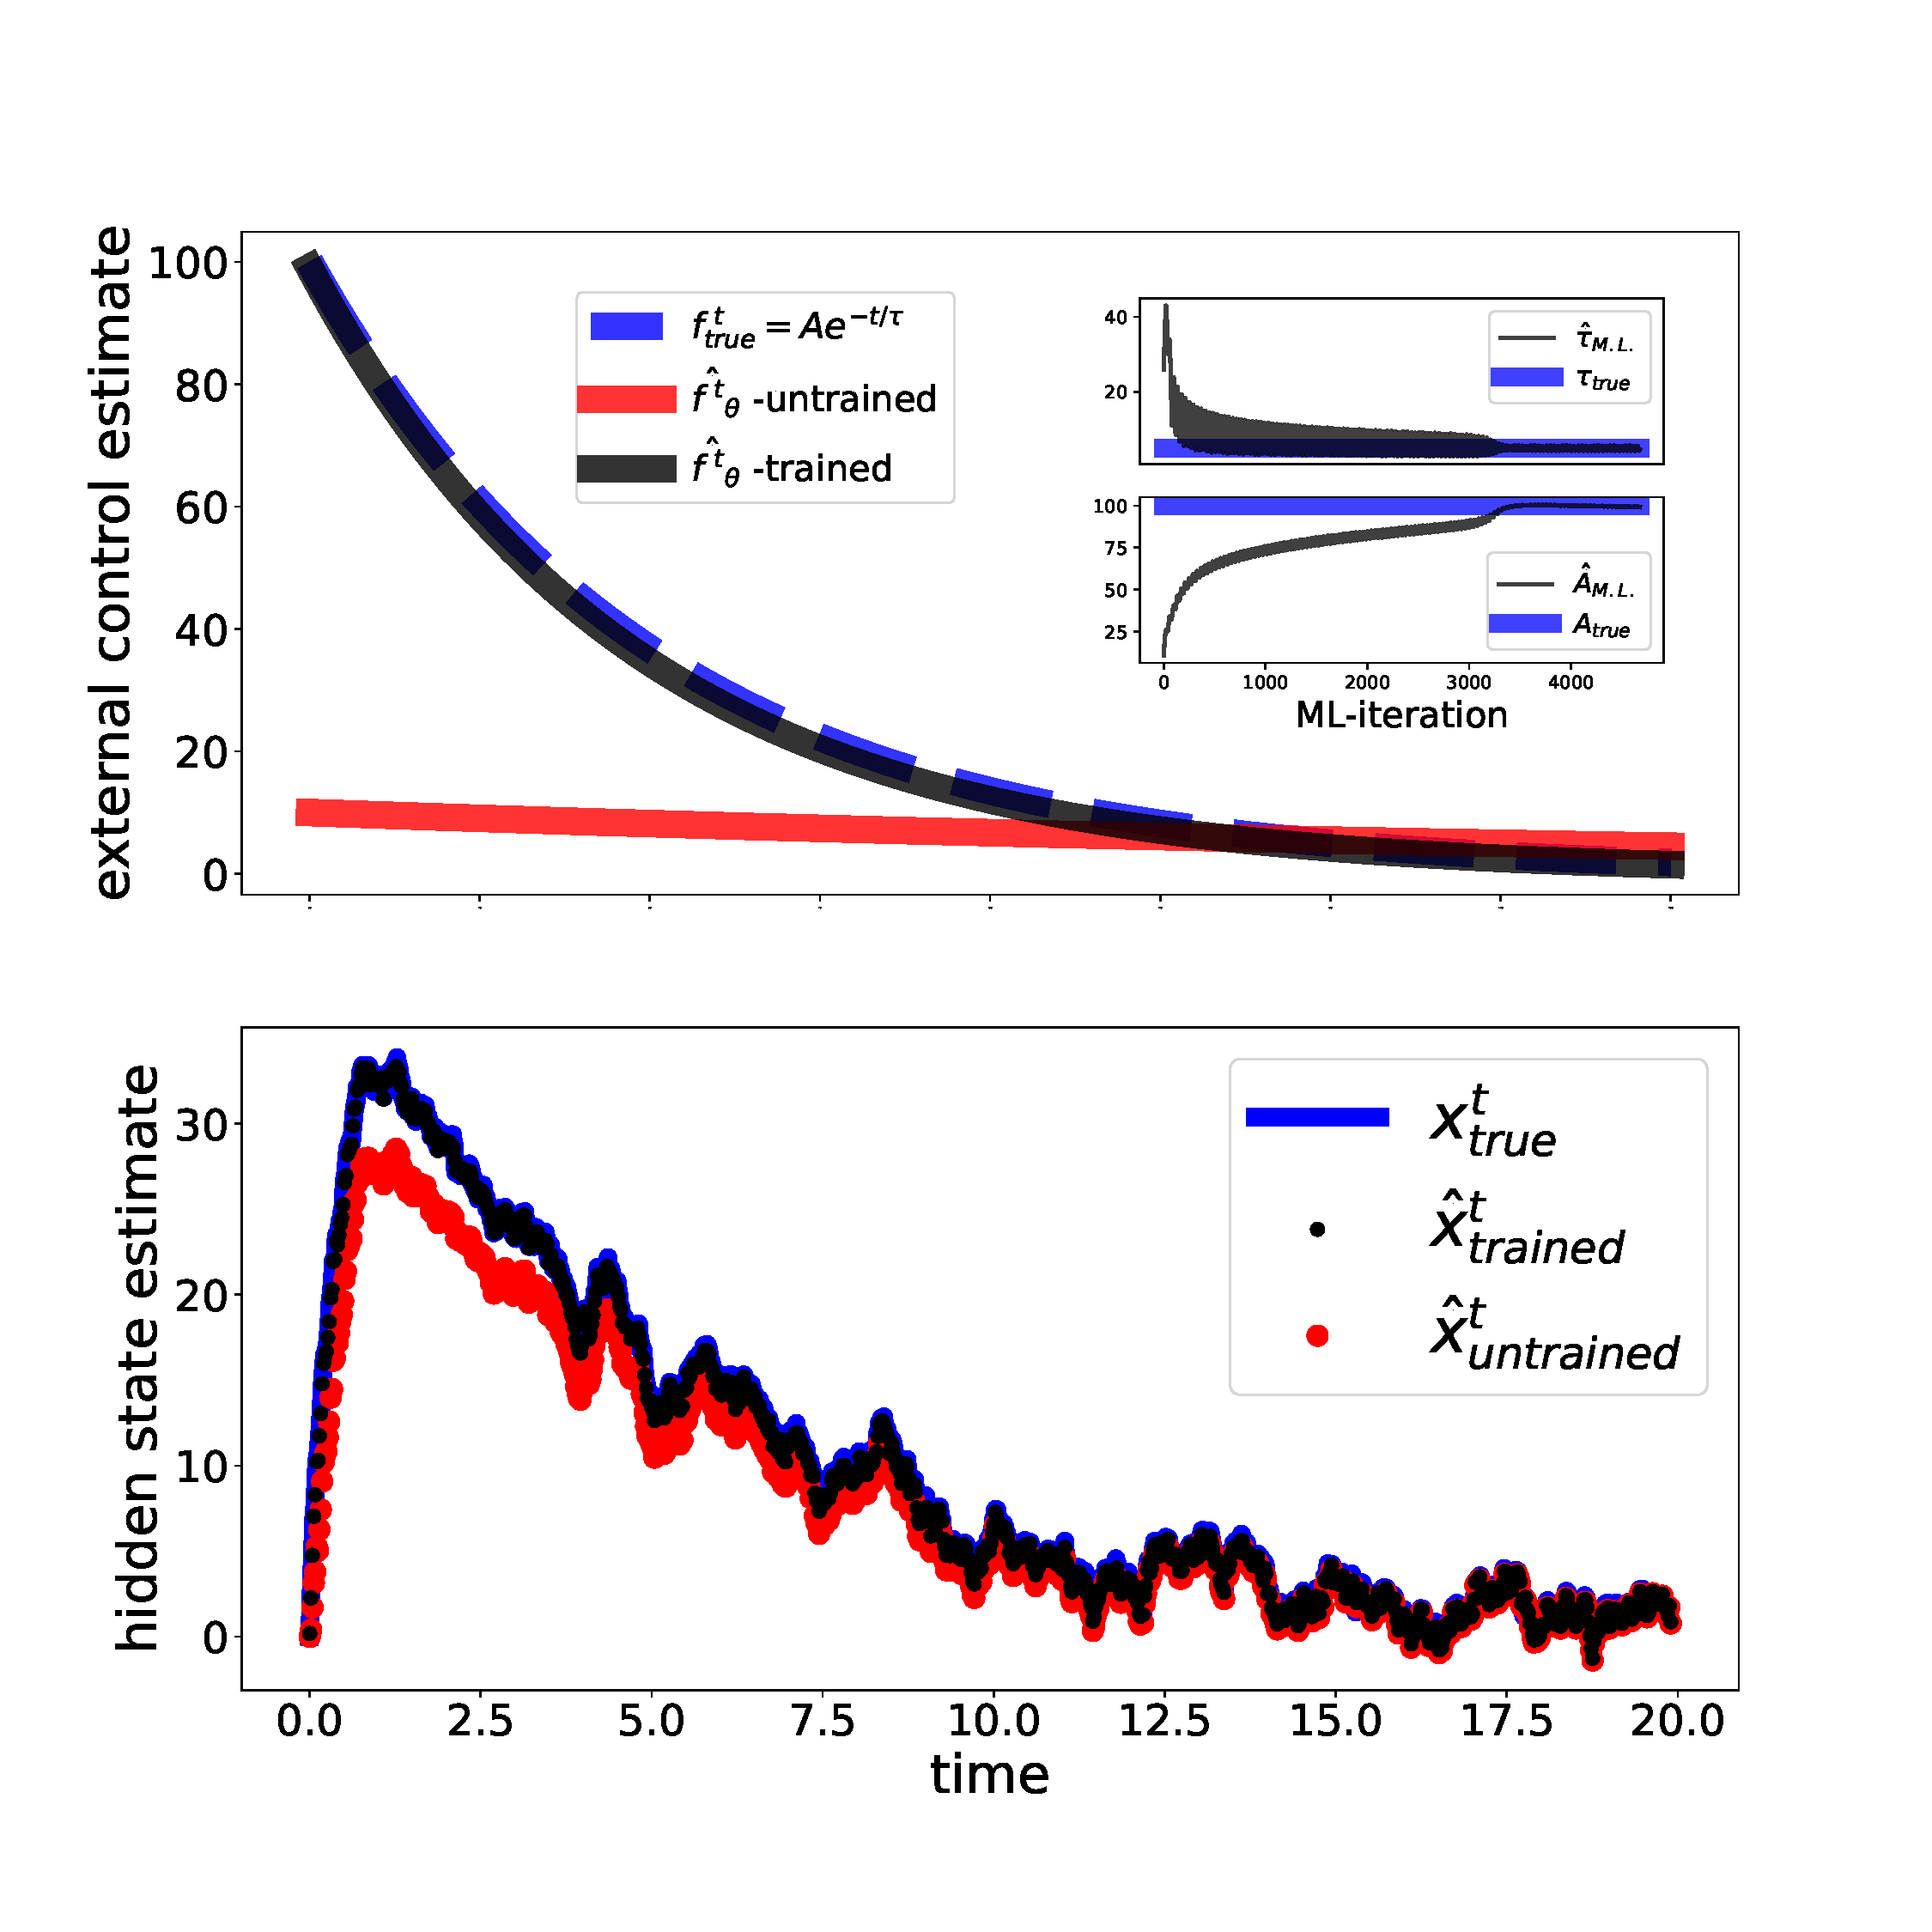
\includegraphics[width=1.\textwidth]{Figures/CMON/estimation/external_learn_track_example2.pdf}
        \caption{}
        \label{fig:forces2}
    \end{subfigure}
    \caption{We show the results of external force estimation. While the left panel consists on estimating a constant force, the right panel shows that the method learns both the amplitude and decay rate of an exponentially decaying external signal.}
    \label{fig:forces_estimation_cmon}
\end{figure}

While the examples considered in this Section are arguably simple, this method is aimed to be extended to more complex systems. In particular, we are interested in discovering dynamical equations of motion for the external signals, in the same spirit as in Ref.~\cite{sindy}, though further investigation needs to be carried out, \textit{i.e.} by the time of writing this thesis, the current is an ongoing project.

\section{Discussion $\&$ future perspectives}
In this Chapter we have analyzed statistical inference problems for continusouly monitored quantum systems.

Our main contribution is that of introducing sequential hypothesis testing strategies in such quantum regime, and elucidated an advantage in terms of a determinstic, \textit{i.e.} fixed-measurement time, strategies. On the one hand, we provided strong analytical insight on the problem, by focusing on the damping discrimination scenario. On the other, we have shown that the sequential approach can be used in different contexts, such as frequency discrimination problems.

Moreover, we have studied parameter estimation problems, and analyzed the performance of maximum-likelihood strategies, which are carried out by automatic differentiation modules. Such strategy is compared with a Lorentzian fit done on the power spectra and the mean squared errors of both strategies are compared with the Fisher information. The latter quantity is obtained by numerical integration. Furthermore, we have investigated how this approach can be used to infer parameters of external signals, and tested this on some simple examples.

Finally, it would be very interesting to derive ultimate quantum bounds for the mean stopping times under general (continuous) measurement schemes, analogous to the bound found in \cite{Vargas2021quantum, Li2022seq}. A natural way to study this problem would be to fix the coupling with the readout system (leaked light form the cavity) and optimize over the measurements done on this ancillary system.


\subsection{Code}
We refer the interested reader to Ref.~\cite{cdisc} for the hypothesis testing results (see branches \textit{damping-disc} and \textit{freq-disc}), and for the estimation results (see branch \textit{estimation} of the same reference).
